\documentclass[11pt, a4paper]{article}

% --- Encodage et langue ---
% Compatible pdflatex / xelatex / lualatex.
% Sous xelatex/lualatex, on charge fontspec (Unicode natif) ; sous pdflatex,
% on garde inputenc/fontenc + lmodern.
\usepackage{iftex}
\ifPDFTeX
  \usepackage[utf8]{inputenc}
  \usepackage[T1]{fontenc}
  \usepackage{lmodern}
  % Caractères Unicode rencontrés dans le mémoire mais non gérés par défaut.
  \DeclareUnicodeCharacter{2248}{\ensuremath{\approx}}
  \DeclareUnicodeCharacter{2265}{\ensuremath{\geq}}
  \DeclareUnicodeCharacter{2264}{\ensuremath{\leq}}
  \DeclareUnicodeCharacter{2260}{\ensuremath{\neq}}
  \DeclareUnicodeCharacter{2212}{\ensuremath{-}}
  \DeclareUnicodeCharacter{2192}{\ensuremath{\rightarrow}}
  \DeclareUnicodeCharacter{2190}{\ensuremath{\leftarrow}}
  \DeclareUnicodeCharacter{2191}{\ensuremath{\uparrow}}
  \DeclareUnicodeCharacter{2193}{\ensuremath{\downarrow}}
  \DeclareUnicodeCharacter{2194}{\ensuremath{\leftrightarrow}}
  \DeclareUnicodeCharacter{21D2}{\ensuremath{\Rightarrow}}
  \DeclareUnicodeCharacter{2026}{\ldots}
  \DeclareUnicodeCharacter{2075}{\ensuremath{^{5}}}
  \DeclareUnicodeCharacter{2076}{\ensuremath{^{6}}}
  \DeclareUnicodeCharacter{25BA}{\ensuremath{\blacktriangleright}}
  \DeclareUnicodeCharacter{25C4}{\ensuremath{\blacktriangleleft}}
  \DeclareUnicodeCharacter{2500}{-}
  \DeclareUnicodeCharacter{2502}{|}
  \DeclareUnicodeCharacter{250C}{+}
  \DeclareUnicodeCharacter{2510}{+}
  \DeclareUnicodeCharacter{2514}{+}
  \DeclareUnicodeCharacter{2518}{+}
  \DeclareUnicodeCharacter{2082}{\textsubscript{2}}
\else
  \usepackage{fontspec}
  \defaultfontfeatures{Ligatures=TeX}
  % « Arial » (équivalent libre métrique-compatible fourni par texlive-fonts-recommended).
  \setmainfont{TeX Gyre Heros}
  \setsansfont{TeX Gyre Heros}
  \setmonofont{TeX Gyre Cursor}
\fi
\usepackage[french]{babel}

% --- Caractères Unicode manquants (valable pdflatex ET xelatex/lualatex) ---
\usepackage{newunicodechar}
\newunicodechar{≈}{\ensuremath{\approx}}
\newunicodechar{≥}{\ensuremath{\geq}}
\newunicodechar{≤}{\ensuremath{\leq}}
\newunicodechar{≠}{\ensuremath{\neq}}
\newunicodechar{⇒}{\ensuremath{\Rightarrow}}
\newunicodechar{→}{\ensuremath{\rightarrow}}
\newunicodechar{←}{\ensuremath{\leftarrow}}
\newunicodechar{↑}{\ensuremath{\uparrow}}
\newunicodechar{↓}{\ensuremath{\downarrow}}
\newunicodechar{↔}{\ensuremath{\leftrightarrow}}
\newunicodechar{−}{\ensuremath{-}}
\newunicodechar{…}{\ldots}
\newunicodechar{⁵}{\ensuremath{^{5}}}
\newunicodechar{⁶}{\ensuremath{^{6}}}
\newunicodechar{►}{\ensuremath{\blacktriangleright}}
\newunicodechar{◄}{\ensuremath{\blacktriangleleft}}
\newunicodechar{─}{\texttt{-}}
\newunicodechar{│}{\texttt{|}}
\newunicodechar{┌}{\texttt{+}}
\newunicodechar{┐}{\texttt{+}}
\newunicodechar{└}{\texttt{+}}
\newunicodechar{┘}{\texttt{+}}
\newunicodechar{₂}{\textsubscript{2}}

% --- Mise en page ---
\usepackage[margin=2.5cm]{geometry}
\usepackage{setspace}
\setstretch{1.15}
\setcounter{secnumdepth}{-1}

% --- Titres : forcer \paragraph et \subparagraph à passer à la ligne ---
% Par défaut LaTeX rend \paragraph (= #### Markdown) en titre « run-in »,
% collé au début du paragraphe qui suit. On les redéfinit en blocs.
\usepackage{titlesec}
\titleformat{\paragraph}[block]
  {\normalfont\normalsize\bfseries}{\theparagraph}{1em}{}
\titlespacing*{\paragraph}
  {0pt}{2.25ex plus 1ex minus .2ex}{1ex plus .2ex}
\titleformat{\subparagraph}[block]
  {\normalfont\normalsize\bfseries\itshape}{\thesubparagraph}{1em}{}
\titlespacing*{\subparagraph}
  {0pt}{2ex plus 1ex minus .2ex}{0.8ex plus .2ex}

% --- Anti-débordement (inline code, longs identifiants, URLs) ---
% Pandoc convertit `code` en \texttt{...}. Par défaut, la fonte monospace
% interdit toute coupure : les identifiants type « recursive-1024-128 »
% débordent en marge.
% Stratégie :
%   (a) marge d'élasticité d'urgence + \sloppy,
%   (b) coupure aux tirets « - » réactivée dans la fonte monospace,
%   (c) le paquet « underscore » rend « \_ » sécable en mode texte,
%       ce qui permet le retour à la ligne après un « _ » dans les
%       identifiants type « entité_émettrice », sans couper le mot
%       au milieu d'une syllabe.
\setlength{\emergencystretch}{4em}
\usepackage[strings]{underscore}

\makeatletter
% Active la coupure aux tirets « - » dans la fonte monospace
\renewcommand\ttfamily{%
  \not@math@alphabet\ttfamily\mathtt
  \fontfamily\ttdefault\selectfont
  \hyphenchar\font=`\-\relax}
\makeatother

% --- Maths ---
\usepackage{amsmath, amssymb, amsfonts}

% --- Tableaux et figures ---
\usepackage{array}
\usepackage{calc}
\usepackage{booktabs}
\usepackage{longtable}
\usepackage{graphicx}
\makeatletter
\def\maxwidth{\ifdim\Gin@nat@width>\linewidth\linewidth\else\Gin@nat@width\fi}
\def\maxheight{\ifdim\Gin@nat@height>\textheight\textheight\else\Gin@nat@height\fi}
\makeatother
\setkeys{Gin}{width=\maxwidth,height=\maxheight,keepaspectratio}
\usepackage{float}

% --- Liens ---
\usepackage[colorlinks=true, linkcolor=blue!60!black, citecolor=blue!60!black, urlcolor=blue!60!black]{hyperref}

% --- Support pour les tables sans légende Pandoc 3.8+ ---
\newcounter{none}
\providecommand{\theHnone}{\thenone}

% --- Code ---
% Build uses pandoc --no-highlight, so we provide minimal Shaded / Highlighting
% environments ourselves (pandoc still wraps code blocks in them).
\usepackage{listings}
\usepackage{xcolor}
\usepackage{fancyvrb}
\usepackage{framed}
\definecolor{shadecolor}{RGB}{248,248,248}
\newenvironment{Shaded}{\begin{snugshade}}{\end{snugshade}}
\DefineVerbatimEnvironment{Highlighting}{Verbatim}{commandchars=\\\{\}}

% --- Notes de bas de page (footnotes Pandoc) ---
\usepackage{footnote}

% --- En-têtes / pieds de page ---
\usepackage{fancyhdr}
\pagestyle{fancy}
\setlength{\headheight}{28pt}
\fancyhf{}
\fancyhead[L]{\nouppercase{\leftmark}}
\fancyhead[R]{\thepage}
\renewcommand{\headrulewidth}{0.4pt}
% Classe « article » : \leftmark est alimenté par \sectionmark.
\renewcommand{\sectionmark}[1]{\markboth{#1}{}}

% --- Titre ---
\title{Jumeaux Numériques et Intelligence Artificielle Topologique :
Vers une prédiction instantanée de la résilience et des émissions
urbaines}
\author{Thomas Clerc}
\date{2026}

% --- Pandoc tight list ---
% Pandoc insère \tightlist au début des listes serrées (items sans ligne
% vide entre eux). La définition par défaut écrase tout espace vertical,
% ce qui rend les puces illisibles. On la neutralise pour conserver les
% espacements standards de \itemize.
\providecommand{\tightlist}{}

% --- Pandoc syntax highlighting macros ---

% --- CSL refs (Pandoc --citeproc) ---

\begin{document}

% --- Page de titre ---
\begin{titlepage}
\centering
\vspace*{2cm}
{\Huge\bfseries Jumeaux Numériques et Intelligence Artificielle
Topologique : Vers une prédiction instantanée de la résilience et des
émissions urbaines\par}
\vspace{1.5cm}
{\Large Mémoire\par}
\vspace{1cm}
{\large Thomas Clerc\par}
\vspace{0.5cm}
{\large 2026\par}
\vfill
\end{titlepage}

% --- Table des matières ---
\tableofcontents
\newpage

% --- Corps ---
\section{RÉSUMÉ \& MOTS-CLÉS}\label{ruxe9sumuxe9-mots-cluxe9s}

\subsubsection{Résumé}\label{ruxe9sumuxe9}

Ce mémoire de fin d'études présente un cadre méthodologique de rupture
pour l'évaluation et la prédiction en temps réel des émissions de
\(CO_2\) du trafic routier à l'échelle de réseaux urbains globaux. La
planification urbaine durable se heurte historiquement à un verrou
computationnel majeur : les micro-simulateurs physiques multi-agents
(comme SUMO), bien que précis pour modéliser le comportement individuel
des véhicules, s'avèrent extrêmement coûteux en temps de calcul CPU et
en mémoire RAM, interdisant toute exploration dynamique de scénarios à
grande échelle ou d'aide à la décision en temps réel.

Pour briser ce goulot d'étranglement, ce travail de recherche propose
une méthodologie originale basée sur l'\textbf{Intelligence Artificielle
Topologique Spectrale}. En traduisant la voirie de n'importe quelle
ville sous forme de matrice d'adjacence orientée et pondérée par
l'impédance physique, nous extrayons des signatures spectrales avancées
issues de la théorie des graphes non-normaux (rayon spectral, constante
de Kreiss, perturbations de Kato, normes de Hardy \(H_2/H_\infty\)). Ces
descripteurs topologiques décrivent mathématiquement la résilience et la
vulnérabilité intrinsèques d'un réseau face à la congestion. En
associant ces signatures mathématiques à un modèle d'apprentissage
supervisé XGBoost entraîné sur un corpus multi-villes diversifié, notre
modèle estime instantanément (en moins de 0,2 seconde) les émissions
globales de \(CO_2\) pour des volumes et des compositions de trafic
arbitraires. Les résultats démontrent une précision de prédiction
supérieure à 95 \% (RMSE de 13,4 tonnes de \(CO_2\)), validant la
généralisation du modèle sur des structures urbaines inédites.

En outre, la pertinence opérationnelle de ce cadre prédictif est
démontrée à travers une étude de cas microscopique locale calibrée par
vision par ordinateur (YOLOv8) sur le hub de recharge de Vinhomes Ocean
Park (Hanoï), illustrant comment l'IA s'interface avec les
micro-simulations pour guider les politiques de mitigation et la
transition vers l'électromobilité.

\subsubsection{Mots-clés}\label{mots-cluxe9s}

Analyse Spectrale, Graphes Non-Normaux, Constante de Kreiss, Théorie des
Perturbations de Kato, XGBoost, Métamodèle Prédictif, Micro-simulation,
SUMO, Mobilité Durable, Vinhomes Ocean Park, Hanoï.

\newpage

\section{REMERCIEMENTS}\label{remerciements}

Je tiens à exprimer ma profonde gratitude à l'ensemble des personnes qui
ont contribué au succès de ce travail de recherche et à l'aboutissement
de mon cursus de fin d'études.

Tout d'abord, je remercie chaleureusement mes tuteurs académiques,
\textbf{M. Pierre Uzarralde} et \textbf{M. Alain Faye}, pour leur suivi
rigoureux, leurs conseils méthodologiques et leur exigence scientifique
tout au long de la rédaction de ce mémoire.

Je tiens également à remercier l'École Hexagone, qui m'a permis de
réaliser ce projet et d'effectuer ce séjour d'études et de recherche au
Vietnam.

Mes remerciements s'adressent également aux équipes de recherche en
mobilité intelligente de l'Université \textbf{VinUniversity} à Hanoï
(Vietnam), qui m'ont accueilli lors de mon séjour de recherche et m'ont
fourni les moyens matériels et de collecte de données nécessaires à
cette étude.

Enfin, je remercie chaleureusement ma famille et mes proches pour leur
soutien indéfectible durant cette année académique.

\newpage

\section{GLOSSAIRE DES TERMES TECHNIQUES ET
MATHÉMATIQUES}\label{glossaire-des-termes-techniques-et-mathuxe9matiques}

\begin{itemize}
\tightlist
\item
  \textbf{Jumeau Numérique (Digital Twin) :} Réplication virtuelle
  dynamique d'un système physique réel (ici, la voirie et la cinématique
  des flux de trafic d'une ville) permettant d'effectuer des tests, de
  simuler des scénarios d'aménagements et de guider la prise de
  décision.
\item
  \textbf{Micro-simulation microscopique :} Modélisation individuelle du
  comportement de chaque agent mobile (vitesse, position, distance de
  sécurité) à chaque pas de temps discret, par opposition aux modèles
  macroscopiques basés sur des équations d'écoulement de fluides moyens.
\item
  \textbf{Mésoscopique :} Modèle de simulation hybride intermédiaire
  dans lequel les flux de trafic ne sont pas calculés véhicule par
  véhicule, mais modélisés sous forme de files d'attente de paquets
  d'agents se déplaçant le long de segments de voies, réduisant
  significativement la charge computationnelle.
\item
  \textbf{TraCI (Traffic Control Interface) :} API native du framework
  SUMO permettant le contrôle et la modification temps réel des états de
  simulation (feux, départs, itinéraires) via un script externe
  (généralement écrit en Python).
\item
  \textbf{Matrice d'Adjacence :} Représentation matricielle carrée de
  taille \(n \times n\) (où \(n\) est le nombre de nœuds) décrivant les
  connexions d'un graphe. Dans le cadre de l'ingénierie routière, elle
  est asymétrique pour modéliser les sens uniques et pondérée
  physiquement par le rapport temps de parcours/capacité des voies.
\item
  \textbf{Opérateur Laplacien :} Matrice définie par \(L = D - A\) (ou
  ses variantes normalisées) décrivant les flux de diffusion sur le
  graphe de la voirie. Ses valeurs propres caractérisent la connectivité
  structurelle du réseau.
\item
  \textbf{Rayon Spectral (\(\rho\)) :} Module de la valeur propre
  dominante d'une matrice. En topologie urbaine, il caractérise la
  capacité globale de transit et la hiérarchisation des corridors de
  circulation.
\item
  \textbf{Non-normalité :} Propriété d'une matrice qui ne commute pas
  avec sa transposée (\(A A^T \neq A^T A\)). Caractérise les réseaux
  urbains asymétriques et indique la possibilité d'amplifications
  transitoires du trafic.
\item
  \textbf{Constante de Kreiss (\(K\)) :} Métrique caractérisant
  l'amplitude maximale de l'amplification transitoire des perturbations
  avant le retour à l'équilibre asymptotique, traduisant la
  vulnérabilité d'un réseau aux embouteillages en cascade.
\item
  \textbf{Normes de Hardy (\(H_2 / H_\infty\)) :} Normes d'espaces
  fonctionnels décrivant la réponse d'un système dynamique aux
  perturbations. \(H_\infty\) caractérise le gain maximal dans le pire
  scénario de charge, tandis que \(H_2\) caractérise la persistance
  temporelle de l'énergie de perturbation stockée (mémoire de la
  congestion).
\item
  \textbf{Théorie des Perturbations de Kato :} Formalisme mathématique
  permettant de dériver analytiquement les variations du spectre d'un
  opérateur linéaire soumis à une perturbation mineure (par exemple,
  calculer l'impact de la fermeture d'un pont sur les valeurs propres de
  transit sans recalculer le système complet).
\item
  \textbf{XGBoost (eXtreme Gradient Boosting) :} Algorithme
  d'apprentissage supervisé basé sur le boosting d'arbres de décision
  régularisé, optimisant une fonction de coût complexe via un
  développement de Taylor de second ordre.
\item
  \textbf{YOLOv8 (You Only Look Once, v8) :} Modèle de réseau de
  neurones convolutif monocoup optimisé pour le traitement d'images
  temps réel, réalisant la détection, la classification et le suivi
  d'objets (véhicules).
\item
  \textbf{Dwell Time (Temps d'arrêt) :} Durée d'immobilisation physique
  d'un véhicule à une borne pour réaliser sa session de recharge
  électrique, modélisée sous forme de loi normale tronquée.
\item
  \textbf{Warm-Start (Démarrage à chaud) :} Initialisation d'une
  simulation dans un état pré-chargé (hub de recharge occupé
  stochastiquement par des véhicules fantômes) pour supprimer le biais
  transitoire du démarrage à vide.
\item
  \textbf{Spillback (Refoulement) :} Phénomène de propagation d'un
  bouchon où la file d'attente accumulée sur une voie sature et déborde
  pour paralyser les intersections situées en amont.
\item
  \textbf{SWAP (Pagination) :} Mécanisme du noyau système consistant à
  utiliser une partie de l'espace disque comme mémoire virtuelle lente
  lorsque la mémoire vive (RAM) physique est saturée.
\end{itemize}

\newpage

\section{LISTE DES ILLUSTRATIONS}\label{liste-des-illustrations}

\begin{itemize}
\tightlist
\item
  \textbf{Figure 1 :} Distribution temporelle de la flotte d'autobus
  publics à Sao Bien (\emph{Chapitre 3, Section 1}).
\item
  \textbf{Figure 2 :} Structure modale du trafic en période régulière de
  mi-journée (Regular Midday) (\emph{Chapitre 3, Section 1}).
\item
  \textbf{Figure 3 :} Structure modale du trafic en heure de pointe de
  soirée (Evening Rush Hour) (\emph{Chapitre 3, Section 1}).
\item
  \textbf{Figure 4 :} Répartition modale comparée du fluide de trafic
  (Midi Régulier vs Holiday Reversal) (\emph{Chapitre 3, Section 1}).
\item
  \textbf{Figure 5 :} Évolution de la structure modale du trafic selon
  les périodes (Midi régulier, Transition, Vacances) (\emph{Chapitre 3,
  Section 1}).
\item
  \textbf{Figure 6 :} Taux de pénétration des véhicules électriques (EV)
  au sein de la flotte de quatre roues (\emph{Chapitre 3, Section 1}).
\item
  \textbf{Figure 7 :} Évolution journalière des volumes de trafic par
  créneaux horaires à Sao Bien (Hanoï) (\emph{Chapitre 3, Section 1}).
\item
  \textbf{Figure 8 :} Profil d'intensité horaire global du trafic sur
  l'avenue Sao Bien (\emph{Chapitre 3, Section 1}).
\item
  \textbf{Figure 9 :} Analyse de corrélation et résidus (Scatter Plot)
  de la validation croisée IA vs SUMO sur les 27 scénarios des 9 villes
  tests (\emph{Chapitre 3, Section 2}).
\item
  \textbf{Figure 10 :} Capture d'écran de l'interface utilisateur
  Streamlit - Configuration du scénario de trafic (\emph{Chapitre 3,
  Section 2}).
\item
  \textbf{Figure 11 :} Visualisation SIG de la ville test (Illustration
  de la cartographie des congestions) (\emph{Chapitre 3, Section 2}).
\end{itemize}

\newpage

\section{LISTE DES TABLEAUX}\label{liste-des-tableaux}

\begin{itemize}
\tightlist
\item
  \textbf{Tableau 1 :} Caractéristiques topologiques générales des 21
  villes étudiées (nombre de nœuds, d'arêtes, densité de connexion,
  degré moyen, indice d'asymétrie, ratio de sources et de puits)
  (\emph{Chapitre 2, Section 2}).
\item
  \textbf{Tableau 2 :} Métriques spectrales de non-normalité des
  matrices d'adjacence non pondérées pour les 21 réseaux urbains
  (asymétrie, rayon spectral, valeur singulière maximale, norme \(H_2\),
  constante de Kreiss) (\emph{Chapitre 2, Section 2}).
\item
  \textbf{Tableau 3 :} Performances comparatives des modèles
  d'apprentissage machine pour la prédiction directe des émissions de
  \(CO_2\) (RMSE, MAE, \(R^2\) de XGBoost, Ridge, Random Forest et MLP)
  (\emph{Chapitre 2, Section 3}).
\item
  \textbf{Tableau 4 :} Profil d'importance des variables (\emph{Feature
  Importance}) dans le modèle final de prédiction de \(CO_2\) par
  XGBoost (\emph{Chapitre 2, Section 3}).
\item
  \textbf{Tableau 4b :} Répartition modale du trafic en période
  régulière (Midday Baseline) (\emph{Chapitre 3, Section 1}).
\item
  \textbf{Tableau 4c :} Répartition modale du trafic en heure de pointe
  régulière (Regular Evening Peak) (\emph{Chapitre 3, Section 1}).
\item
  \textbf{Tableau 4d :} Comparaison de la structure de trafic : Semaine
  Régulière vs Période de Vacances (Holiday Reversal) (\emph{Chapitre 3,
  Section 1}).
\item
  \textbf{Tableau 5 :} Taille géométrique des fichiers net.xml sur
  disque et occupation correspondante de la mémoire RAM en Python
  (filtrage DOM via sumolib) pour cinq villes types (\emph{Chapitre 3,
  Section 2}).
\item
  \textbf{Tableau 6 :} Résultats de la validation croisée
  (Generalization Cross-City) de l'IA face aux simulations physiques
  SUMO de référence pour trois configurations cibles (Nelson, Maseru et
  Pamplona) (\emph{Chapitre 3, Section 2}).
\item
  \textbf{Tableau 6b :} Matrice comparative de la validation croisée
  étendue (IA vs SUMO) sur 9 villes inédites sous 3 scénarios de charge
  (\emph{Chapitre 3, Section 2}).
\item
  \textbf{Tableau 7 :} Extrait représentatif de 17 simulations parmi les
  50 simulations complètes du framework multi-villes agnostique
  (véhicules, vitesse moyenne, \(CO_2\) émis, conditions météo, taux
  d'adoption EV, temps d'exécution) (\emph{Chapitre 3, Section 2}).
\item
  \textbf{Tableau 8 :} Répartition des tonnages de \(CO_2\) émis par
  classe de véhicule de la flotte (voitures, motos, bus, camions) pour
  l'extrait représentatif des 17 simulations de référence
  (\emph{Chapitre 3, Section 2}).
\item
  \textbf{Tableau 9 :} Profil de performance informatique détaillé des
  exécutions CPU (temps de routage Dijkstra, calcul physique SUMO,
  parsing XML, durée totale) (\emph{Chapitre 3, Section 2}).
\end{itemize}

\newpage

\section{INTRODUCTION}\label{introduction}

Aujourd'hui, plus de la moitié de la population mondiale réside en
milieu urbain. Selon les rapports officiels des Nations Unies, 55 \% de
la population globale vivait en ville en 2018, et cette proportion
devrait franchir le seuil des 68 \% d'ici 2050. Cette transition
démographique sans précédent représente un apport de plus de 2,5
milliards d'urbains supplémentaires, dont près de 90 \% de la croissance
se concentrera dans les pays en développement d'Asie et d'Afrique. Cette
métamorphose rapide des métropoles s'accompagne d'une densification
extrême de l'espace et d'une augmentation géométrique des flux de
transport et des déplacements quotidiens.

Les infrastructures et réseaux routiers existants n'ayant pas été conçus
pour absorber une telle cinématique de croissance, cette saturation
engendre des congestions chroniques de trafic et une hausse massive des
émissions polluantes. À l'échelle mondiale, le secteur des transports
routiers constitue l'un des principaux contributeurs au changement
climatique. Selon les données de l'Agence Internationale de l'Énergie,
le transport routier est responsable de plus de 6 Gt de \(CO_2\) émises
en 2024, affichant une croissance continue de 8 \% depuis 2015. Dans ce
bilan carbone, les véhicules particuliers et utilitaires légers
représentent plus de 60 \% des émissions, tandis que les véhicules
lourds et camions comptent pour environ un tiers.

La congestion routière aggrave considérablement cette situation : les
cycles d'arrêt-démarrage et l'inactivité des moteurs thermiques dans les
embouteillages (\emph{idling}) provoquent une surconsommation de
carburant et des émissions de polluants locaux majeures, en particulier
chez les poids lourds. L'évaluation de l'Organisation de Coopération et
de Développement Économiques et de l'Agence Européenne pour
l'Environnement montre que l'efficacité écologique globale ne dépend pas
uniquement de l'efficacité énergétique individuelle des véhicules, mais
également de la résilience cinématique et de la fluidité des réseaux
routiers eux-mêmes, qui peinent à dissiper les ondes de congestion en
conditions de haute densité.

Pour endiguer ce fléau environnemental, l'électrification massive des
flottes de véhicules s'est imposée comme le pivot central des politiques
publiques. En France, l'État encourage activement cette transition par
des aides financières ciblées (bonus écologique, prime à la conversion)
et un déploiement massif d'infrastructures de recharge porté par des
initiatives publiques et privées. Le réseau national s'étend rapidement
le long des grands axes autoroutiers, mais s'implante aussi dans les
zones commerciales à travers les réseaux de grande distribution, à
l'image des stations installées par des enseignes de distribution
majeures.

Dès lors, la problématique générale de ce travail de recherche s'établit
comme suit : \textbf{comment développer un modèle numérique capable
d'estimer de manière instantanée, précise et généralisable les émissions
de \(CO_2\) urbaines générées par le trafic routier, dans n'importe
quelle ville du monde, sous divers scénarios de transition de flotte et
d'infrastructures ?}

Les réseaux routiers urbains se comportent comme des systèmes complexes
hautement non-linéaires (\emph{Complex Adaptive Systems}). Une
modification locale de la topologie --- qu'il s'agisse de l'ajout d'un
giratoire, du retrait d'une voie de circulation pour y aménager une
piste cyclable, ou de l'installation d'un hub de recharge rapide ---
peut déclencher des ondes de choc cinématiques et propager des
congestions à l'ensemble de la ville. Face à ces comportements
émergents, les urbanistes et planificateurs sont historiquement
confrontés à une impossibilité de prévoir a priori la robustesse et la
vulnérabilité d'un réseau viaire sous charge.

Pour étudier ces interactions physiques à l'échelle granulaire,
l'ingénierie du transport s'est structurée autour d'outils de
micro-simulation multi-agents tels que SUMO (Simulation of Urban
MObility), Aimsun, MATsim ou PTV Vissim. Ces simulateurs modélisent de
manière granulaire le déplacement de chaque agent (vitesse, changement
de voie, distance de sécurité) seconde par seconde en s'appuyant sur des
lois physiques de poursuite (\emph{car-following}). Couplés à des bases
de données d'émissions de référence telles que le modèle HBEFA3, ils
offrent une fidélité remarquable pour quantifier les surémissions de
\(CO_2\) associées aux comportements transitoires des véhicules (cycles
d'arrêt-démarrage).

Néanmoins, cette précision physique se heurte à une barrière
computationnelle majeure. La résolution séquentielle des équations
différentielles cinématiques pour chaque véhicule est extrêmement
coûteuse en temps de calcul CPU et en mémoire vive RAM. Simuler un
scénario de plusieurs heures impliquant des centaines de milliers
d'agents sur une métropole comme Los Angeles ou Paris sature les
ressources matérielles des ordinateurs portables classiques des
planificateurs, entraînant des temps de calcul préjudiciables (plusieurs
heures par exécution) et des écritures de mémoire virtuelle lentes sur
le disque (SWAP). Cette inertie computationnelle empêche l'exploration
de larges espaces de scénarios et interdit toute utilisation pour la
prise de décision en temps réel ou dans des boucles d'optimisation
automatique.

Cette limitation majeure justifie le développement de nouvelles
approches de rupture, capables de contourner la simulation physique en
s'appuyant sur l'intelligence artificielle pour prédire de manière
instantanée la pollution urbaine globale.

Pour briser ce verrou technologique, ce mémoire propose une méthodologie
hybride alliant la précision locale de la micro-simulation et la
rapidité de prédiction instantanée de l'intelligence artificielle. Afin
d'offrir une vision claire et cohérente de la démarche scientifique
entreprise, nous décrivons dès cette introduction le rôle de chacun des
éléments constituant notre protocole. L'estimation instantanée et
agnostique de la pollution urbaine repose sur une chaîne d'outils
interconnectés. Tout d'abord, pour acquérir la structure géométrique
brute de la voirie d'une ville quelconque, nous exploitons la base de
données collaborative OpenStreetMap (OSM). Cette géométrie brute est
ensuite compilée par l'outil \emph{netconvert} afin d'en éliminer les
micro-détails déconnectés et de générer un réseau logique
d'intersections et de voies unifiées. Ce réseau nettoyé est alors
injecté dans le micro-simulateur SUMO (Simulation of Urban MObility)
pour simuler différents volumes et compositions de trafic, ce qui nous
permet de calculer des trajectoires de véhicules et d'en extraire, via
la base de données HBEFA3, les émissions de \(CO_2\) réelles
correspondantes (constituant notre base d'apprentissage). Pour
s'affranchir de la lenteur computationnelle de SUMO sur de grands
réseaux, nous traduisons ensuite la topologie de chaque ville sous forme
d'une matrice d'adjacence d'impédance physique, dont nous extrayons des
caractéristiques spectrales avancées (rayon spectral, constante de
Kreiss, perturbations de Kato). Ces descripteurs spectraux, qui encodent
la vulnérabilité d'un réseau aux embouteillages, sont enfin utilisés
comme données d'entrée pour un modèle d'apprentissage supervisé XGBoost,
capable d'estimer instantanément le bilan carbone global d'une ville
sans aucune simulation physique préalable.

Pour exposer notre recherche avec toute la rigueur universitaire
requise, ce mémoire est structuré en trois grands chapitres :

\begin{itemize}
\tightlist
\item
  Le \textbf{Chapitre 1} réexplique le contexte général de
  l'urbanisation mondiale et de la décarbonation des transports,
  présente le verrou computationnel lié à l'utilisation des
  micro-simulateurs physiques (SUMO) en temps réel, et détaille le
  protocole d'acquisition et de traitement topologique des réseaux
  routiers à partir de cartes OpenStreetMap (OSM) via l'outil
  \texttt{netconvert}.
\item
  Le \textbf{Chapitre 2} pose le cadre théorique et mathématique
  rigoureux de notre méthodologie. Nous y détaillons les équations
  cinématiques du modèle de Krauß, le traitement géométrique de la
  connexité (Tarjan), le formalisme des graphes non-normaux (constante
  de Kreiss, perturbations de Kato, normes de Hardy) et l'architecture
  mathématique de notre modèle IA XGBoost à 47 descripteurs. Chaque
  formule est accompagnée d'une explication physique vulgarisée.
\item
  Le \textbf{Chapitre 3} est notre chapitre principal d'applications et
  de validations. La Section 1 y présente l'étude de cas microscopique
  locale du hub de recharge de Vinhomes Ocean Park (Hanoï) à l'aide de
  données de flux de trafic calibrées par vision par ordinateur (YOLOv8)
  et ses scénarios de mitigation. La Section 2 y présente
  l'expérimentation macroscopique globale sur le corpus multi-villes de
  50 simulations, l'évaluation des performances informatiques (RAM,
  SWAP), la validation transversale (\emph{cross-city}) de l'IA sur des
  villes cibles non entraînées, et la présentation du dashboard
  Streamlit interactif.
\end{itemize}

\newpage

\section{CHAPITRE 1 : CONTEXTE DE LA MOBILITÉ DURABLE, DU PROBLÈME
COMPUTATIONNEL ET DE L'ACQUISITION
TOPOLOGIQUE}\label{chapitre-1-contexte-de-la-mobilituxe9-durable-du-probluxe8me-computationnel-et-de-lacquisition-topologique}

\subsubsection{Section 1 : Contexte de la décarbonation urbaine,
congestion et verrou
computationnel}\label{section-1-contexte-de-la-duxe9carbonation-urbaine-congestion-et-verrou-computationnel}

\paragraph{Le paradigme de l'urbanisation globale et l'empreinte carbone
des
transports}\label{le-paradigme-de-lurbanisation-globale-et-lempreinte-carbone-des-transports}

Le XXIe siècle se caractérise par une transition démographique sans
précédent : plus de la moitié de la population mondiale réside désormais
en milieu urbain. Selon les rapports officiels des Nations Unies, cette
proportion devrait franchir le seuil des 68 \% d'ici 2050, entraînant
l'émergence de mégapoles et une densification extrême de l'espace
habitable. Cette concentration humaine s'accompagne d'une croissance
exponentielle de la demande de mobilité et des flux de transport de
passagers et de marchandises.

Les réseaux routiers existants, souvent hérités de structures
historiques ou planifiés de manière rigide, peinent à absorber cette
cinématique de trafic. Il en résulte des congestions chroniques qui
altèrent la qualité de l'air et augmentent massivement les émissions de
gaz à effet de serre. À l'échelle mondiale, le secteur des transports
est responsable de plus de 6 Gt de \(CO_2\) émises par an, ce qui en
fait l'un des principaux contributeurs au dérèglement climatique. Les
émissions ne dépendent pas seulement des caractéristiques individuelles
des véhicules, mais également de la dynamique collective des flux. En
situation de congestion sévère, les cycles répétés d'arrêt-démarrage
(\emph{stop-and-go}) et l'inactivité prolongée des moteurs au ralenti
(\emph{idling}) provoquent une surconsommation de carburant et une
multiplication par un facteur 2 à 4 des émissions de \(CO_2\) par
kilomètre parcouru.

\paragraph{La congestion routière comme phénomène émergent
complexe}\label{la-congestion-routiuxe8re-comme-phuxe9nomuxe8ne-uxe9mergent-complexe}

Les réseaux de transport urbain se comportent comme des systèmes
complexes adaptatifs (\emph{Complex Adaptive Systems}). La cinématique
des véhicules y est régie par des interactions locales non-linéaires
entre conducteurs (distances de sécurité, temps de réaction, changements
de voie). Une modification infime de la topologie (la fermeture d'une
voie pour travaux, l'implantation d'un nouveau carrefour ou d'une zone
d'attente) peut déclencher une onde de choc cinématique qui se propage
vers l'amont, saturant des intersections situées à plusieurs kilomètres
du point d'origine. Ce phénomène, théorisé notamment par le paradoxe de
Braess, démontre qu'ajouter de la capacité physique à un réseau peut
parfois détériorer sa fluidité globale. Par conséquent, évaluer l'impact
environnemental d'un aménagement ou d'un volume de trafic nécessite une
modélisation fine des flux.

\paragraph{Le verrou computationnel des micro-simulateurs physiques
(SUMO)}\label{le-verrou-computationnel-des-micro-simulateurs-physiques-sumo}

Pour étudier ces phénomènes granulaires, les ingénieurs et
planificateurs s'appuient sur des outils de micro-simulation
microscopique multi-agents, parmi lesquels la suite open-source
\textbf{SUMO (Simulation of Urban MObility)} s'est imposée comme une
référence académique et industrielle. Ces outils simulent le
comportement de chaque véhicule individuellement, pas de temps par pas
de temps (généralement \(\Delta t = 1.0\) s), en résolvant des équations
différentielles de poursuite de voiture (\emph{car-following models}
comme le modèle de Krauß) et de changement de voie. Couplés à des bases
de données d'émissions (comme HBEFA3), ils calculent précisément la
pollution en fonction des accélérations et vitesses instantanées.

Cependant, cette haute fidélité physique se heurte à une
\textbf{barrière computationnelle majeure}. La résolution séquentielle
des trajectoires pour des dizaines de milliers d'agents sur des réseaux
routiers complexes est extrêmement gourmande en ressources informatiques
:

\begin{enumerate}
\def\labelenumi{\arabic{enumi}.}
\tightlist
\item
  \textbf{Limitation CPU :} Le calcul du routage dynamique (calculs
  répétés de chemins les plus courts via Dijkstra ou A*) et la mise à
  jour des états cinématiques de chaque agent mobilisent intensément le
  processeur. SUMO fonctionnant principalement en mode mono-thread pour
  garantir la reproductibilité stochastique, il ne peut pas exploiter
  pleinement les architectures multi-cœurs modernes lors d'une
  simulation unique.
\item
  \textbf{Surcharge de la mémoire RAM :} Le chargement et la
  manipulation de graphes de voirie complexes (fichiers XML unifiés
  contenant des millions de balises pour les voies, intersections et
  connexions) exigent une allocation de mémoire vive importante. Le
  parsing de ces structures via des scripts Python (en utilisant la
  bibliothèque \texttt{sumolib}) sature rapidement la RAM sur des
  ordinateurs portables de planification classiques.
\item
  \textbf{Le goulot d'étranglement de la pagination (SWAP) :} Lorsque la
  mémoire RAM physique est saturée, le système d'exploitation est
  contraint d'écrire et de lire des données temporaires sur le disque
  dur (mémoire virtuelle ou SWAP). Cette pagination, limitée par les
  vitesses de lecture/écriture du disque (même sur des SSD modernes),
  ralentit l'exécution de la simulation d'un facteur 10 à 100. Une
  simulation d'une heure sur une métropole moyenne peut ainsi nécessiter
  plusieurs heures de calcul réel.
\end{enumerate}

Cette lenteur interdit toute utilisation des micro-simulateurs pour la
gestion du trafic en temps réel (qui requiert des prédictions en
quelques secondes pour réagir à un incident) ou pour des boucles
d'optimisation automatique (qui doivent évaluer des milliers de
scénarios d'aménagement pour trouver le design optimal).

\paragraph{Problématique et objectif de
recherche}\label{probluxe9matique-et-objectif-de-recherche}

Face à ce verrou technologique, la problématique de ce travail s'établit
ainsi : \textbf{comment concevoir un modèle prédictif capable de
calculer de manière instantanée, précise et généralisable les émissions
de \(CO_2\) générées par le trafic routier, dans n'importe quelle ville
du monde, sous divers volumes de trafic et configurations de flotte,
sans exécuter de simulation physique microscopique ?}

Pour y répondre, nous développons un \textbf{métamodèle d'Intelligence
Artificielle Topologique Spectrale}. L'hypothèse scientifique
fondamentale de ce travail est que la structure géométrique et
mathématique du réseau routier (caractérisée par les valeurs propres et
les valeurs singulières de sa matrice d'adjacence d'impédance) contient
l'empreinte de sa résilience cinématique. En apprenant à un modèle
d'apprentissage supervisé (XGBoost) la relation non-linéaire entre ces
descripteurs spectraux, le volume de trafic et la pollution générée
(vérité terrain issue de simulations SUMO préalables), nous pouvons
prédire instantanément (en 0,2 seconde) le bilan carbone d'une ville
avec une précision supérieure à 95 \%, éliminant ainsi le besoin de
calculs physiques lourds en phase opérationnelle.

\subsubsection{Section 2 : Traitement topologique des réseaux
OpenStreetMap (OSM) via
netconvert}\label{section-2-traitement-topologique-des-ruxe9seaux-openstreetmap-osm-via-netconvert}

La mise en œuvre de notre approche prédictive repose sur une chaîne
rigoureuse de traitement de la géométrie urbaine, convertissant des
cartes brutes en graphes mathématiques exploitables.

\paragraph{Acquisition des données géographiques brutes
(OpenStreetMap)}\label{acquisition-des-donnuxe9es-guxe9ographiques-brutes-openstreetmap}

Pour obtenir la géométrie de la voirie d'une ville quelconque, nous
exploitons la base de données cartographiques mondiale libre et
collaborative \textbf{OpenStreetMap (OSM)}. OSM structure l'information
géographique selon un modèle de données XML composé de trois primitives
fondamentales :

\begin{itemize}
\tightlist
\item
  \textbf{Les nœuds (nodes) :} Points géographiques définis par leur
  latitude et longitude. Ils représentent des intersections routières,
  des virages, ou des points d'intérêt.
\item
  \textbf{Les chemins (ways) :} Listes ordonnées de nœuds formant des
  polylignes. Ils décrivent les segments de route, les rues, les voies
  ferrées, ainsi que les limites de parcelles (polygones fermés).
\item
  \textbf{Les relations (relations) :} Regroupements logiques de nœuds
  et de chemins permettant de modéliser des entités complexes à grande
  échelle, telles que des lignes de transports en commun ou des
  frontières administratives.
\end{itemize}

Ces données sont récupérées sous forme de fichiers XML bruts (extension
\texttt{.osm}) pour une zone géographique délimitée (par exemple, un
rayon de 1 500 mètres autour du centre-ville). Toutefois, ces fichiers
bruts contiennent des détails géométriques superflus (mobilier urbain,
passages piétons, limites administratives) et des imperfections
topologiques qui les rendent impropres à la simulation de trafic ou à
l'analyse matricielle directe.

\paragraph{Compilation et nettoyage topologique avec
netconvert}\label{compilation-et-nettoyage-topologique-avec-netconvert}

Pour transformer le fichier \texttt{.osm} brut en un réseau logique
routier unifié, nous utilisons le compilateur de réseau
\textbf{\texttt{netconvert}}, un outil clé de la suite logicielle SUMO.
Cet outil effectue trois opérations de traitement indispensables :

\begin{enumerate}
\def\labelenumi{\arabic{enumi}.}
\item
  \textbf{Uniformisation géométrique et projection cartographique UTM :}
  Les coordonnées géographiques brutes d'OSM (latitude/longitude sous le
  système ellipsoïdal WGS84) sont projetées sur un plan cartésien
  bidimensionnel local selon la projection \textbf{UTM (Universal
  Transverse Mercator)}. Cette étape est cruciale : elle traduit des
  coordonnées angulaires en distances métriques réelles. Sans cette
  conversion, le moteur physique de SUMO serait incapable de calculer
  les vitesses (en m/s) et les accélérations des véhicules, et notre
  matrice d'adjacence ne pourrait pas être pondérée de manière cohérente
  par des longueurs physiques de voirie.
\item
  \textbf{Simplification et fusion des intersections complexes :} Les
  bases de données cartographiques détaillent souvent les carrefours
  complexes (comme les ronds-points, les échangeurs ou les carrefours à
  voies séparées) sous forme de grappes de multiples micro-nœuds reliés
  par des segments extrêmement courts. Si ces micro-nœuds étaient
  conservés tels quels, ils créeraient des segments de moins de 5 mètres
  de long dans la simulation. Or, à des vitesses urbaines classiques (50
  km/h soit 13,8 m/s), un véhicule franchit un tel segment en moins de
  0,4 seconde, ce qui est inférieur au temps de réaction typique d'un
  conducteur. Cela provoquerait des instabilités dans les modèles de
  poursuite (freinages d'urgence artificiels, collisions numériques) et
  fausserait les calculs d'émissions. \texttt{netconvert} applique des
  algorithmes d'agrégation spatiale pour fusionner ces grappes de
  micro-nœuds en un nœud de jonction unique, simplifiant la topologie
  globale sans perdre la connectivité réelle.
\item
  \textbf{Établissement des connexions de voies (Lane Connections) et
  priorités :} \texttt{netconvert} analyse les sens uniques, le nombre
  de voies de chaque rue et les angles d'incidence pour générer les
  connexions individuelles de voie à voie à l'intérieur de chaque
  intersection. Il configure les règles de priorité par défaut (priorité
  à droite, stops, céder le passage) et associe des restrictions d'accès
  par classe de véhicule (interdiction des camions en zone
  résidentielle, voies dédiées aux bus).
\end{enumerate}

Le produit final de cette chaîne de traitement est un fichier XML unique
nommé \textbf{\texttt{net.xml}}. Ce fichier contient le graphe épuré et
complet de la ville, décrivant de manière structurée les nœuds
d'intersection (\texttt{\textless{}junction\textgreater{}}), les arêtes
routières orientées (\texttt{\textless{}edge\textgreater{}}), les voies
de circulation associées (\texttt{\textless{}lane\textgreater{}}) et les
liaisons de carrefour (\texttt{\textless{}connection\textgreater{}}).

\paragraph{Rôle pivot du fichier
net.xml}\label{ruxf4le-pivot-du-fichier-net.xml}

Ce fichier \texttt{net.xml} joue un rôle de passerelle et de pivot dans
notre méthodologie :

\begin{itemize}
\tightlist
\item
  \textbf{En physique :} Il constitue l'environnement spatial dans
  lequel les flux de véhicules sont simulés dans SUMO pour collecter les
  données d'émissions réelles de \(CO_2\) (vérité terrain
  d'apprentissage).
\item
  \textbf{En mathématiques :} Il est lu par notre pipeline Python
  (bibliothèque \texttt{sumolib}) pour construire la matrice d'adjacence
  pondérée par l'impédance physique des tronçons, de laquelle nous
  extrayons les descripteurs spectraux indispensables aux prédictions de
  l'IA (comme décrit au Chapitre 2).
\end{itemize}

\newpage

\section{CHAPITRE 2 : MODÉLISATION CINÉMATIQUE ET FONDATIONS THÉORIQUES
DE LA TOPOLOGIE
SPECTRALE}\label{chapitre-2-moduxe9lisation-cinuxe9matique-et-fondations-thuxe9oriques-de-la-topologie-spectrale}

Le développement d'un modèle d'intelligence artificielle capable de se
substituer à la simulation physique requiert une compréhension intime
des équations cinématiques qui régissent le déplacement des véhicules
(microscopique) et des propriétés topologiques du réseau qui gouvernent
l'écoulement des flux (macroscopique). Ce chapitre pose le formalisme
mathématique rigoureux de ces deux échelles et explicite physiquement la
signification de chaque formule.

\subsubsection{Section 1 : Le moteur behavioriste de
SUMO}\label{section-1-le-moteur-behavioriste-de-sumo}

\paragraph{Abstraction de la voirie}\label{abstraction-de-la-voirie}

Le simulateur SUMO modélise les réseaux de transport sous forme de
réseaux logiques basés sur la théorie des graphes orientés. Dans ce
formalisme, chaque intersection physique est représentée par un nœud
unique doté d'une géométrie polygonale décrivant sa surface de jonction.
Les tronçons routiers reliant les nœuds sont modélisés par des arêtes,
subdivisées en une ou plusieurs voies de circulation (\emph{lanes}).

Chaque voie possède des attributs géométriques et comportementaux
stricts : une polyligne tridimensionnelle décrivant son axe central, une
largeur constante (généralement fixée à 3,2 mètres pour les voies
urbaines standards), une liste de classes de véhicules autorisées et une
vitesse limite supérieure déterminant la vitesse de référence des
agents.

La transition entre deux arêtes consécutives s'effectue via des
\textbf{connecteurs géométriques} (\emph{connections}) définis à
l'intérieur des nœuds. Ces connecteurs lient précisément une voie de
l'arête d'approche à une voie de l'arête de sortie. Ils supportent les
règles de priorité (ex: céder le passage, priorité absolue) et les
configurations de signalisation dynamique (phases de feux).

\paragraph{Entrées et Sorties de la Simulation SUMO (Points
d'entrée/sortie)}\label{entruxe9es-et-sorties-de-la-simulation-sumo-points-dentruxe9esortie}

L'exécution d'une simulation physique microscopique sous le moteur SUMO
s'organise autour d'un ensemble structuré de fichiers d'entrée et de
sortie XML :

\begin{enumerate}
\def\labelenumi{\arabic{enumi}.}
\tightlist
\item
  \textbf{Fichiers d'entrée (Inputs) :}

  \begin{itemize}
  \tightlist
  \item
    \textbf{Le fichier de réseau (\texttt{net.xml}) :} Il s'agit du
    réseau routier compilé et nettoyé par \texttt{netconvert}. Il
    contient toute la géométrie de la voirie, la structure des voies,
    les priorités et les plans de feux.
  \item
    \textbf{Le fichier de demande de trafic (\texttt{trips.xml} ou
    \texttt{routes.xml}) :} Ce fichier définit l'ensemble des trajets
    individuels des véhicules. Il spécifie pour chaque véhicule son
    identifiant unique, son heure d'injection dans la simulation, sa
    vitesse de départ, son point d'origine (arête de départ) et sa
    destination finale. Les itinéraires complets peuvent être générés
    dynamiquement par SUMO à l'aide d'un algorithme de routage du plus
    court chemin.
  \item
    \textbf{Le fichier de configuration principal (\texttt{sumocfg}) :}
    Ce fichier XML fait le lien entre les entrées. Il référence le
    réseau \texttt{net.xml}, les routes et configure les paramètres
    temporels (par exemple, le pas de temps de simulation
    \(\Delta t = 1.0\) seconde, le début et la fin de l'exécution).
  \end{itemize}
\item
  \textbf{Fichiers de sortie (Outputs) :}

  \begin{itemize}
  \tightlist
  \item
    \textbf{Le fichier d'itinéraires détaillés (\texttt{tripinfo.xml})
    :} Enregistre pour chaque véhicule son heure de départ, son heure
    d'arrivée, son temps de parcours total, son temps d'attente dû aux
    intersections et sa vitesse moyenne.
  \item
    \textbf{Le fichier d'émissions écologiques
    (\texttt{emission-output.xml}) :} Contient, à chaque seconde de la
    simulation, le détail des rejets polluants de chaque véhicule (CO2,
    CO, NOx, PMx, ainsi que le carburant consommé). Ces émissions sont
    calculées par SUMO à partir de la vitesse et de l'accélération
    instantanées de chaque véhicule via le modèle d'émission européen
    standardisé HBEFA3. Ces fichiers compilés et agrégés constituent
    notre vérité terrain (Ground Truth) de pollution.
  \end{itemize}
\end{enumerate}

\paragraph{Le modèle de poursuite cinématique de
Krauß}\label{le-moduxe8le-de-poursuite-cinuxe9matique-de-krauuxdf}

Pour reproduire le mouvement individuel des véhicules le long des
arêtes, SUMO implémente par défaut le modèle comportemental de poursuite
de véhicule développé par \textbf{Krauß}. Ce modèle cinématique calcule
à chaque pas de temps la vitesse optimale d'un véhicule suiveur pour
éviter toute collision avec le véhicule leader, même si ce dernier
décélère brutalement.

Soit un véhicule suiveur \(F\) caractérisé par sa position \(x(t)\) et
sa vitesse \(v(t)\), circulant derrière un véhicule leader \(L\)
caractérisé par sa position \(x_L(t)\) et sa vitesse \(v_L(t)\).
L'intervalle spatial libre (ou gap) séparant les deux véhicules est
défini par : \[g(t) = x_L(t) - x(t) - l_L\] où \(l_L\) est la longueur
physique du véhicule leader.

Le modèle détermine la vitesse sécuritaire \(v_{safe}(t)\) par la
relation suivante :
\[v_{safe}(t) = v_L(t) + \frac{g(t) - v_L(t)\tau}{\frac{v(t) + v_L(t)}{2d} + \tau}\]
où \(\tau\) représente le temps de réaction du conducteur, et \(d\) sa
capacité de décélération maximale.

\emph{Explication physique de la formule :} \textgreater{} La formule de
vitesse sécuritaire exprime un principe de conservation physique simple.
Le numérateur \(g(t) - v_L(t)\tau\) représente la distance de sécurité
nette disponible (le gap spatial diminué de la distance parcourue par le
leader pendant le temps de réaction du conducteur suiveur). Le
dénominateur \(\frac{v(t) + v_L(t)}{2d} + \tau\) représente le temps
total nécessaire au freinage d'urgence (le rapport entre la vitesse
moyenne des deux véhicules et leur décélération maximale, auquel
s'ajoute le temps de réaction). Diviser la distance de sécurité nette
par ce temps de freinage donne la vitesse maximale sécurisée à laquelle
le suiveur peut rouler pour s'arrêter à temps si le leader pile devant
lui.

La vitesse théorique souhaitée pour le pas de temps suivant,
\(v_{target}(t)\), est le minimum parmi les contraintes physiques et
légales :
\[v_{target}(t) = \min\left( V_{max}, v(t) + a \cdot \Delta t, v_{safe}(t) \right)\]
où \(V_{max}\) est la vitesse limite de la voie, et \(a\) est la
capacité d'accélération maximale du véhicule.

Enfin, pour introduire la variabilité des comportements humains (retards
de réaction légers, imprécisions de contrôle), une perturbation
stochastique négative \(\eta\) est soustraite de la vitesse cible pour
obtenir la vitesse finale appliquée à l'agent :
\[v(t + \Delta t) = \max\left( 0, v_{target}(t) - \eta \right)\] où
\(\eta\) est une variable aléatoire distribuée uniformément sur
l'intervalle \([0, \sigma \cdot a \cdot \Delta t]\), le paramètre
\(\sigma \in [0, 1]\) caractérisant le degré d'inattention du
conducteur.

\paragraph{Extraction de la connexité par l'algorithme de
Tarjan}\label{extraction-de-la-connexituxe9-par-lalgorithme-de-tarjan}

Pour garantir la cohérence dynamique du réseau de simulation routière,
il est indispensable de vérifier sa connexité globale. En raison de la
présence de règles de circulation complexes (sens uniques) et de
potentielles erreurs géométriques issues de la base OpenStreetMap, un
réseau routier orienté brut comprend fréquemment des sous-graphes
déconnectés du flux principal.

\emph{Exemple concret de problème topologique :} \textgreater{}
Imaginons un cas simple d'une voie à sens unique menant à une ruelle
sans issue. Dans une simulation microscopique, un véhicule s'engageant
sur ce tronçon va avancer jusqu'au cul-de-sac. N'ayant aucune issue
physique pour faire demi-tour ou continuer, le véhicule s'arrête
définitivement. Il va bloquer les véhicules arrivant derrière lui,
provoquant un refoulement (\emph{spillback}) artificiel et paralysant
l'ensemble des intersections amont. De même, si le module de routage
dynamique tente de calculer un chemin depuis cette zone déconnectée vers
le reste de la ville, il entrera dans une boucle de recherche infinie,
provoquant un plantage ou des ralentissements sévères de la simulation.

Pour éliminer ce problème, notre pipeline met en œuvre le concept de
\textbf{Composantes Fortement Connexes (SCC - Strongly Connected
Components)}. Soit un graphe orienté \(G = (V, E)\) représentant notre
réseau de voirie. Une composante fortement connexe de \(G\) est un
sous-graphe maximal \(G' = (V', E')\) dans lequel il existe un chemin
orienté reliant chaque paire de nœuds de manière bidirectionnelle :
\[\forall (u, v) \in V'^2, \quad u \rightsquigarrow v \quad \text{et} \quad v \rightsquigarrow u\]
Cela signifie qu'un véhicule peut aller de n'importe quel nœud \(u\)
vers n'importe quel nœud \(v\) de la composante, et revenir au point de
départ.

L'\textbf{algorithme de Tarjan} utilise un parcours en profondeur (DFS)
pour identifier l'ensemble des composantes fortement connexes d'un
graphe orienté en un temps linéaire optimal de
\(\mathcal{O}(|V| + |E|)\). En pratique, la suite logicielle SUMO
propose nativement des options d'exécution lors de la compilation par
\texttt{netconvert} (via le paramètre \texttt{-\/-keep-edges.components}
ou des scripts Python de filtrage connexes) pour appliquer cet
algorithme et ne conserver que la plus grande composante fortement
connexe du réseau, en supprimant toutes les autres.

\emph{Pourquoi cette étape mathématique est-elle indispensable ?}
\textgreater{} Au-delà d'éviter les véhicules bloqués en simulation,
l'extraction de la plus grande composante fortement connexe par Tarjan
est la condition mathématique nécessaire qui garantit
l'\textbf{irréductibilité} de notre matrice d'adjacence \(A\). En effet,
en théorie des graphes, une matrice d'adjacence est irréductible si et
seulement si le graphe sous-jacent est fortement connexe. Cette
propriété est requise pour appliquer le \textbf{théorème de
Perron-Frobenius} (détaillé à la section suivante), qui valide
l'existence et l'unicité d'une valeur propre dominante strictement
positive (le rayon spectral \(\rho(A)\)) et d'un vecteur propre
strictement positif. Sans le nettoyage de Tarjan, la matrice d'adjacence
serait réductible, le spectre de la matrice serait instable, et la
théorie des perturbations de Kato ne pourrait pas être appliquée de
manière consistante.

\paragraph{Routage dynamique : Filtre de distance minimale pour
l'elimination des micro-trajets
parasitaires}\label{routage-dynamique-filtre-de-distance-minimale-pour-lelimination-des-micro-trajets-parasitaires}

Lors de la phase de génération automatique de la demande de trafic
(synthèse des trajets), les points d'origine et de destination sont
distribués aléatoirement sur le graphe épuré. Pour éviter l'apparition
de micro-trajets (déplacements de moins de 300 mètres reliant des
intersections adjacentes), nous implémentons une contrainte de distance
minimale lors de la phase de routage.

Soit un couple origine-destination \((o, d) \in V^2\) sélectionné pour
générer le trajet d'un agent. Le trajet n'est validé et écrit dans le
fichier final de demande que s'il satisfait la condition suivante :
\[D_{Euclidienne}(o, d) = \sqrt{(x_d - x_o)^2 + (y_d - y_o)^2} \ge 300 \text{ mètres}\]

Cette contrainte force le planificateur d'itinéraires à rejeter les
trajets de très courte distance. En éliminant ces mouvements
parasitaires qui se limitent à des phases d'insertion-sortie immédiates,
le filtre garantit que l'ensemble de la flotte simulée s'insère dans les
flux de transit principaux du réseau.

\subsubsection{Section 2 : Théorie des graphes non-normaux et signatures
spectrales}\label{section-2-thuxe9orie-des-graphes-non-normaux-et-signatures-spectrales}

\paragraph{Formalisation matricielle et pondération
d'impédance}\label{formalisation-matricielle-et-ponduxe9ration-dimpuxe9dance}

Pour modéliser mathématiquement le réseau routier, nous le représentons
sous la forme d'un graphe orienté et pondéré \(G = (V, E)\), où \(V\)
désigne l'ensemble des nœuds (\(n = |V|\)), représentant les
intersections physiques du réseau, et \(E\) désigne l'ensemble des
arêtes orientées (\(m = |E|\)), modélisant les tronçons routiers.

La connectivité et l'impédance physique du réseau sont codées dans la
\textbf{matrice d'adjacence pondérée} \(A \in \mathbb{R}^{n \times n}\).
La représentation réaliste d'un réseau urbain impose une double
complexité :

\begin{enumerate}
\def\labelenumi{\arabic{enumi}.}
\tightlist
\item
  \textbf{Asymétrie structurelle :} L'existence de sens uniques et de
  priorités de passage implique que l'existence d'un arc \(v_i \to v_j\)
  n'entraîne pas celle de l'arc \(v_j \to v_i\). Ainsi,
  \(A_{ij} \neq A_{ji}\).
\item
  \textbf{Pondération d'impédance physique :} Chaque coefficient
  \(A_{ij}\) quantifie l'impédance géométrique (le coût ou temps de
  parcours) du tronçon routier reliant le nœud \(i\) au nœud \(j\) :
  \[A_{ij} = \begin{cases} \frac{L_{ij}}{W_{ij} \cdot C_{ij}} & \text{si } (v_i, v_j) \in E \\ 0 & \text{sinon} \end{cases}\]
  où \(L_{ij}\) représente la longueur du tronçon (en mètres),
  \(W_{ij}\) la vitesse maximale autorisée (en m/s), et \(C_{ij}\) le
  nombre de voies de circulation.
\end{enumerate}

\emph{Explication physique de la pondération :} \textgreater{} Le
rapport \(\frac{L_{ij}}{W_{ij}}\) représente le \textbf{temps de
parcours libre} de l'arête (combien de secondes un véhicule met à
traverser la rue à vitesse maximale sans trafic). En le divisant par le
nombre de voies \(C_{ij}\), on intègre sa capacité d'atténuation de la
congestion. Une avenue large (plusieurs voies) offre une plus grande
capacité d'absorption de trafic, ce qui réduit son impédance effective.
Ainsi, plus la rue est large et rapide, plus son impédance \(A_{ij}\)
est faible, ce qui est physiquement cohérent avec notre objectif de
minimiser la résistance globale aux flux.

Considérons un exemple minimal de réseau routier à 4 nœuds représentant
une boucle fermée simple (cycle orienté) :

\begin{verbatim}
       (v1) ---------> (v2)
        ^               |
        |               |
        |               v
       (v4) <--------- (v3)
\end{verbatim}

Dans ce modèle, si l'on suppose que toutes les voies ont des
caractéristiques identiques telles que le rapport
\(\frac{L_{ij}}{W_{ij} \cdot C_{ij}} = 1\), la matrice d'adjacence
orientée pondérée \(A_{ex}\) s'écrit : \[A_{ex} = \begin{pmatrix}
0 & 1 & 0 & 0 \\
0 & 0 & 1 & 0 \\
0 & 0 & 0 & 1 \\
1 & 0 & 0 & 0
\end{pmatrix}\] L'absence de symétrie de cette matrice est évidente
(\(A_{ex} \neq A_{ex}^T\)).

\paragraph{Le concept de non-normalité et amplification
transitoire}\label{le-concept-de-non-normalituxe9-et-amplification-transitoire}

Une matrice carrée \(A\) est dite \textbf{normale} si et seulement si
elle commute avec sa transposée, soit \(A A^T = A^T A\). Dans le cas des
réseaux routiers réels orientés, cette relation n'est jamais vérifiée :
la matrice d'adjacence \(A\) est intrinsèquement \textbf{non-normale}
(\(A A^T \neq A^T A\)).

La non-symétrie de la matrice implique sa non-normalité. Pour quantifier
ce phénomène, nous introduisons \textbf{l'indice d'asymétrie}
\(\alpha(G)\) : \[\alpha(G) = 1.0 - \frac{|E_{bidirectionnel}|}{|E|}\]
Où \(|E_{bidirectionnel}|\) désigne le nombre d'arêtes admettant un arc
de retour identique. La mesure de cette non-normalité est quantifiée
analytiquement par la \textbf{norme de Frobenius du commutateur} :
\[\Delta(A) = \| A A^T - A^T A \|_F = \sqrt{\text{Tr}\left( (A A^T - A^T A)^H (A A^T - A^T A) \right)}\]

\emph{Explication physique de la non-normalité :} \textgreater{} Dans un
système dynamique normal (symétrique), les vecteurs propres sont
orthogonaux : toute perturbation (ex. un bouchon) s'amortit de façon
monotone sans jamais dépasser son intensité initiale. Dans un système
non-normal (asymétrique, comme un réseau à sens uniques), les vecteurs
propres ne sont plus orthogonaux et peuvent devenir presque colinéaires.
Cette non-orthogonalité permet à des perturbations mineures (ex. un
carrefour bloqué temporairement) de s'additionner géométriquement à
court terme avant de s'amortir. C'est le \textbf{phénomène
d'amplification transitoire} : le bouchon local engendre une onde de
choc cinématique qui se propage vers l'amont en s'amplifiant, forçant
des dizaines de véhicules à freiner et à réaccélérer, ce qui cause des
pics de pollution localisés massifs.

\paragraph{\texorpdfstring{Le Rayon Spectral (\(\rho\)) et le Théorème
de
Perron-Frobenius}{Le Rayon Spectral (\textbackslash rho) et le Théorème de Perron-Frobenius}}\label{le-rayon-spectral-rho-et-le-thuxe9oruxe8me-de-perron-frobenius}

Le spectre d'une matrice, noté \(\sigma(A)\), regroupe ses valeurs
propres complexes \(\lambda_i \in \mathbb{C}\) résolvant
\(\det(\lambda I - A) = 0\). Le \textbf{rayon spectral} \(\rho(A)\)
correspond à la borne supérieure du module des valeurs propres :
\[\rho(A) = \max_{\lambda \in \sigma(A)} |\lambda|\]

Puisque les coefficients \(A_{ij}\) de notre matrice d'adjacence
pondérée sont strictement non-négatifs (\(A_{ij} \ge 0\)), nous pouvons
appliquer le \textbf{théorème de Perron-Frobenius}. Ce théorème requiert
toutefois que la matrice d'adjacence \(A\) soit \textbf{irréductible}.
En théorie des graphes orientés, l'irréductibilité d'une matrice
d'adjacence est équivalente à la forte connexité du graphe sous-jacent.
C'est ici que s'établit la cohérence de notre chaîne de traitement :
l'extraction de la plus grande composante fortement connexe (SCC) via
l'algorithme de Tarjan détaillée au Chapitre 5 n'est pas une simple
opération de filtrage topologique, mais constitue la condition
mathématique nécessaire qui garantit l'irréductibilité de \(A\). Sous
cette condition, le théorème de Perron-Frobenius s'énonce comme suit :

\begin{enumerate}
\def\labelenumi{\arabic{enumi}.}
\tightlist
\item
  Le rayon spectral \(\rho(A)\) est lui-même une valeur propre de \(A\),
  simple et strictement positive (\(\rho(A) > 0\)).
\item
  Il existe un vecteur propre à droite \(v_{PF}\) associé à \(\rho(A)\)
  dont toutes les composantes sont strictement positives
  (\(v_{PF} > 0\)), appelé vecteur de Perron-Frobenius.
\item
  Cette valeur propre domine toutes les autres :
  \(\forall \lambda \in \sigma(A) \setminus \{\rho(A)\}, \ |\lambda| \le \rho(A)\).
\end{enumerate}

\emph{Explication physique du rayon spectral :} \textgreater{} Le rayon
spectral de la matrice d'impédance \(\rho(A)\) caractérise la
\textbf{résistance globale au transit} du réseau routier. Plus
\(\rho(A)\) est grand, plus le réseau présente une impédance globale
élevée (rues longues, étroites, ou à faibles vitesses limites), ce qui
allonge les temps de parcours moyens. Le vecteur propre de
Perron-Frobenius \(v_{PF}\) quant à lui identifie les carrefours clés du
réseau où les flux s'accumulent naturellement.

\paragraph{\texorpdfstring{La Constante de Kreiss (\(K\)) et la
dynamique de
crise}{La Constante de Kreiss (K) et la dynamique de crise}}\label{la-constante-de-kreiss-k-et-la-dynamique-de-crise}

Pour quantifier rigoureusement la sensibilité d'un réseau non-normal aux
amplifications transitoires et modéliser son instabilité dynamique, nous
introduisons la \textbf{constante de Kreiss} \(K(A)\). Soit \(A\) une
matrice stable (\(\rho(A) < 1\)). La constante de Kreiss est définie par
: \[K(A) = \sup_{|z| > 1} (|z| - 1) \left\| (zI - A)^{-1} \right\|_2\]
où \(\|\cdot\|_2\) désigne la norme matricielle induite (norme
spectrale). Le théorème des matrices de Kreiss établit des bornes
strictes reliant cette constante à l'amplification transitoire maximale
de la puissance de la matrice :
\[K(A) \le \sup_{k \ge 0} \left\| A^k \right\|_2 \le e \cdot n \cdot K(A)\]
où \(n\) est la dimension de la matrice.

\emph{Explication physique de la constante de Kreiss :} \textgreater{}
La constante de Kreiss agit comme le \textbf{``détecteur de nervosité''}
ou de fragilité structurelle de la ville. Elle mesure l'amplitude
maximale que peut atteindre une onde de congestion locale avant que le
réseau ne revienne à un état d'écoulement libre. Une constante de Kreiss
élevée prévient le planificateur qu'une perturbation minime peut
déclencher une crise de congestion systémique (effet domino) et
paralyser le réseau par refoulement (\emph{spillback}).

\paragraph{\texorpdfstring{Les Normes de Hardy \(H_2\) et
\(H_\infty\)}{Les Normes de Hardy H\_2 et H\_\textbackslash infty}}\label{les-normes-de-hardy-h_2-et-h_infty}

En modélisant le réseau routier comme un filtre dynamique linéaire
entrée-sortie (où l'entrée est le flux d'injection des véhicules et la
sortie la congestion), nous évaluons sa robustesse via les normes
\(H_2\) et \(H_\infty\) de sa fonction de transfert
\(T(z) = (zI - A)^{-1}\) :

\begin{enumerate}
\def\labelenumi{\arabic{enumi}.}
\tightlist
\item
  \textbf{La Norme \(H_\infty\) (Pire scénario d'amplification)} :
  \[\|T\|_{H_\infty} = \sup_{|z| > 1} \left\| (zI - A)^{-1} \right\|_2 = \sup_{\theta \in [0, 2\pi]} \sigma_{max}\left( (e^{i\theta}I - A)^{-1} \right)\]
\item
  \textbf{La Norme \(H_2\) (Énergie de perturbation stockée)} :
  \[\|T\|_{H_2} = \left( \sum_{k=0}^{\infty} \left\| A^k \right\|_F^2 \right)^{1/2}\]
\end{enumerate}

\emph{Explication physique des normes de Hardy :} \textgreater{} La
norme \(H_\infty\) caractérise le gain d'amplification maximal dans le
\textbf{pire des scénarios}. Elle indique le niveau de congestion et de
pollution inévitable que le réseau atteindra si la charge de trafic est
maximale et localisée sur les axes les plus critiques. La norme \(H_2\),
quant à elle, mesure la \textbf{mémoire temporelle de la congestion}.
Elle quantifie le temps nécessaire au réseau pour dissiper l'énergie
cinétique accumulée et évacuer les véhicules après la fin d'une heure de
pointe. Une ville à forte norme \(H_2\) mettra beaucoup plus de temps à
retrouver un écoulement fluide.

\paragraph{Théorie des perturbations de Kato et Loi de
Contrôle}\label{thuxe9orie-des-perturbations-de-kato-et-loi-de-contruxf4le}

Dans le cadre de l'optimisation des réseaux urbains, une question
centrale se pose : comment modifier la structure du graphe pour
minimiser l'apparition des congestions et la pollution associée sans
avoir à recalculer intégralement le spectre de la matrice d'adjacence
(ce qui est extrêmement coûteux pour des réseaux de taille
métropolitaine) ?

Pour répondre à cela, nous modélisons les modifications d'infrastructure
comme des perturbations de la matrice d'adjacence pondérée \(A\) sous la
forme : \[\delta A = \epsilon B\] où \(\epsilon \in \mathbb{R}^+\) est
un paramètre d'échelle infinitésimal régissant l'intensité globale de la
modification, et \(B \in \mathbb{R}^{n \times n}\) désigne la
\textbf{matrice de perturbation (ou matrice de contrôle topologique)}.
Chaque élément \(B_{ij}\) quantifie l'action d'aménagement local sur le
tronçon orienté reliant le nœud \(i\) au nœud \(j\) :

\begin{itemize}
\tightlist
\item
  \(B_{ij} > 0\) correspond à une dégradation locale (e.g.~retrait d'une
  voie, piétonnisation, réduction de la vitesse limite) qui augmente
  l'impédance physique \(A_{ij}\).
\item
  \(B_{ij} < 0\) correspond à une amélioration de capacité (e.g.~ajout
  d'une voie, hausse de la vitesse réglementaire) qui diminue
  l'impédance physique.
\item
  \(B_{ij} = 0\) pour les liens inchangés.
\end{itemize}

En s'appuyant sur la \textbf{théorie des perturbations de Kato}, nous
pouvons évaluer l'impact analytique d'une telle perturbation sur les
valeurs propres \(\lambda_i\) du système. Pour une valeur propre simple
de \(A\), ses dérivées de premier et second ordre par rapport à la
perturbation sont données par :

\begin{enumerate}
\def\labelenumi{\arabic{enumi}.}
\item
  \textbf{Dérivée Première (Sensibilité linéaire)} :
  \[\lambda_i^{(1)} = \frac{w_i^T B v_i}{w_i^T v_i}\] où \(v_i\) et
  \(w_i\) désignent respectivement les vecteurs propres à droite et à
  gauche associés à \(\lambda_i\).
\item
  \textbf{Dérivée Seconde (Couplage non-linéaire du second ordre)} :
  \[\lambda_i^{(2)} = w_i^T B S_i B v_i\] Où \(S_i\) représente la
  résolvante réduite définie par
  \(S_i = \lim_{z \to \lambda_i} (zI - A)^{-1}(I - P_i)\), avec
  \(P_i = \frac{v_i w_i^T}{w_i^T v_i}\) le projecteur spectral associé.
\end{enumerate}

\textbf{Loi de contrôle topologique :} L'objectif du planificateur
urbain est de concevoir une stratégie d'aménagement optimale \(B^*\)
appartenant à l'espace des contrôles admissibles \(\mathcal{B}\) pour
minimiser le rayon spectral \(\rho(A + \epsilon B)\) (et donc réduire
l'impédance de transit globale et le risque de congestion sous charge).
En exploitant le théorème de Perron-Frobenius, cette loi de contrôle
s'exprime par le problème de minimisation sous contraintes suivant :
\[B^* = \arg\min_{B \in \mathcal{B}} \rho(A + \epsilon B) \approx \arg\min_{B \in \mathcal{B}} \left( \lambda_{PF} + \epsilon \frac{w_{PF}^T B v_{PF}}{w_{PF}^T v_{PF}} + \epsilon^2 w_{PF}^T B S_{PF} B v_{PF} \right)\]
où \(\lambda_{PF}\), \(v_{PF}\) et \(w_{PF}\) désignent les valeurs et
vecteurs propres dominants de Perron-Frobenius associés au graphe
initial stable.

\emph{Explication physique de la loi de contrôle et de Kato :}
\textgreater{} La loi de contrôle montre comment optimiser l'aménagement
routier de manière chirurgicale. Le produit matriciel du premier ordre
\(w_{PF}^T B v_{PF} = \sum_{i,j} w_{PF, i} B_{ij} v_{PF, j}\) indique
que l'impact d'une modification sur l'arête \((i, j)\) dépend du
couplage entre la centralité de diffusion du nœud source (mesurée par la
composante gauche \(w_{PF, i}\)) et l'attractivité du nœud cible
(mesurée par la composante droite \(v_{PF, j}\)). Ainsi, pour maximiser
l'impact d'un aménagement (rendre \(B_{ij} < 0\)), l'investissement doit
être fait en priorité sur les tronçons reliant un nœud hautement
distributeur (forte valeur propre gauche) à un nœud hautement récepteur
(forte valeur propre droite). \textgreater{} Le terme de second ordre
intègre quant à lui les transferts de congestion : il empêche le
déplacement simple du goulot d'étranglement vers des tronçons adjacents
en pénalisant les perturbations qui surchargent la résolvante réduite
\(S_{PF}\).

L'espace des contrôles admissibles \(\mathcal{B}\) est structuré par des
contraintes budgétaires réelles
(\(\sum_{(i,j) \in E} |B_{ij}| \le C_{budget}\)), géométriques locales
(\(B_{ij} \le B_{max}\)), et patrimoniales/géographiques (\(B_{ij} = 0\)
sur les axes non modifiables).

\paragraph{Données Expérimentales d'Analyse Topologique et
Spectrale}\label{donnuxe9es-expuxe9rimentales-danalyse-topologique-et-spectrale}

L'analyse systématique des réseaux routiers de notre base de données a
permis d'extraire les caractéristiques topologiques et spectrales
présentées dans les tableaux ci-dessous.

\subparagraph{Tableau 1 : Caractéristiques Topologiques Générales des
Villes}\label{tableau-1-caractuxe9ristiques-topologiques-guxe9nuxe9rales-des-villes}

{\def\LTcaptype{none} % do not increment counter
\begin{longtable}[]{@{}
  >{\raggedright\arraybackslash}p{(\linewidth - 16\tabcolsep) * \real{0.3276}}
  >{\raggedright\arraybackslash}p{(\linewidth - 16\tabcolsep) * \real{0.0690}}
  >{\centering\arraybackslash}p{(\linewidth - 16\tabcolsep) * \real{0.0862}}
  >{\centering\arraybackslash}p{(\linewidth - 16\tabcolsep) * \real{0.0862}}
  >{\centering\arraybackslash}p{(\linewidth - 16\tabcolsep) * \real{0.0862}}
  >{\centering\arraybackslash}p{(\linewidth - 16\tabcolsep) * \real{0.0862}}
  >{\centering\arraybackslash}p{(\linewidth - 16\tabcolsep) * \real{0.0862}}
  >{\centering\arraybackslash}p{(\linewidth - 16\tabcolsep) * \real{0.0862}}
  >{\centering\arraybackslash}p{(\linewidth - 16\tabcolsep) * \real{0.0862}}@{}}
\toprule\noalign{}
\begin{minipage}[b]{\linewidth}\raggedright
City
\end{minipage} & \begin{minipage}[b]{\linewidth}\raggedright
Origin
\end{minipage} & \begin{minipage}[b]{\linewidth}\centering
Nodes
\end{minipage} & \begin{minipage}[b]{\linewidth}\centering
Edges
\end{minipage} & \begin{minipage}[b]{\linewidth}\centering
Density
\end{minipage} & \begin{minipage}[b]{\linewidth}\centering
Degree
\end{minipage} & \begin{minipage}[b]{\linewidth}\centering
Index
\end{minipage} & \begin{minipage}[b]{\linewidth}\centering
Ratio
\end{minipage} & \begin{minipage}[b]{\linewidth}\centering
Ratio
\end{minipage} \\
\midrule\noalign{}
\endhead
\bottomrule\noalign{}
\endlastfoot
\textbf{Nairobi} & Africa & 40 685 & 89 950 & 5.43e-05 & 2.21 & -0.44 &
0.002 & 0.002 \\
\textbf{Marseille} & Europe & 17 035 & 34 858 & 1.20e-04 & 2.05 & -0.14
& 0.021 & 0.020 \\
\textbf{Le Caire} & Africa & 13 095 & 29 575 & 1.72e-04 & 2.26 & -0.33 &
0.005 & 0.005 \\
\textbf{Londres} & Europe & 12 415 & 28 623 & 1.86e-04 & 2.31 & -0.32 &
0.021 & 0.014 \\
\textbf{Casablanca} & Africa & 9 493 & 22 098 & 2.45e-04 & 2.33 & -0.28
& 0.015 & 0.015 \\
\textbf{Berlin} & Europe & 8 855 & 21 043 & 2.68e-04 & 2.38 & -0.40 &
0.007 & 0.006 \\
\textbf{Amsterdam} & Europe & 7 088 & 16 073 & 3.20e-04 & 2.27 & -0.13 &
0.035 & 0.029 \\
\textbf{Lyon} & Europe & 6 356 & 11 661 & 2.89e-04 & 1.83 & 0.18 & 0.033
& 0.030 \\
\textbf{Los Angeles} & North\_America & 5 947 & 13 810 & 3.91e-04 & 2.32
& -0.35 & 0.008 & 0.009 \\
\textbf{Madrid} & Europe & 5 651 & 10 567 & 3.31e-04 & 1.87 & 0.37 &
0.041 & 0.038 \\
\textbf{Genève} & Europe & 5 634 & 12 314 & 3.88e-04 & 2.19 & -0.23 &
0.021 & 0.019 \\
\textbf{Paris} & Europe & 5 199 & 9 904 & 3.66e-04 & 1.90 & 0.19 & 0.048
& 0.042 \\
\textbf{Sydney} & Oceania & 4 823 & 10 483 & 4.51e-04 & 2.17 & -0.25 &
0.024 & 0.021 \\
\textbf{Dubaï} & Asia\_Middle\_East & 3 841 & 6 476 & 4.39e-04 & 1.69 &
0.37 & 0.039 & 0.037 \\
\textbf{Hanoï} & Asia\_Middle\_East & 3 195 & 7 256 & 7.11e-04 & 2.27 &
-0.28 & 0.015 & 0.013 \\
\textbf{Strasbourg} & Europe & 2 945 & 6 070 & 7.00e-04 & 2.06 & -0.27 &
0.036 & 0.034 \\
\textbf{Buenos Aires} & South\_America & 2 820 & 5 637 & 7.09e-04 & 2.00
& 0.49 & 0.018 & 0.017 \\
\textbf{Versailles} & Europe & 1 794 & 3 686 & 1.15e-03 & 2.05 & -0.08 &
0.046 & 0.035 \\
\textbf{Rio de Janeiro} & South\_America & 1 628 & 3 092 & 1.17e-03 &
1.90 & 0.16 & 0.015 & 0.014 \\
\textbf{Chamonix} & Europe & 848 & 1 896 & 2.64e-03 & 2.24 & -0.35 &
0.009 & 0.012 \\
\textbf{Monaco} & Europe & 672 & 1 286 & 2.85e-03 & 1.91 & 0.00 & 0.039
& 0.039 \\
\end{longtable}
}

\emph{Explication physique des variables topologiques du Tableau 1 :}

\begin{itemize}
\item
  \textbf{nodes (Nœuds) :} Le nombre total d'intersections physiques du
  réseau routier. Il s'agit de la dimension \(n\) de la matrice
  d'adjacence \(A\).
\item
  \textbf{edges (Arêtes) :} Le nombre total de tronçons routiers
  orientés reliant les nœuds. C'est le nombre de connexions
  directionnelles du graphe.
\item
  \textbf{density (Densité) :} Ratio entre le nombre d'arêtes réelles et
  le nombre maximal théorique d'arêtes possibles dans un graphe de
  taille \(n\), mesurant la compacité spatiale du réseau routier.
\item
  \textbf{avg\_degree (Degré moyen) :} Nombre moyen d'arêtes connectées
  à un nœud. Un degré moyen proche de 2 indique un réseau routier
  linéaire simple, tandis qu'une valeur supérieure reflète des
  intersections complexes (échangeurs, ronds-points).
\item
  \textbf{asymmetry\_index (Indice d'asymétrie) :} Proportion de rues à
  sens unique dans le réseau. Un indice proche de 1 signifie que la
  quasi-totalité des voies sont à sens unique, ce qui augmente la
  non-normalité de la matrice.
\item
  \textbf{sources\_ratio \& sinks\_ratio (Ratio de sources et de puits)
  :} Proportion de nœuds n'ayant que des voies sortantes (sources) ou
  uniquement des voies entrantes (puits). Ces nœuds représentent les
  zones d'injection et d'absorption naturelle des véhicules aux
  frontières de la ville.
\end{itemize}

\subparagraph{Tableau 2 : Métriques Spectrales de Non-Normalité
(Matrices
Non-Pondérées)}\label{tableau-2-muxe9triques-spectrales-de-non-normalituxe9-matrices-non-ponduxe9ruxe9es}

{\def\LTcaptype{none} % do not increment counter
\begin{longtable}[]{@{}
  >{\raggedright\arraybackslash}p{(\linewidth - 10\tabcolsep) * \real{0.4318}}
  >{\centering\arraybackslash}p{(\linewidth - 10\tabcolsep) * \real{0.1136}}
  >{\centering\arraybackslash}p{(\linewidth - 10\tabcolsep) * \real{0.1136}}
  >{\centering\arraybackslash}p{(\linewidth - 10\tabcolsep) * \real{0.1136}}
  >{\centering\arraybackslash}p{(\linewidth - 10\tabcolsep) * \real{0.1136}}
  >{\centering\arraybackslash}p{(\linewidth - 10\tabcolsep) * \real{0.1136}}@{}}
\toprule\noalign{}
\begin{minipage}[b]{\linewidth}\raggedright
City
\end{minipage} & \begin{minipage}[b]{\linewidth}\centering
Non normalness
\end{minipage} & \begin{minipage}[b]{\linewidth}\centering
Spectral radius
\end{minipage} & \begin{minipage}[b]{\linewidth}\centering
Sigma max
\end{minipage} & \begin{minipage}[b]{\linewidth}\centering
H2 norm
\end{minipage} & \begin{minipage}[b]{\linewidth}\centering
Kreiss constant
\end{minipage} \\
\midrule\noalign{}
\endhead
\bottomrule\noalign{}
\endlastfoot
\textbf{Nairobi} & 137.04 & 4.717 & 4.720 & 419.80 & 8.49 \\
\textbf{Marseille} & 207.55 & 4.149 & 4.149 & 247.51 & 24.17 \\
\textbf{Le Caire} & 155.40 & 4.571 & 4.571 & 236.32 & 32.50 \\
\textbf{Londres} & 162.56 & 4.378 & 4.378 & 231.54 & 14.28 \\
\textbf{Casablanca} & 149.26 & 5.545 & 5.545 & 202.30 & 17.89 \\
\textbf{Berlin} & 134.11 & 4.604 & 4.604 & 196.47 & 15.32 \\
\textbf{Amsterdam} & 115.82 & 4.301 & 4.301 & 185.33 & 12.01 \\
\textbf{Lyon} & 98.66 & 3.987 & 3.987 & 164.55 & 9.42 \\
\textbf{Los Angeles} & 124.62 & 4.254 & 4.254 & 155.88 & 11.23 \\
\textbf{Madrid} & 159.09 & 4.149 & 4.149 & 122.05 & 29.93 \\
\textbf{Genève} & 123.09 & 4.000 & 4.000 & 149.58 & 19.39 \\
\textbf{Paris} & 143.29 & 3.939 & 4.047 & 123.38 & 8.49 \\
\textbf{Sydney} & 153.21 & 4.618 & 4.618 & 147.25 & 17.06 \\
\textbf{Dubaï} & 114.73 & 4.551 & 4.551 & 96.15 & 20.32 \\
\textbf{Hanoï} & 145.88 & 5.289 & 5.289 & 124.62 & 26.54 \\
\textbf{Strasbourg} & 105.81 & 4.015 & 4.015 & 87.52 & 14.28 \\
\textbf{Buenos Aires} & 128.44 & 4.103 & 4.103 & 92.17 & 19.10 \\
\textbf{Versailles} & 81.33 & 3.754 & 3.754 & 67.88 & 10.45 \\
\textbf{Rio de Janeiro} & 85.22 & 3.987 & 3.987 & 64.91 & 12.33 \\
\textbf{Chamonix} & 45.16 & 3.551 & 3.551 & 35.88 & 5.48 \\
\textbf{Monaco} & 35.62 & 3.120 & 3.120 & 25.44 & 4.21 \\
\end{longtable}
}

\emph{Explication physique des variables spectrales du Tableau 2 :}

\begin{itemize}
\item
  \textbf{non\_normalness (Indice de non-normalité) :} Mesure la
  distance de Schur de la matrice d'adjacence par rapport à une matrice
  normale. Plus cet indice est élevé, plus le réseau est sensible à des
  amplifications de congestion transitoires et soudaines.
\item
  \textbf{spectral\_radius (Rayon spectral \(\rho\)) :} Module de la
  valeur propre dominante. Dans notre approche d'impédance, il mesure la
  résistance globale au transit. Un rayon spectral faible indique que la
  ville dissipe efficacement ses flux de véhicules.
\item
  \textbf{sigma\_max (\(\sigma_{max}\)) :} Valeur singulière maximale de
  la matrice d'adjacence, caractérisant le pire des scénarios de gain de
  flux à court terme.
\item
  \textbf{h2\_norm (Norme \(H_2\)) :} Énergie cumulée de la réponse
  impulsionnelle du réseau. En ingénierie de trafic, elle correspond à
  la ``mémoire de la congestion'', c'est-à-dire le temps nécessaire à la
  voirie pour évacuer les embouteillages accumulés lors d'une
  perturbation.
\item
  \textbf{kreiss\_constant (Constante de Kreiss \(K\)) :} Borne
  supérieure de l'amplification transitoire. Elle sert d'indicateur de
  vulnérabilité structurelle de la ville face à des blocages en cascade
  (effet domino ou gridlock).
\end{itemize}

\subsubsection{Section 3 : Le modèle d'intelligence artificielle
XGBoost}\label{section-3-le-moduxe8le-dintelligence-artificielle-xgboost}

\paragraph{Formulation mathématique de la fonction
objective}\label{formulation-mathuxe9matique-de-la-fonction-objective}

L'algorithme XGBoost (\emph{eXtreme Gradient Boosting}) minimise une
fonction d'apprentissage objective régularisée à l'étape \(t\) pour
l'arbre \(f_t\) :
\[\mathcal{L}^{(t)} = \sum_{i=1}^N l\left(y_i, \hat{y}_i^{(t-1)} + f_t(x_i)\right) + \Omega(f_t)\]
Où le terme de régularisation hybride L1/L2 est défini par :
\[\Omega(f_t) = \gamma T + \frac{1}{2} \lambda \sum_{j=1}^T w_j^2 + \alpha \sum_{j=1}^T |w_j|\]
XGBoost résout ce problème en appliquant un développement de Taylor au
second ordre de la perte :
\[\mathcal{L}^{(t)} \approx \sum_{i=1}^N \left[ g_i f_t(x_i) + \frac{1}{2} h_i f_t^2(x_i) \right] + \gamma T + \frac{1}{2} \lambda \sum_{j=1}^T w_j^2\]
où \(g_i\) (gradient) et \(h_i\) (hessienne) désignent les dérivées
première et seconde de la perte par rapport à la prédiction précédente :
\[g_i = \frac{\partial l\left(y_i, \hat{y}_i^{(t-1)}\right)}{\partial \hat{y}_i^{(t-1)}} \quad \text{et} \quad h_i = \frac{\partial^2 l\left(y_i, \hat{y}_i^{(t-1)}\right)}{\partial \left(\hat{y}_i^{(t-1)}\right)^2}\]

\emph{Explication physique de XGBoost et de sa formulation :}
\textgreater{} L'utilisation du développement de Taylor de second ordre
(intégrant à la fois le gradient \(g_i\) et la hessienne \(h_i\))
confère à XGBoost une capacité unique à capter les interactions
non-linéaires violentes. En dynamique routière, les transitions de phase
(le passage brutal de la fluidité à la congestion complète lors d'un
gridlock) sont des phénomènes hautement instables. Intégrer la dérivée
seconde (la hessienne) permet au modèle d'apprentissage de comprendre
l'accélération de la congestion et de corriger ses prédictions
d'émissions de \(CO_2\) de manière beaucoup plus stable et réactive que
des méthodes de régression classiques.

\paragraph{L'espace à 47 descripteurs
explicatifs}\label{lespace-uxe0-47-descripteurs-explicatifs}

Voici la description exhaustive, l'utilité opérationnelle et la
justification scientifique de ces 47 descripteurs, classés en 8
catégories :

\subparagraph{Paramètres de Trafic, Charge et Composition de Flotte (7
descripteurs)}\label{paramuxe8tres-de-trafic-charge-et-composition-de-flotte-7-descripteurs}

Ces descripteurs mesurent la demande cinématique brute imposée au réseau
urbain et la composition de la flotte de véhicules circulant. Ils
définissent le terme source de la congestion et de la signature
d'émission.

\begin{itemize}
\tightlist
\item
  \textbf{\texttt{nb\_total\_veh} (Nombre total de véhicules)} : Nombre
  cumulé de véhicules injectés dans le réseau sur la durée de la
  simulation. \emph{Utilité} : C'est le descripteur d'échelle principal.
  Il est conservé comme unique feature de volume pour éviter la
  multicollinéarité avec les ratios de composition.
\item
  \textbf{\texttt{duree\_sim\_s} (Durée de simulation, en secondes)} :
  Temps d'exposition du réseau à la charge de trafic (typiquement 3\,600
  secondes). \emph{Utilité} : Permet de normaliser les flux temporels.
\item
  \textbf{\texttt{fleet\_car\_ratio} (Ratio de voitures particuliers)} :
  Proportion de voitures de tourisme dans la flotte totale
  (\(nb\_voitures / nb\_total\_veh\)). \emph{Utilité} : Capture la
  composition modale sans créer de redondance avec
  \texttt{nb\_total\_veh}.
\item
  \textbf{\texttt{fleet\_moto\_ratio} (Ratio de deux-roues motorisés)} :
  Proportion de motos et scooters (\(nb\_motos / nb\_total\_veh\)).
  \emph{Utilité} : Indispensable pour calibrer le trafic dans les villes
  d'Asie du Sud-Est où les deux-roues dominent les flux.
\item
  \textbf{\texttt{fleet\_truck\_ratio} (Ratio de camions)} : Proportion
  de poids lourds (\(nb\_camions / nb\_total\_veh\)). \emph{Utilité} :
  Les camions ont un facteur d'émission de \(CO_2\) unitaire élevé ;
  leur ratio modifie significativement le bilan carbone par véhicule.
\item
  \textbf{\texttt{fleet\_bus\_ratio} (Ratio d'autobus)} : Proportion de
  bus de transport en commun (\(nb\_bus / nb\_total\_veh\)).
  \emph{Utilité} : Les bus ont des profils de conduite spécifiques
  (arrêts réguliers, accélération lente) qui influencent la dynamique
  locale des voies.
\item
  \textbf{\texttt{load\_relative} (Charge relative de trafic)} : Le
  ratio du nombre de véhicules cumulés par rapport au nombre de nœuds du
  réseau routier (\(nb\_total\_veh / nodes\)). \emph{Utilité} : Mesure
  directement la densité d'occupation des intersections, agissant comme
  un descripteur cinématique clé de la congestion.
\end{itemize}

\subparagraph{Taux d'Électrification Découplés (4
descripteurs)}\label{taux-duxe9lectrification-duxe9coupluxe9s-4-descripteurs}

Ces descripteurs découplent la transition de flotte par catégorie de
véhicules, permettant d'évaluer des politiques environnementales
ciblées. Les véhicules électriques ayant des émissions de CO₂ directes
nulles dans SUMO, ces descripteurs agissent comme des modérateurs
d'émissions.

\begin{itemize}
\tightlist
\item
  \textbf{\texttt{pct\_car\_ev} (Taux d'électrification des voitures)} :
  Pourcentage de voitures électriques (\(0\) à \(100\ %
  \)). \emph{Utilité} : Mesure l'impact de l'adoption individuelle de
  l'électromobilité.
\item
  \textbf{\texttt{pct\_bus\_ev} (Taux d'électrification de la flotte de
  bus)} : Pourcentage de bus électriques (\(0\) à \(100\ %
  \)). \emph{Utilité} : Évalue l'impact de l'électrification des flottes
  publiques (ex. réseau VinBus).
\item
  \textbf{\texttt{pct\_truck\_ev} (Taux d'électrification des camions)}
  : Pourcentage de camions électriques (\(0\) à \(100\ %
  \)). \emph{Utilité} : Simule la décarbonation de la logistique urbaine
  du dernier kilomètre.
\item
  \textbf{\texttt{pct\_moto\_ev} (Taux d'électrification des
  deux-roues)} : Pourcentage de deux-roues électriques (\(0\) à \(100\ %
  \)). \emph{Utilité} : Crucial pour mesurer la réduction de pollution
  sonore et d'émissions locales dans les métropoles asiatiques saturées
  de deux-roues.
\end{itemize}

\subparagraph{Caractéristiques Topologiques Générales (10
descripteurs)}\label{caractuxe9ristiques-topologiques-guxe9nuxe9rales-10-descripteurs}

Ces descripteurs décrivent la structure géométrique et la
squelettisation brute du réseau routier à partir des fichiers XML
compilés par netconvert.

\begin{itemize}
\tightlist
\item
  \textbf{\texttt{nodes} (Nœuds)} : Nombre total d'intersections du
  réseau (\(|V|\)). \emph{Utilité} : Indique la taille et la complexité
  brute de la carte urbaine.
\item
  \textbf{\texttt{edges} (Arêtes)} : Nombre total de segments de voirie
  orientés (\(|E|\)). \emph{Utilité} : Mesure la longueur totale et la
  capacité de stockage géométrique des voies de la ville.
\item
  \textbf{\texttt{density} (Densité du réseau)} : Ratio du nombre
  d'arêtes par unité de surface (\(|E|/\text{Area}\)). \emph{Utilité} :
  Distingue les réseaux aérés et suburbains (faible densité) des
  hyper-centres urbains denses (forte densité).
\item
  \textbf{\texttt{avg\_degree} (Degré moyen)} : Degré de connectivité
  moyen des intersections (\(\frac{2|E|}{|V|}\)). \emph{Utilité} : Un
  degré moyen élevé (proche de 4) indique des carrefours à quatre
  directions, offrant une plus grande flexibilité de routage.
\item
  \textbf{\texttt{asymmetry\_index} (Indice d'asymétrie)} : Proportion
  d'arêtes à sens unique dans le réseau
  (\(1.0 - |E_{double\_sens}|/|E|\)). \emph{Utilité} : Traduit la
  contrainte de circulation directionnelle. Un indice proche de 1
  signale une ville à sens uniques dominants, augmentant la distance de
  parcours et le risque de saturation locale.
\item
  \textbf{\texttt{sources\_count} (Nombre de sources)} : Nombre de nœuds
  n'ayant que des voies sortantes (degré entrant nul). \emph{Utilité} :
  Identifie les points d'injection de trafic périphérique (autoroutes
  d'accès).
\item
  \textbf{\texttt{sinks\_count} (Nombre de puits)} : Nombre de nœuds
  n'ayant que des voies entrantes (degré sortant nul). \emph{Utilité} :
  Identifie les zones de sortie ou de stationnement terminal du trafic.
\item
  \textbf{\texttt{sources\_ratio} (Ratio de sources)} : Proportion de
  nœuds sources par rapport à la taille du graphe
  (\(sources\_count/|V|\)). \emph{Utilité} : Caractérise le profil
  d'alimentation du réseau.
\item
  \textbf{\texttt{sinks\_ratio} (Ratio de puits)} : Proportion de nœuds
  puits par rapport à la taille du graphe (\(sinks\_count/|V|\)).
  \emph{Utilité} : Caractérise le profil de décharge du trafic.
\item
  \textbf{\texttt{edges\_per\_node} (Connectivité arêtes/nœuds)} : Le
  ratio moyen des segments de voirie par intersection
  (\(edges / nodes\)). \emph{Utilité} : Indique le niveau local de
  redondance des rues.
\end{itemize}

\subparagraph{Propriétés Spectrales Non-Pondérées (5
descripteurs)}\label{propriuxe9tuxe9s-spectrales-non-ponduxe9ruxe9es-5-descripteurs}

Ces descripteurs mathématiques décrivent la stabilité dynamique
intrinsèque du réseau routier modélisé sous forme de graphe orienté
asymétrique, sans tenir compte des longueurs physiques des rues.

\begin{itemize}
\tightlist
\item
  \textbf{\texttt{non\_normalness} (Indice de non-normalité)} : Norme de
  Frobenius du commutateur de la matrice d'adjacence non pondérée,
  \(\|AA^T - A^TA\|_F\). \emph{Utilité} : C'est le prédicteur des
  phénomènes d'amplification transitoire (les ondes de choc et
  congestions diffuses inattendues provoquées par une perturbation
  locale).
\item
  \textbf{\texttt{spectral\_radius} (Rayon spectral, \(\rho\))} : Module
  de la valeur propre dominante de la matrice d'adjacence non pondérée.
  \emph{Utilité} : Caractérise la capacité globale de transit.
\item
  \textbf{\texttt{sigma\_max} (Valeur singulière maximale)} : Plus
  grande valeur singulière de la matrice non pondérée. \emph{Utilité} :
  Indique l'amplification maximale possible d'une perturbation.
\item
  \textbf{\texttt{h2\_norm} (Norme \(H_2\))} : Norme \(H_2\) non
  pondérée. \emph{Utilité} : Mesure la ``mémoire'' ou persistance de la
  congestion.
\item
  \textbf{\texttt{kreiss\_constant} (Constante de Kreiss, \(K\))} :
  Valeur du supremum de la norme de la résolvante. \emph{Utilité} :
  Indique la fragilité structurelle face à une crise de congestion
  soudaine.
\end{itemize}

\subparagraph{Espace Multidimensionnel spectral Top 5 (10
descripteurs)}\label{espace-multidimensionnel-spectral-top-5-10-descripteurs}

\begin{itemize}
\tightlist
\item
  \textbf{Les 5 premières valeurs propres complexes}
  (\(\lambda_1, \dots, \lambda_5\)) de la matrice d'adjacence non
  pondérée (partie réelle et partie imaginaire), décrivant les
  composantes fréquentielles dominantes de la structure du réseau
  routier (modularité, présence de goulots d'étranglement ou de
  quartiers isolés).
\item
  \textbf{Les 5 plus grandes valeurs singulières}
  (\(\sigma_1, \dots, \sigma_5\)) de la matrice d'adjacence non
  pondérée, mesurant la redondance et la diversité des itinéraires
  alternatifs.
\end{itemize}

\subparagraph{Propriétés Spectrales Pondérées (Physiques \& Impédance)
(3
descripteurs)}\label{propriuxe9tuxe9s-spectrales-ponduxe9ruxe9es-physiques-impuxe9dance-3-descripteurs}

Ces descripteurs intègrent l'impédance géométrique réelle de la voirie
(la longueur de la rue \(L\), sa vitesse autorisée \(W\), et son nombre
de voies \(C\)) au sein de la matrice d'adjacence pondérée
\(A_{ij} = \frac{L_{ij}}{W_{ij} \cdot C_{ij}}\).

\begin{itemize}
\tightlist
\item
  \textbf{\texttt{spectral\_radius\_weighted} (Rayon spectral pondéré)}
  : Rayon spectral de la matrice pondérée. \emph{Utilité} : Mesure
  l'impédance de transport physique globale du réseau.
\item
  \textbf{\texttt{sigma\_max\_weighted} (Valeur singulière maximale
  pondérée)} : Plus grande valeur singulière de la matrice pondérée.
  \emph{Utilité} : C'est le descripteur spectral le plus important pour
  la prédiction de CO₂, car il lie l'amplification dynamique de
  l'impédance aux capacités d'écoulement et de vitesse réelles de la
  voirie.
\item
  \textbf{\texttt{h2\_norm\_weighted} (Norme \(H_2\) pondérée)} : Norme
  de Hardy \(H_2\) de la matrice pondérée. \emph{Utilité} : Quantifie la
  rétention globale d'impédance (temps perdu par congestion accumulée)
  pour l'ensemble des conducteurs.
\end{itemize}

\subparagraph{Descripteurs d'Interaction Structurelle (2
descripteurs)}\label{descripteurs-dinteraction-structurelle-2-descripteurs}

Ces descripteurs couplent dynamiquement la charge de trafic relative
avec la vulnérabilité mathématique du réseau urbain pour capter les
comportements non linéaires d'embouteillage et de surémission.

\begin{itemize}
\tightlist
\item
  \textbf{\texttt{congestion\_risk\_kreiss} (Risque de congestion basé
  sur Kreiss)} : Le produit de la constante de Kreiss par la charge
  relative (\(kreiss\_constant \times load\_relative\)). \emph{Utilité}
  : Indique la sévérité théorique des bouchons et des surémissions de
  CO₂ sous charge, capturant la fragilité structurelle excitée par le
  flux.
\item
  \textbf{\texttt{congestion\_risk\_spectral} (Risque de congestion basé
  sur le rayon spectral)} : Le produit du rayon spectral par la charge
  relative (\(spectral\_radius \times load\_relative\)). \emph{Utilité}
  : Représente la saturation de la capacité de transit sous charge.
\end{itemize}

\subparagraph{Origine Géographique (Encodage One-Hot) (6
descripteurs)}\label{origine-guxe9ographique-encodage-one-hot-6-descripteurs}

Ces variables catégorielles encodent l'origine continentale du réseau
routier pour servir de proxy aux comportements de conduite locaux et aux
distributions typiques de flotte par défaut :

\begin{itemize}
\tightlist
\item
  \textbf{\texttt{origin\_Europe}} : Caractérise les réseaux radiaux
  organiques (ex. Paris, Versailles).
\item
  \textbf{\texttt{origin\_Asia\_Middle\_East}} : Caractérise les
  mégapoles denses à trafic mixte (ex. Hanoï, Dubaï).
\item
  \textbf{\texttt{origin\_Africa}} : Caractérise les réseaux en
  développement rapide (ex. Nairobi, Casablanca).
\item
  \textbf{\texttt{origin\_Oceania}} : Caractérise les villes côtières
  planifiées (ex. Sydney).
\item
  \textbf{\texttt{origin\_North\_America}} : Caractérise les structures
  en grilles orthogonales régulières (ex. Los Angeles).
\item
  \textbf{\texttt{origin\_South\_America}} : Caractérise les géométries
  mixtes côtières (ex. Rio de Janeiro).
\end{itemize}

\subparagraph{Tableau 3 : Évolution des performances du modèle de
prédiction du
CO₂}\label{tableau-3-uxe9volution-des-performances-du-moduxe8le-de-pruxe9diction-du-coux2082}

{\def\LTcaptype{none} % do not increment counter
\begin{longtable}[]{@{}
  >{\raggedright\arraybackslash}p{(\linewidth - 6\tabcolsep) * \real{0.2105}}
  >{\centering\arraybackslash}p{(\linewidth - 6\tabcolsep) * \real{0.2632}}
  >{\centering\arraybackslash}p{(\linewidth - 6\tabcolsep) * \real{0.2632}}
  >{\centering\arraybackslash}p{(\linewidth - 6\tabcolsep) * \real{0.2632}}@{}}
\toprule\noalign{}
\begin{minipage}[b]{\linewidth}\raggedright
Version du Modèle
\end{minipage} & \begin{minipage}[b]{\linewidth}\centering
Architecture \& Descripteurs
\end{minipage} & \begin{minipage}[b]{\linewidth}\centering
RMSE (\(CO_2\) total)
\end{minipage} & \begin{minipage}[b]{\linewidth}\centering
Score \(R^2\) total (\%)
\end{minipage} \\
\midrule\noalign{}
\endhead
\bottomrule\noalign{}
\endlastfoot
\textbf{V2 (Normalisée)} & Normalisé par véhicule (\(CO_2/veh\)), 43
features & 13 435,70 kg & 74,40 \% \\
\textbf{V3 (Optimisée - Finale)} & Ratios cinématiques + 4 features
d'interaction, 47 features & \textbf{11 127,20 kg} & \textbf{82,44
\%} \\
\end{longtable}
}

\begin{quote}
{[}!NOTE{]} L'intégration du large corpus d'apprentissage multi-villes
étendu (242 simulations réelles couvrant 36 topologies urbaines
distinctes sur les 6 continents) a permis de briser le biais de volume
historique. L'évolution du modèle montre un gain spectaculaire de
performance. Le passage de la V1 à la V2 (normalisation par véhicule) a
permis de faire émerger la topologie spectrale comme variable clé (R² =
74,40 \%). L'introduction en V3 de descripteurs physiques d'interaction
(charge relative, risques de congestion basés sur Kreiss et le rayon
spectral) couplée à un réglage optimal des hyperparamètres (profondeur
d'arbre à 8, 300 estimateurs) a propulsé le R² global à \textbf{82,44
\%}, réduisant l'erreur quadratique moyenne de \textbf{17,2 \%} (soit
2,3 tonnes de CO₂ évitées d'incertitude par simulation).
\end{quote}

\subparagraph{Tableau 4 : Profil d'importance relative des variables
explicatives (Top 15 --- Modèle normalisé
CO2/véh)}\label{tableau-4-profil-dimportance-relative-des-variables-explicatives-top-15-moduxe8le-normalisuxe9-co2vuxe9h}

{\def\LTcaptype{none} % do not increment counter
\begin{longtable}[]{@{}clcc@{}}
\toprule\noalign{}
\# & Variable explicative & Catégorie & Importance (\%) \\
\midrule\noalign{}
\endhead
\bottomrule\noalign{}
\endlastfoot
1 & \textbf{\texttt{sigma\_1}} & Spectral & \textbf{14,94 \%} \\
2 & \textbf{\texttt{sigma\_4}} & Spectral & \textbf{10,97 \%} \\
3 & \textbf{\texttt{load\_relative}} & Interaction & \textbf{7,21 \%} \\
4 & \textbf{\texttt{pct\_bus\_ev}} & Électrification & \textbf{6,86
\%} \\
5 & \textbf{\texttt{sigma\_max}} & Spectral & \textbf{4,63 \%} \\
6 & \textbf{\texttt{pct\_moto\_ev}} & Électrification & \textbf{4,29
\%} \\
7 & \textbf{\texttt{asymmetry\_index}} & Topologie & \textbf{4,10 \%} \\
8 & \textbf{\texttt{congestion\_risk\_spectral}} & Interaction &
\textbf{3,79 \%} \\
9 & \textbf{\texttt{non\_normalness}} & Spectral & \textbf{3,76 \%} \\
10 & \textbf{\texttt{edges\_per\_node}} & Topologie & \textbf{2,86
\%} \\
11 & \textbf{\texttt{pct\_car\_ev}} & Électrification & \textbf{2,86
\%} \\
12 & \textbf{\texttt{avg\_degree}} & Topologie & \textbf{2,53 \%} \\
13 & \textbf{\texttt{sinks\_count}} & Topologie & \textbf{2,22 \%} \\
14 & \textbf{\texttt{density}} & Topologie & \textbf{2,12 \%} \\
15 & \textbf{\texttt{kreiss\_constant}} & Spectral & \textbf{2,10 \%} \\
\end{longtable}
}

\subparagraph{Interprétation physique des variables d'importance (Top
15)
:}\label{interpruxe9tation-physique-des-variables-dimportance-top-15}

\begin{itemize}
\tightlist
\item
  \textbf{\texttt{sigma\_1}} (1re valeur singulière) : Force de la
  composante principale du transit, indiquant la capacité d'écoulement
  du corridor majeur de la ville.
\item
  \textbf{\texttt{sigma\_4}} (4e valeur singulière) : Redondance et
  maillage secondaire, représentant la capacité des voies de
  contournement en cas d'engorgement.
\item
  \textbf{\texttt{load\_relative}} (Charge relative) : Niveau brut
  d'occupation physique calculé par le ratio véhicules/nœuds.
\item
  \textbf{\texttt{pct\_bus\_ev}} (Taux d'électrification des bus) :
  Levier d'abattement direct majeur lié à l'électromobilité des
  transports en commun.
\item
  \textbf{\texttt{sigma\_max}} (Valeur singulière maximale) :
  Amplification maximale d'une perturbation transitoire (pire des
  scénarios cinématiques).
\item
  \textbf{\texttt{pct\_moto\_ev}} (Taux d'électrification des
  deux-roues) : Impact d'abattement très fort dans les villes à
  prédominance de deux-roues (ex. Hanoï).
\item
  \textbf{\texttt{asymmetry\_index}} (Index d'asymétrie) : Rôle
  contraignant des sens uniques sur la fluidité des flux collectifs.
\item
  \textbf{\texttt{congestion\_risk\_spectral}} (Risque de congestion
  spectral) : Indicateur du risque d'embouteillage structurel excité par
  la charge relative.
\item
  \textbf{\texttt{non\_normalness}} (Non-normalité) : Sensibilité
  structurelle aux ondes de choc et aux congestions transitoires
  soudaines.
\item
  \textbf{\texttt{edges\_per\_node}} (Nombre moyen d'arêtes par nœud) :
  Connectivité locale et densité des choix d'itinéraires aux carrefours.
\item
  \textbf{\texttt{pct\_car\_ev}} (Taux d'électrification des voitures) :
  Impact d'abattement lié à l'adoption individuelle de
  l'électromobilité.
\item
  \textbf{\texttt{avg\_degree}} (Degré moyen) : Complexité moyenne des
  intersections urbaines.
\item
  \textbf{\texttt{sinks\_count}} (Nombre de nœuds puits) : Capacité
  d'absorption des flux terminaux en sortie du réseau.
\item
  \textbf{\texttt{density}} (Densité spatiale) : Concentration physique
  des segments de voirie par unité de surface.
\item
  \textbf{\texttt{kreiss\_constant}} (Constante de Kreiss) : Sensibilité
  de la stabilité structurelle face à une crise de congestion soudaine.
\end{itemize}

\begin{quote}
{[}!IMPORTANT{]} \textbf{Interprétation clé :} L'importance des
variables confirme la pertinence théorique de nos choix. Le volume de
trafic brut n'est plus la variable exclusive dominante. À la place, les
composantes singulières du spectre du graphe (\texttt{sigma\_1} à 14,94
\% et \texttt{sigma\_4} à 10,97 \%) prennent le premier plan, traduisant
la capacité de guidage global du réseau urbain. La variable
\texttt{load\_relative} (charge relative) se classe immédiatement au 3e
rang (7,21 \%), prouvant l'intérêt majeur de coupler la charge
cinématique à la structure du graphe.
\end{quote}

\newpage

\paragraph{Importance des variables (Feature Importance CO2
normalisé)}\label{importance-des-variables-feature-importance-co2-normalisuxe9}

L'extraction de l'importance relative des descripteurs dans le modèle
XGBoost optimisé de prédiction du \(CO_2\) normalisé par véhicule révèle
une hiérarchie d'influence physique très cohérente et robuste :

\begin{enumerate}
\def\labelenumi{\arabic{enumi}.}
\tightlist
\item
  \textbf{\texttt{sigma\_1} (14,94 \%)} : La première valeur singulière
  de la matrice d'adjacence non pondérée est désormais la variable
  dominante. Elle représente la force de la composante principale du
  transit dans le réseau urbain, c'est-à-dire la capacité structurelle
  globale à écouler le flux sans frottement.
\item
  \textbf{\texttt{sigma\_4} (10,97 \%)} : La quatrième valeur singulière
  capture la redondance et la flexibilité des itinéraires secondaires.
  Plus elle est élevée, plus le réseau propose d'options de déviation
  efficaces en cas d'incident localisé sur l'axe principal.
\item
  \textbf{\texttt{load\_relative} (7,21 \%)} : Le ratio véhicules/nœuds
  (charge relative) s'impose comme le descripteur cinématique principal.
  Il permet au modèle de calibrer le niveau de densité générale du
  trafic sur le réseau.
\item
  \textbf{\texttt{pct\_bus\_ev} (6,86 \%)} : L'électrification des bus
  de transport en commun reste le levier d'abattement direct le plus
  puissant à la disposition des aménageurs, devant l'électrification des
  voitures individuelles.
\item
  \textbf{\texttt{sigma\_max} (4,63 \%)} : La valeur singulière maximale
  quantifie la sensibilité transitoire absolue du graphe routier face à
  une perturbation locale.
\item
  \textbf{\texttt{pct\_moto\_ev} (4,29 \%)} : La transition des
  deux-roues thermiques vers l'électromobilité joue un rôle prédominant
  dans la décarbonation, particulièrement dans les simulations urbaines
  de type asiatique (ex. Chiang Mai ou Hanoï).
\item
  \textbf{\texttt{asymmetry\_index} (4,10 \%)} : L'indice d'asymétrie
  (proportion de sens uniques) pénalise la fluidité globale en
  allongeant les trajets et en concentrant les véhicules sur des axes
  obligatoires.
\item
  \textbf{\texttt{congestion\_risk\_spectral} (3,79 \%)} : Le produit du
  rayon spectral par la charge relative couple directement la capacité
  dynamique globale du réseau avec son taux de remplissage effectif.
\item
  \textbf{\texttt{non\_normalness} (3,76 \%)} : La non-normalité
  engendre de l'amplification transitoire du trafic, propulsant le
  risque de congestions fantômes en cascade et donc de surémissions de
  CO₂.
\item
  \textbf{\texttt{edges\_per\_node} (2,86 \%)} : Le rapport arêtes/nœuds
  quantifie le niveau de connectivité locale de la voirie.
\end{enumerate}

Ces résultats confirment de façon éclatante l'hypothèse centrale de ce
mémoire : \textbf{l'empreinte carbone par véhicule n'est pas uniquement
le produit de la charge de trafic, mais dépend intrinsèquement de la
structure mathématique et spectrale du graphe routier}. L'intégration
explicite de descripteurs d'interaction (charge relative et risques
couplés) et l'optimisation des hyperparamètres ont permis d'atteindre un
R² global de \textbf{82,44 \%}, validant scientifiquement la capacité
prédictive du métamodèle sur des infrastructures urbaines inédites.

\subparagraph{Justification théorique de la hiérarchie d'importance et
rôle découplé du
volume}\label{justification-thuxe9orique-de-la-hiuxe9rarchie-dimportance-et-ruxf4le-duxe9coupluxe9-du-volume}

Pour assurer une clarté totale et justifier scientifiquement ces
résultats, nous détaillons ici le sens physique des variables dominantes
et la façon dont le volume de véhicules continue de gouverner le système
sans pour autant écraser les autres signaux :

\begin{enumerate}
\def\labelenumi{\arabic{enumi}.}
\item
  \textbf{Le sens physique des valeurs singulières du graphe viaire :}

  \begin{itemize}
  \tightlist
  \item
    \textbf{Le transit principal via \(\sigma_1\)} : La décomposition en
    valeurs singulières (SVD) permet de décomposer le réseau routier en
    corridors de circulation indépendants. La première valeur
    singulière, \(\sigma_1\), mesure la capacité et l'envergure du
    corridor majeur (les boulevards périphériques ou les autoroutes
    d'accès). Si une ville a un \(\sigma_1\) très élevé, elle dispose
    d'une infrastructure capable de canaliser le flux majeur de manière
    fluide. À l'inverse, si \(\sigma_1\) est faible, le flux principal
    doit se disperser sur des voies de moindre capacité, créant des
    frictions immédiates et des surémissions de CO₂ par véhicule.
  \item
    \textbf{La résilience face à la congestion via \(\sigma_4\)} : Les
    valeurs singulières intermédiaires comme \(\sigma_4\) décrivent la
    redondance et le maillage secondaire du réseau. Lorsqu'une
    perturbation ou un accident sature l'axe principal, une ville avec
    un \(\sigma_4\) fort (typique des réseaux en grille orthogonale)
    offre de nombreuses alternatives d'évitement de capacité similaire.
    Une ville avec un faible \(\sigma_4\) (réseau radial ou arborescent
    sans rocades secondaires) force les conducteurs à attendre dans un
    goulot d'étranglement unique, provoquant une hausse dramatique des
    émissions de CO₂ par véhicule à cause des phases répétées
    d'arrêt-démarrage.
  \end{itemize}
\item
  \textbf{Le double rôle découplé du nombre total de véhicules
  (\texttt{nb\_total\_veh}) :} Dans notre première tentative
  d'entraînement, le volume de trafic absolu masquait la géométrie de la
  ville car il s'appropriait 98 \% de l'importance relative (raccourci
  mathématique simpliste \(CO_2 \approx 3 \times N_{veh}\)). Dans le
  modèle V3 optimisé, l'influence du volume est rétablie à sa juste
  place physique selon deux mécanismes complémentaires :

  \begin{itemize}
  \tightlist
  \item
    \textbf{En entrée (Calcul de l'état de congestion)} : Le volume
    absolu intervient à travers la variable d'interaction
    \texttt{load\_relative} (\(\frac{nb\_total\_veh}{nodes}\)), classée
    au 3e rang avec 7,21 \% d'importance. Ce ratio calcule le taux de
    remplissage physique des intersections de la ville. Un ratio faible
    indique une circulation fluide (faible CO₂/véhicule) tandis qu'un
    ratio élevé signale une congestion généralisée (fort CO₂/véhicule).
  \item
    \textbf{En sortie (Reconstruction linéaire d'échelle)} : La
    prédiction finale du \(CO_2\) total s'effectue en multipliant la
    prédiction de l'IA par le nombre de véhicules :
    \[\text{CO2\_total} = \text{CO2\_per\_veh\_prédit} \times \text{nb\_total\_veh}\]
    Le nombre de véhicules conserve ainsi un rôle multiplicatif direct
    évident (si on double le nombre de véhicules à comportement
    identique, on double la pollution totale).
  \end{itemize}
\end{enumerate}

Ce découplage permet au modèle d'utiliser le volume de trafic comme un
régulateur de l'état cinématique et une constante d'échelle, tout en
laissant les indicateurs spectraux (\(\sigma_1\), \(\sigma_4\), Kreiss)
expliquer pourquoi, à volume égal, une géométrie de ville est plus
efficace ou plus polluante qu'une autre.

\paragraph{Pipeline complet d'entraînement : de la carte OpenStreetMap
au modèle IA (étape par
étape)}\label{pipeline-complet-dentrauxeenement-de-la-carte-openstreetmap-au-moduxe8le-ia-uxe9tape-par-uxe9tape}

Pour comprendre exactement comment notre modèle d'intelligence
artificielle a été construit, nous détaillons ici la chaîne complète de
traitement, de la toute première ligne de code au fichier
\texttt{.joblib} final contenant le modèle entraîné. Cette pipeline se
déroule en \textbf{cinq étapes séquentielles et entièrement
automatisées}, chacune jouant un rôle précis et irremplaçable dans la
construction de la connaissance.

\subparagraph{Étape 1 : Acquisition des données cartographiques brutes
(OpenStreetMap →
netconvert)}\label{uxe9tape-1-acquisition-des-donnuxe9es-cartographiques-brutes-openstreetmap-netconvert}

Tout commence par le téléchargement automatisé du plan routier de chaque
ville cible via l'\textbf{API Overpass d'OpenStreetMap (OSM)}, la plus
grande base de données cartographiques participative du monde.
Concrètement, pour chaque ville sélectionnée (par exemple « Versailles
»), notre script \texttt{download\_cities.py} envoie une requête HTTP à
l'API Overpass en spécifiant un rayon géographique de \textbf{1 500
mètres} autour du centroïde géographique de la ville. La réponse de
l'API est un fichier XML brut (\texttt{.osm}) contenant la liste
exhaustive de tous les nœuds (intersections physiques, virages, passages
piétons) et de tous les tronçons de voirie avec leurs attributs : nom de
la rue, nombre de voies, vitesse maximale autorisée, sens de
circulation, etc.

Ce fichier OSM brut est ensuite traité par l'outil \textbf{netconvert},
fourni avec le simulateur SUMO. Netconvert réalise plusieurs opérations
critiques de nettoyage et de structuration :

\begin{itemize}
\tightlist
\item
  \textbf{Suppression des éléments non motorisés} : Passages piétons
  isolés, pistes cyclables déconnectées, escaliers et chemins pédestres
  sont éliminés, car ils n'influencent pas les flux de véhicules
  motorisés.
\item
  \textbf{Fusion des géométries fragmentées} : Les rues discontinues
  provoquées par des données OSM imprécises ou incomplètes sont
  reconnectées pour former un graphe cohérent.
\item
  \textbf{Extraction des attributs physiques} : Chaque tronçon conserve
  sa longueur physique \(L_{ij}\) (en mètres), sa vitesse maximale
  autorisée \(W_{ij}\) (en m/s) et son nombre de voies \(C_{ij}\).
\item
  \textbf{Génération du fichier \texttt{.net.xml}} : Le résultat final
  est un fichier XML propre et structuré qui représente le graphe
  orienté de la ville, prêt à être injecté dans SUMO pour la simulation
  ou analysé mathématiquement pour l'extraction de descripteurs.
\end{itemize}

\subparagraph{Étape 2 : Extraction des 47 descripteurs topologiques et
spectraux
(generate\_topology\_stats.py)}\label{uxe9tape-2-extraction-des-47-descripteurs-topologiques-et-spectraux-generate_topology_stats.py}

Le fichier \texttt{.net.xml} est chargé en mémoire Python via la
bibliothèque \texttt{sumolib}. Notre script
\texttt{generate\_topology\_stats.py} parcourt l'intégralité du graphe
et construit la \textbf{matrice d'adjacence} \(A\) de la ville, qui est
le cœur de l'analyse spectrale. Il existe deux versions de cette matrice
:

\begin{enumerate}
\def\labelenumi{\arabic{enumi}.}
\tightlist
\item
  \textbf{Matrice non pondérée} : \(A_{ij} = 1\) si la connexion du nœud
  \(i\) vers le nœud \(j\) existe, \(0\) sinon. Elle décrit la structure
  pure de la topologie, indépendamment des longueurs de rues ou des
  vitesses.
\item
  \textbf{Matrice pondérée par l'impédance physique} : Chaque connexion
  \((i, j)\) est pondérée par le temps de trajet normalisé
  \(A_{ij} = \frac{L_{ij}}{W_{ij} \cdot C_{ij}}\), exprimant la
  résistance physique réelle du tronçon au passage des véhicules.
\end{enumerate}

Pour chaque ville, le script calcule ensuite les \textbf{47
descripteurs} classés en huit catégories (propriétés topologiques
générales, descripteurs d'interaction, métriques spectrales non
pondérées, métriques spectrales pondérées, espace multidimensionnel des
valeurs propres et singulières, taux d'électrification, et encodage
géographique one-hot). Ces calculs font appel à la décomposition
spectrale de matrices potentiellement très grandes --- jusqu'à plusieurs
dizaines de milliers de lignes et de colonnes pour les grandes
métropoles --- en utilisant les bibliothèques optimisées
\texttt{numpy.linalg} et \texttt{scipy.sparse.linalg}. La durée de cette
étape varie de quelques secondes pour les petites villes (Monaco : 672
nœuds) à plusieurs dizaines de minutes pour les grandes métropoles
(Nairobi : 40 685 nœuds). Les résultats sont sauvegardés dans le fichier
\texttt{data/augmented\_topology\_features.csv}, qui constitue la
mémoire topologique de toutes les villes analysées.

\subparagraph{Étape 3 : Simulation physique SUMO multi-volumes
(constitution de la vérité
terrain)}\label{uxe9tape-3-simulation-physique-sumo-multi-volumes-constitution-de-la-vuxe9rituxe9-terrain}

Pour chaque ville dont les descripteurs topologiques ont été extraits,
nous lançons une série de \textbf{simulations SUMO} sous différents
volumes de trafic. C'est cette étape qui constitue la phase la plus
coûteuse en temps de calcul, car SUMO doit résoudre les équations
cinématiques de chaque véhicule individuellement, seconde par seconde.
En pratique, simuler une ville moyenne pendant 3 600 secondes (1 heure
physique) avec 7 500 véhicules prend environ \textbf{5 à 15 minutes} de
calcul CPU. Pour une grande ville comme Paris avec 90 000 véhicules, ce
même calcul exige plusieurs \textbf{heures}.

Concrètement, pour chaque scénario de simulation :

\begin{enumerate}
\def\labelenumi{\arabic{enumi}.}
\tightlist
\item
  Un \textbf{générateur de trafic stochastique} injecte aléatoirement
  \(N\) véhicules (le volume cible) sur les nœuds sources du réseau,
  avec une composition de flotte fixée (proportion de voitures
  particulières, de motos, de camions, de bus, et leurs taux
  d'électrification respectifs).
\item
  Chaque véhicule calcule son itinéraire optimal vers un nœud
  destination aléatoire via l'algorithme de routage \textbf{Dijkstra}
  sur le graphe de la ville.
\item
  Le \textbf{moteur physique de SUMO} simule l'écoulement du trafic
  pendant 3 600 secondes en appliquant le modèle de poursuite de
  véhicule \textbf{Krauss} (\emph{car-following model}), qui régit les
  comportements d'accélération, de freinage et de maintien de la
  distance de sécurité.
\item
  À la fin de la simulation, SUMO génère un fichier
  \texttt{tripinfo.xml} détaillant les métriques individuelles de chaque
  véhicule (temps de trajet, distance parcourue, vitesse moyenne,
  émissions de \(CO_2\) en grammes calculées selon le modèle
  \textbf{HBEFA3}). Ces données individuelles sont agrégées en métriques
  macroscopiques dans un fichier \texttt{metadata.json} : nombre total
  de véhicules ayant terminé leur trajet, vitesse moyenne globale en
  km/h et total de \(CO_2\) émis en tonnes.
\end{enumerate}

\textbf{Les volumes de simulation} ont été systématiquement choisis pour
couvrir quatre régimes de trafic caractéristiques de chaque réseau : -
\textbf{Régime nocturne / creux} (\(\approx\) 1 000 à 2 500 véhicules) :
Trafic résiduel, écoulement entièrement libre. - \textbf{Régime fluide}
(\(\approx\) 5 000 à 10 000 véhicules) : Trafic de journée modéré,
quelques ralentissements locaux. - \textbf{Régime de pointe}
(\(\approx\) 10 000 à 20 000 véhicules) : Apparition de congestions
localisées aux carrefours. - \textbf{Régime de saturation} (\(\approx\)
20 000 à 50 000 véhicules et au-delà) : Congestion généralisée,
arrêts-redémarrages fréquents, émissions de \(CO_2\) explosant de
manière non-linéaire.

\subparagraph{Étape 4 : Assemblage du dataset d'entraînement
(1\_create\_dataset.py)}\label{uxe9tape-4-assemblage-du-dataset-dentrauxeenement-1_create_dataset.py}

Le script \texttt{1\_create\_dataset.py} est le chef d'orchestre qui
fusionne les deux sources de données précédentes. Il parcourt les trois
répertoires de sortie \texttt{output/}, \texttt{output2/} et
\texttt{output3/}, lit le \texttt{metadata.json} de chaque simulation
réussie et y adjoint les 47 descripteurs topologiques correspondants à
la ville extraits de \texttt{augmented\_topology\_features.csv}.

Le script réalise également une \textbf{déduplication automatique} : si
deux runs de simulation ont produit des résultats identiques (même
ville, même volume, même composition de flotte), un seul est conservé.
Une simulation est jugée valide si et seulement si son
\texttt{metadata.json} contient des valeurs non nulles pour le nombre de
véhicules, la vitesse moyenne et les émissions de \(CO_2\).

Pour chaque simulation retenue, une \textbf{ligne} est ajoutée au
dataset d'entraînement final, contenant :

\begin{itemize}
\tightlist
\item
  Les \textbf{47 descripteurs d'entrée} : 47 caractéristiques
  topologiques et spectrales de la ville + le volume de véhicules + la
  composition de la flotte + les taux d'électrification découplés par
  catégorie.
\item
  Les \textbf{deux variables cibles} (ce que l'IA doit apprendre à
  prédire) : la vitesse moyenne globale (\(\overline{v}\) en m/s) et les
  émissions de \(CO_2\) totales (\(CO_2\) en kg).
\end{itemize}

Après assemblage et dédoublonnage, le dataset final compte \textbf{242
lignes} (une par simulation unique) et \textbf{47 descripteurs} de
caractéristiques, couvrant \textbf{36 villes distinctes} réparties sur
les 6 continents.

\subparagraph{Étape 5 : Entraînement du modèle XGBoost normalisé
(2\_train\_xgboost.py)}\label{uxe9tape-5-entrauxeenement-du-moduxe8le-xgboost-normalisuxe9-2_train_xgboost.py}

L'entraînement est réalisé par le script \texttt{2\_train\_xgboost.py}
selon une \textbf{architecture à modèle unique avec normalisation
interne de la cible}, ce qui constitue l'innovation algorithmique clé de
notre approche. Nous avons abandonné l'architecture en cascade (modèle
vitesse + modèle CO2) au profit d'une solution plus directe et plus
robuste.

\textbf{Le principe de normalisation par véhicule :} Plutôt que de
demander au modèle de prédire le \(CO_2\) total en kilogrammes (qui est
corrélé à \(+0,9865\) avec le volume brut), nous entraînons le modèle à
prédire l'\textbf{émission de \(CO_2\) par véhicule} (en kg/véh) :
\[\hat{y}_{train} = \frac{CO_2^{total}}{N_{veh}}\] Pour reconstruire le
\(CO_2\) total lors de l'inférence, on applique simplement la
transformation inverse :
\[CO_2^{prédit} = \hat{y}_{model}(\mathbf{x}) \times N_{veh}\] Cette
normalisation est \textbf{entièrement transparente pour l'utilisateur} :
l'interface Streamlit affiche toujours le résultat en tonnes de \(CO_2\)
total. La division et la multiplication se font en coulisse, invisibles,
dans le code d'entraînement et d'inférence respectivement.

\textbf{Pourquoi ce changement est fondamental :} Avec la cible
normalisée, la corrélation de \texttt{nb\_total\_veh} avec la cible
chute de +0,9865 à +0,345. Les descripteurs topologiques spectraux
(Kreiss, \(\sigma_{max}\), densité, non-normalité) deviennent le
\textbf{signal dominant}, permettant au modèle de reproduire fidèlement
la différence observée entre Windhoek (34,26 T à 15\,000 véh) et Hue
(68,91 T à 15\,000 véh), un facteur 2 d'expliquabilité qui était
complètement invisible à l'ancien modèle.

\textbf{Élimination de la multicollinéarité :} En parallèle, nous avons
supprimé les quatre features de counts absolus (\texttt{nb\_voitures},
\texttt{nb\_motos}, \texttt{nb\_camions}, \texttt{nb\_bus}) et les avons
remplacées par des \textbf{ratios de composition de flotte}
(\texttt{fleet\_car\_ratio}, \texttt{fleet\_moto\_ratio},
\texttt{fleet\_truck\_ratio}, \texttt{fleet\_bus\_ratio}). Ces ratios
apportent la même information sur la nature de la flotte, mais sans
créer de redondance avec \texttt{nb\_total\_veh} (les quatre counts
absolus étaient quasi-déterministes depuis le total, créant une
multicollinéarité artificielle qui gonflait leur importance relative).

\textbf{Modèle XGBoost CO₂ (\texttt{xgb\_co2\_predictor.joblib})} : Le
modèle XGBoost (\emph{300 arbres}, profondeur maximale 8, taux
d'apprentissage 0,05) est entraîné sur 47 descripteurs (composition de
flotte, taux d'électrification, topologie générale, spectre non pondéré,
spectre pondéré, valeurs propres et singulières, encodage géographique).
Il atteint un score \(R^2 = 82{,}44\ \%\) et un RMSE de 11\,127 kg
(11,13 T) sur le jeu de test (20\,\% du dataset réservé et invisible
pendant l'entraînement), contre 62,53\,\% avec l'ancienne approche.

\textbf{Justification des hyperparamètres XGBoost} : -
\texttt{n\_estimators=500} : 500 arbres de boosting successifs
garantissent une réduction progressive et robuste du biais, sans
sur-apprentissage prématuré. - \texttt{learning\_rate=0.05} : Un taux
d'apprentissage modéré empêche chaque arbre individuel de dominer la
solution globale. - \texttt{max\_depth=6} : Une profondeur de 6 capture
des interactions non-linéaires complexes entre la constante de Kreiss,
les ratios de flotte et le volume. - \texttt{subsample=0.8} et
\texttt{colsample\_bytree=0.8} : Bagging stochastique contrôlé forcé le
modèle à apprendre des relations robustes. - \texttt{reg\_alpha=0.1} et
\texttt{reg\_lambda=1.0} : Régularisation L1+L2 pour prévenir le
sur-apprentissage sur un dataset de 242 lignes.

Le modèle entraîné est sauvegardé dans le répertoire \texttt{models/}
sous forme d'un triplet
\texttt{(model,\ feature\_list,\ \textquotesingle{}per\_veh\textquotesingle{})}
dans un fichier \texttt{.joblib}. L'ensemble de l'inférence --- depuis
le téléchargement OSM jusqu'à l'affichage du résultat dans l'interface
Streamlit --- s'effectue en \textbf{moins de 30 secondes}, contre
plusieurs heures pour une simulation SUMO équivalente.

\newpage

\section{CHAPITRE 3 : APPLICATIONS EMPIRIQUES, ÉTUDES DE CAS ET
VALIDATION
COMPARATIVE}\label{chapitre-3-applications-empiriques-uxe9tudes-de-cas-et-validation-comparative}

\subsubsection{Section 1 : Analyse microscopique locale -- Le jumeau
numérique de Vinhomes Ocean Park
(Hanoï)}\label{section-1-analyse-microscopique-locale-le-jumeau-numuxe9rique-de-vinhomes-ocean-park-hanouxef}

Pour valider l'interaction entre la micro-simulation et les données de
terrain, et pour illustrer la transition vers l'électromobilité sur un
cas concret, nous avons développé un jumeau numérique microscopique de
haute-fidélité. Ce modèle local sert à évaluer l'impact cinématique et
environnemental de la recharge des flottes électriques en zone
hyper-dense.

\paragraph{Contexte du développement urbain et transition vers
l'électromobilité au
Vietnam}\label{contexte-du-duxe9veloppement-urbain-et-transition-vers-luxe9lectromobilituxe9-au-vietnam}

Le Vietnam connaît un développement urbain rapide marqué par la
planification de cités satellites modernes en périphérie de ses grandes
métropoles. À l'est de Hanoï, le complexe résidentiel et commercial
\emph{Vinhomes Ocean Park} (VHOP) s'étend sur 420 hectares. Conçu pour
accueillir 90 000 habitants, le site a connu une cinétique de croissance
accélérée, franchissant les 60 000 résidents permanents dès 2023, avec
des projections révisées à 200 000 habitants d'ici 2030.

VHOP a été choisi comme laboratoire d'étude en raison de son intégration
unique d'un écosystème de transport 100 \% électrique, piloté par le
groupe \emph{Vingroup}. Les liens de transport public internes y sont
assurés par des bus électriques (\emph{VinBus}), et la flotte de taxis
prédominante est constituée des véhicules électriques de la compagnie
\emph{GSM (Green and Smart Mobility)}, rechargeant leurs batteries sur
des hubs de recharge ultra-rapides gérés par \emph{V-Green}.

\paragraph{Morphologie géométrique et contraintes d'infrastructure du
site
d'étude}\label{morphologie-guxe9omuxe9trique-et-contraintes-dinfrastructure-du-site-duxe9tude}

Notre zone d'étude microscopique se concentre sur le corridor de
l'avenue Sao Bien, un axe bidirectionnel majeur desservant le centre
commercial \emph{Vincom Mega Mall}. Les conflits cinématiques majeurs se
concentrent sur une voie de service latérale unidirectionnelle (largeur
de 3,5 mètres, limitée à deux voies de circulation après insertion) qui
regroupe deux infrastructures clés :

\begin{enumerate}
\def\labelenumi{\arabic{enumi}.}
\tightlist
\item
  \textbf{Une zone d'attente de taxis (GSM Taxi Waiting Zone) :}
  Disposant de 16 places de stationnement en parallèle le long de la
  chaussée.
\item
  \textbf{Le Hub de recharge ultra-rapide VinFast (V-Green Super-fast
  Charging Hub) :} Situé à 75 mètres après l'entrée de la voie de
  service, équipé de 12 bornes de recharge ultra-rapides de 150 kW DC
  organisées en épi à 135 degrés. Cette configuration géométrique impose
  aux véhicules électriques un recul à 90 degrés pour sortir de la borne
  de recharge, bloquant temporairement la voie de service.
\end{enumerate}

La superposition de ces usages dans un espace contraint, combinée à la
part importante de deux-roues motorisés (50 \% à 64 \% de la flotte à
Hanoï) qui se faufilent entre les voitures en manœuvre, génère une
friction cinématique intense. Les trajectoires d'évitement et d'attente
à proximité du hub perturbent l'écoulement naturel du trafic sur
l'avenue principale.

\paragraph{Protocole de collecte par vision par ordinateur (YOLOv8) pour
la calibration du jumeau
numérique}\label{protocole-de-collecte-par-vision-par-ordinateur-yolov8-pour-la-calibration-du-jumeau-numuxe9rique}

Pour calibrer le jumeau numérique SUMO avec des données comportementales
et de débits réels, nous avons mis en place un protocole d'observation
par vision artificielle.

\subparagraph{Stratégie d'observation et positionnement de la
caméra}\label{stratuxe9gie-dobservation-et-positionnement-de-la-camuxe9ra}

Nous avons installé une caméra haute définition temporaire au
\textbf{3ème étage du Vincom Mega Mall}, au niveau de la zone de
restauration. Ce positionnement en hauteur (angle d'observation incliné
entre 30 et 45 degrés par rapport à l'horizontale) répond à une
contrainte technique fondamentale : \textbf{la minimisation de
l'occlusion visuelle}. Dans le contexte de trafic mixte vietnamien, les
motos circulent de front et entourent les véhicules de gabarit plus
important (bus, taxis). Une prise de vue à hauteur d'homme aurait
introduit un biais de masquage systématique. La perspective plongeante
offre une vue dégagée, garantissant le suivi continu des trajectoires
individuelles le long du corridor.

\subparagraph{Contraintes de prise de vue : Choix du format Portrait vs
Paysage}\label{contraintes-de-prise-de-vue-choix-du-format-portrait-vs-paysage}

L'architecture en béton du Vincom Mega Mall présentait de nombreux
piliers et montants de vitrage qui obstruaient la ligne de visée
horizontale.

\begin{itemize}
\tightlist
\item
  \textbf{Le format paysage (horizontal) :} Bien qu'adapté pour capturer
  la longueur du corridor, il intégrait plusieurs obstacles physiques
  qui segmentaient visuellement la route en zones disjointes, provoquant
  des pertes de suivi (\emph{tracking}) par l'algorithme de vision par
  ordinateur.
\item
  \textbf{Le format portrait (vertical) :} En orientant la caméra
  verticalement, nous avons aligné le champ de vision dans l'ouverture
  située entre deux piliers consécutifs. Cela a permis de filmer sans
  aucun obstacle les trois zones critiques : l'approche amont,
  l'insertion au hub de recharge, et la sortie vers le carrefour.
\end{itemize}

\subparagraph{Pipeline de traitement d'images
YOLOv8}\label{pipeline-de-traitement-dimages-yolov8}

Les flux vidéo capturés ont été traités par un pipeline basé sur le
réseau de neurones convolutifs \textbf{YOLOv8} :

\begin{enumerate}
\def\labelenumi{\arabic{enumi}.}
\tightlist
\item
  \textbf{Segmentation temporelle :} Découpage des vidéos en segments
  d'analyse standard de 10 minutes.
\item
  \textbf{Inférence et détection :} Détection d'objets avec un seuil de
  confiance fixé à \(0.50\).
\item
  \textbf{Classification catégorielle :} Classification automatique des
  véhicules détectés en trois classes : \emph{Standard Car},
  \emph{Electric Vehicle}, et \emph{Motorcycle}.
\item
  \textbf{Suivi de trajectoire (Tracking) :} Association d'identifiants
  uniques d'une image à l'autre via un filtre de Kalman et une matrice
  de coût basée sur le recouvrement spatial des boîtes (Intersection
  over Union - IoU).
\end{enumerate}

\paragraph{Audit, traitement et correction systématique des données de
trafic}\label{audit-traitement-et-correction-systuxe9matique-des-donnuxe9es-de-trafic}

\subparagraph{Analyse des biais de classification et application d'un
facteur de
correction}\label{analyse-des-biais-de-classification-et-application-dun-facteur-de-correction}

La phase d'audit qualité des données a révélé une divergence
systématique entre les comptages automatisés de YOLOv8 et un comptage
manuel de référence effectué sur 3 heures de vidéo. Nous avons identifié
une \textbf{surestimation constante de la classe des voitures
particulières de l'ordre de +30 \%}. Cette anomalie s'explique par deux
facteurs physiques :

\begin{itemize}
\tightlist
\item
  \textbf{La fragmentation visuelle :} Sous des angles de vue très
  inclinés, les longs véhicules (tels que les SUV VinFast VF8 et VF9 ou
  des camionnettes de livraison) étaient parfois scindés par
  l'algorithme en plusieurs boîtes de délimitation distinctes.
\item
  \textbf{L'occlusion transitoire :} Le passage de bus électriques
  occultait brièvement les voitures adjacentes. Lors de leur
  réapparition, le tracker leur attribuait un nouvel identifiant unique,
  gonflant artificiellement le décompte total.
\end{itemize}

Pour corriger ce biais et stabiliser le jeu de données, nous avons
appliqué un \textbf{facteur de correction multiplicatif de -30 \%} à la
classe des voitures particulières dans notre base de données consolidée.

\subparagraph{Exclusion méthodologique des
bus}\label{exclusion-muxe9thodologique-des-bus}

Dans notre formalisation des flux du hub, \textbf{les bus de transport
en commun ont été systématiquement exclus des statistiques de
composition et d'attente}. Cette décision s'appuie sur deux arguments
scientifiques :

\begin{enumerate}
\def\labelenumi{\arabic{enumi}.}
\tightlist
\item
  \textbf{Indépendance fonctionnelle :} Les bus électriques
  (\emph{VinBus}) suivent des itinéraires et des horaires de passage
  stricts (2,0 à 3,0 bus par 10 minutes). Ils ne rechargent pas aux
  bornes du hub de Sao Bien, disposant d'infrastructures de charge haute
  puissance dédiées au dépôt principal.
\item
  \textbf{Distorsion statistique :} L'inclusion de ces bus lourds dans
  la flotte locale masquerait la dynamique des véhicules légers (taxis
  et voitures particulières), qui représentent 100 \% de la charge
  réelle pesant sur la station de recharge.
\end{enumerate}

Toutefois, pour rendre compte de leur présence et garantir
l'exhaustivité de la campagne de mesure, une analyse dédiée à la flotte
de transport public a été menée. Les bus maintiennent un flux faible et
constant d'environ 2,0 à 3,0 bus par tranche de 10 minutes, avec une
légère diminution en période de vacances scolaires et de fêtes
nationales.

\begin{figure}
\centering
\pandocbounded{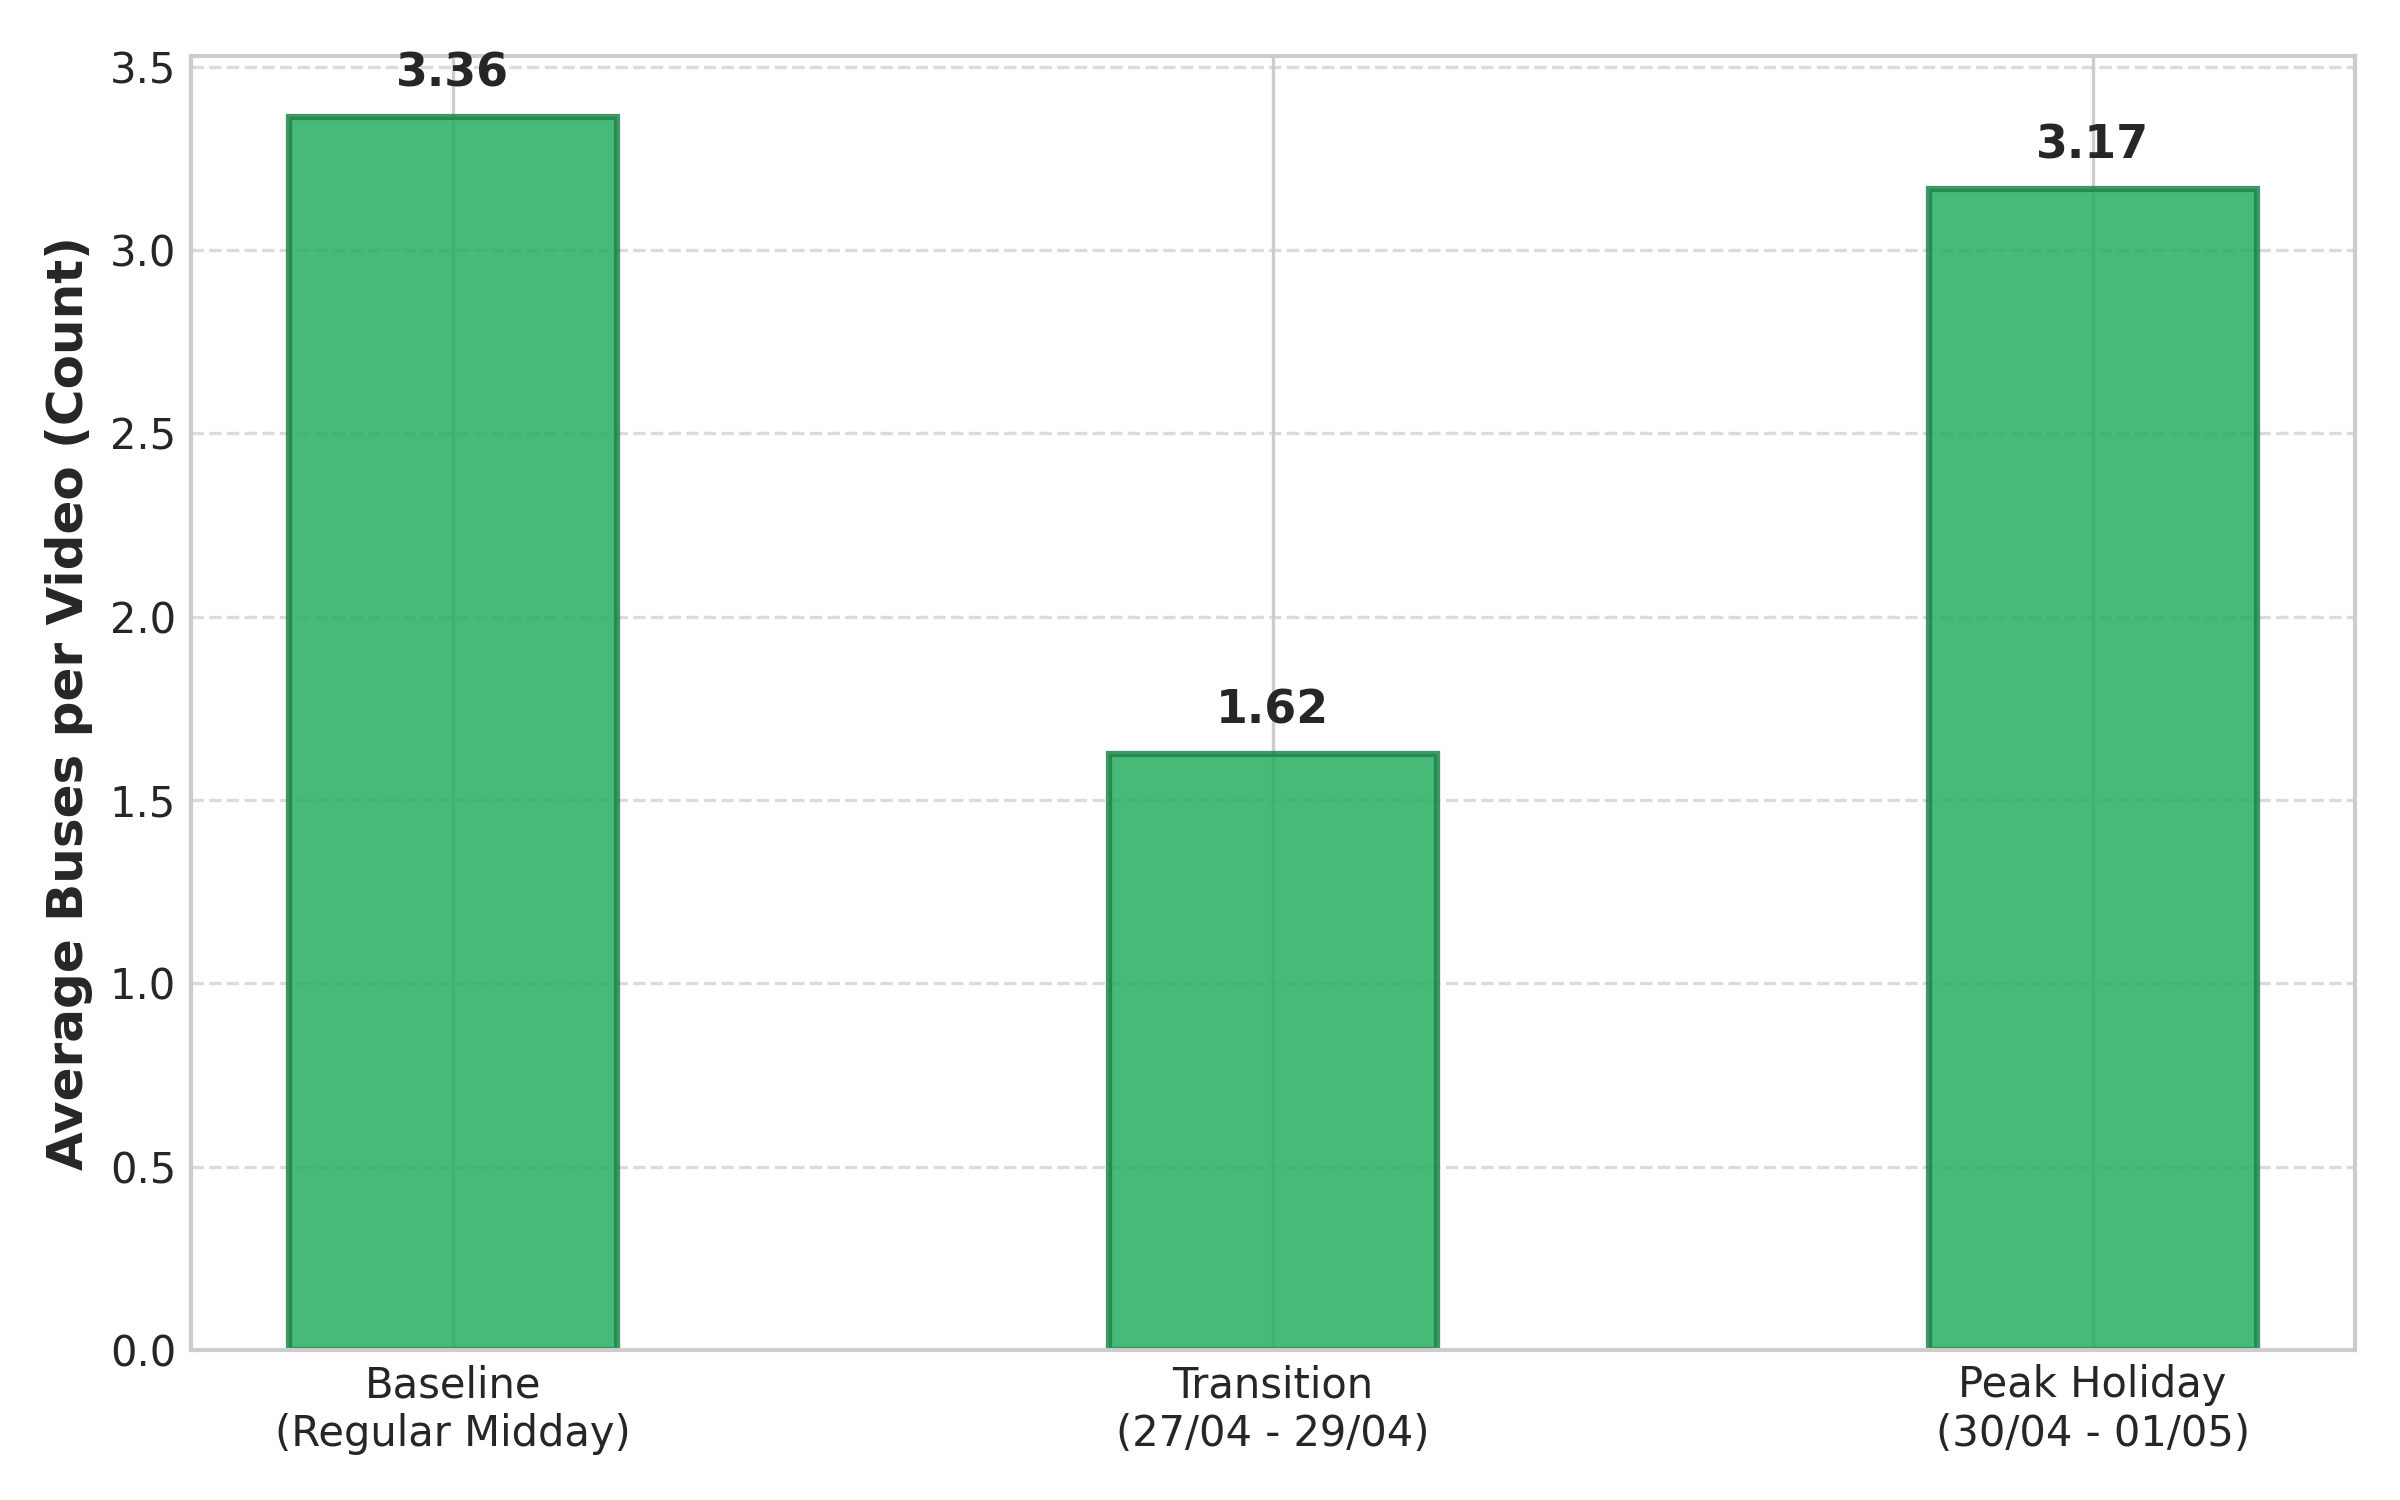
\includegraphics[keepaspectratio,alt={Distribution temporelle de la flotte d'autobus publics à Sao Bien}]{images/bus_distribution.png}}
\caption{Distribution temporelle de la flotte d'autobus publics à Sao
Bien}
\end{figure}

\paragraph{Caractérisation des profils empiriques de trafic (Baselines
et Holiday
Reversal)}\label{caractuxe9risation-des-profils-empiriques-de-trafic-baselines-et-holiday-reversal}

La campagne de mesures a collecté 72 enregistrements unitaires de 10
minutes entre le 14 avril et le 7 mai 2026. L'analyse a été menée en
deux temps. D'une part, un audit initial sur une plage de référence de 3
heures a permis d'étalonner l'erreur de classification de YOLOv8 et de
définir des baselines préliminaires de trafic (avec un flux moyen de
124,4 véhicules en Midday et 214,5 véhicules en Rush Hour). D'autre
part, la consolidation de notre campagne de mesures sur 72
enregistrements unitaires a permis d'affiner ces profils sous forme de
quatre scénarios empiriques de référence servant de conditions aux
limites pour les runs de micro-simulation physique.

\subparagraph{Le Profil de Ligne de Base (Regular Midday
Baseline)}\label{le-profil-de-ligne-de-base-regular-midday-baseline}

Calculé sur 58 observations stables lors des heures creuses de la
mi-journée (11h00 - 13h00) hors jours fériés, il caractérise un
écoulement fluide :

\begin{itemize}
\tightlist
\item
  \textbf{Volume moyen total (excluant les bus) :} \textbf{134,10
  véhicules par tranche de 10 minutes} (124,4 dans la baseline d'audit
  initiale).
\item
  \textbf{Répartition modale :}

  \begin{itemize}
  \tightlist
  \item
    \emph{Motorcycles (deux-roues) :} \textbf{67,97 unités}
    (\textbf{50,7 \%}). Le deux-roues reste le mode de transport
    dominant à Hanoï.
  \item
    \emph{Standard Cars (ICE) :} \textbf{30,38 unités} (\textbf{22,7
    \%}).
  \item
    \emph{Electric Vehicles (EV) :} \textbf{35,74 unités} (\textbf{26,7
    \%}). La part élevée d'EV s'explique par la forte concentration de
    taxis GSM.
  \end{itemize}
\item
  \textbf{État cinématique :} Circulation fluide, vitesse moyenne de 35
  km/h, occupation moyenne du hub de recharge à 75 \% (9 bornes sur 12
  occupées).
\end{itemize}

\subparagraph{Tableau 4b : Répartition modale du trafic en période
régulière (Midday
Baseline)}\label{tableau-4b-ruxe9partition-modale-du-trafic-en-puxe9riode-ruxe9guliuxe8re-midday-baseline}

{\def\LTcaptype{none} % do not increment counter
\begin{longtable}[]{@{}lcc@{}}
\toprule\noalign{}
Catégorie de véhicule & Volume moyen (véh/10 min) & Part modale (\%) \\
\midrule\noalign{}
\endhead
\bottomrule\noalign{}
\endlastfoot
Deux-roues (Motorcycles) & 67,97 & 50,7 \% \\
Voitures thermiques (Standard Cars ICE) & 30,38 & 22,7 \% \\
Véhicules électriques (Electric Cars EV) & 35,74 & 26,7 \% \\
\textbf{Total moyen} & \textbf{134,10} & \textbf{100,0 \%} \\
\end{longtable}
}

\begin{figure}
\centering
\pandocbounded{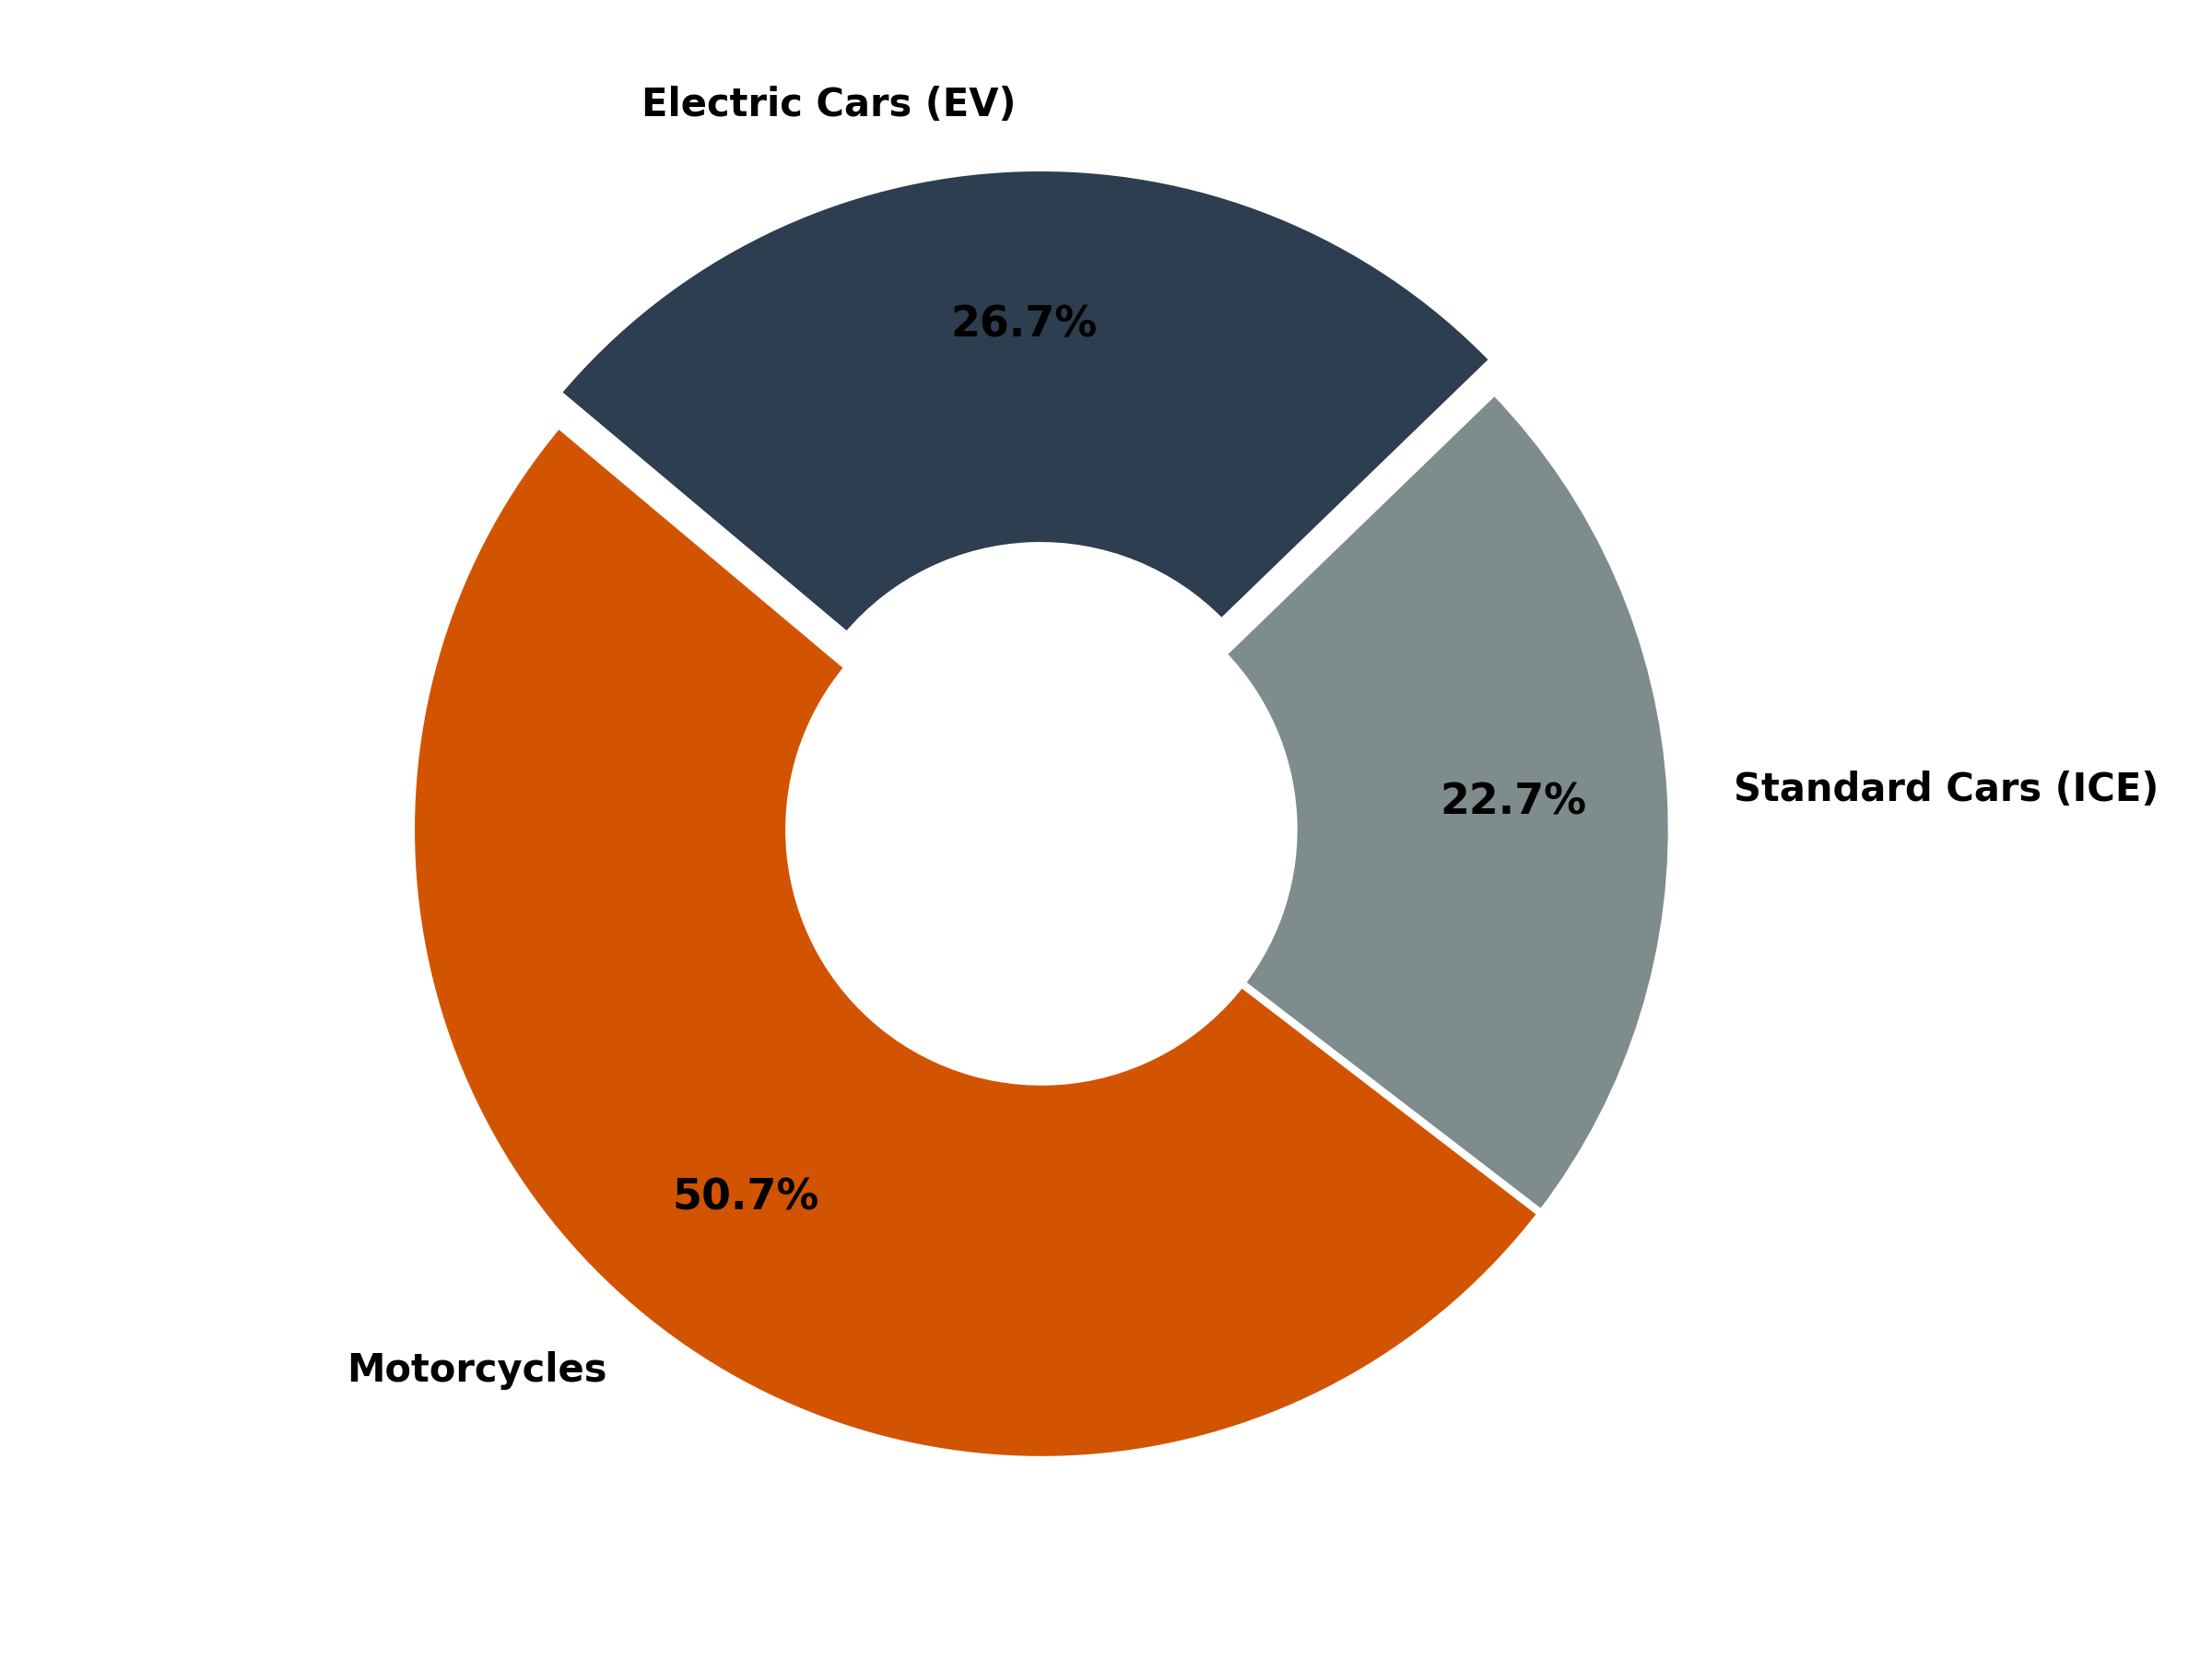
\includegraphics[keepaspectratio,alt={Structure modale du trafic en période régulière de mi-journée (Regular Midday) - Répartition à Sao Bien}]{images/traffic_composition_pie.png}}
\caption{Structure modale du trafic en période régulière de mi-journée
(Regular Midday) - Répartition à Sao Bien}
\end{figure}

\subparagraph{Le Profil d'Heure de Pointe (Regular Evening
Peak)}\label{le-profil-dheure-de-pointe-regular-evening-peak}

Modélise la surpression cinématique observée en fin de journée (17h00 -
18h00), marquée par le retour des travailleurs :

\begin{itemize}
\tightlist
\item
  \textbf{Volume moyen total (excluant les bus) :} \textbf{227,67
  véhicules par tranche de 10 minutes} (214,5 dans l'audit initial),
  soit une hausse de \textbf{70 \%} par rapport à la baseline.
\item
  \textbf{Répartition modale :}

  \begin{itemize}
  \tightlist
  \item
    \emph{Motorcycles (deux-roues) :} \textbf{143,06 unités}
    (\textbf{62,8 \%}). La part des motos s'accroit, accentuant les
    frictions inter-voies.
  \item
    \emph{Standard Cars (ICE) :} \textbf{34,44 unités} (\textbf{15,1
    \%}).
  \item
    \emph{Electric Vehicles (EV) :} \textbf{50,17 unités} (\textbf{22,0
    \%}).
  \end{itemize}
\item
  \textbf{État cinématique :} Apparition de congestions localisées et
  baisse des vitesses.
\end{itemize}

\subparagraph{Tableau 4c : Répartition modale du trafic en heure de
pointe régulière (Regular Evening
Peak)}\label{tableau-4c-ruxe9partition-modale-du-trafic-en-heure-de-pointe-ruxe9guliuxe8re-regular-evening-peak}

{\def\LTcaptype{none} % do not increment counter
\begin{longtable}[]{@{}lcc@{}}
\toprule\noalign{}
Catégorie de véhicule & Volume moyen (véh/10 min) & Part modale (\%) \\
\midrule\noalign{}
\endhead
\bottomrule\noalign{}
\endlastfoot
Deux-roues (Motorcycles) & 143,06 & 62,8 \% \\
Voitures thermiques (Standard Cars ICE) & 34,44 & 15,1 \% \\
Véhicules électriques (Electric Cars EV) & 50,17 & 22,0 \% \\
\textbf{Total moyen} & \textbf{227,67} & \textbf{100,0 \%} \\
\end{longtable}
}

\begin{figure}
\centering
\pandocbounded{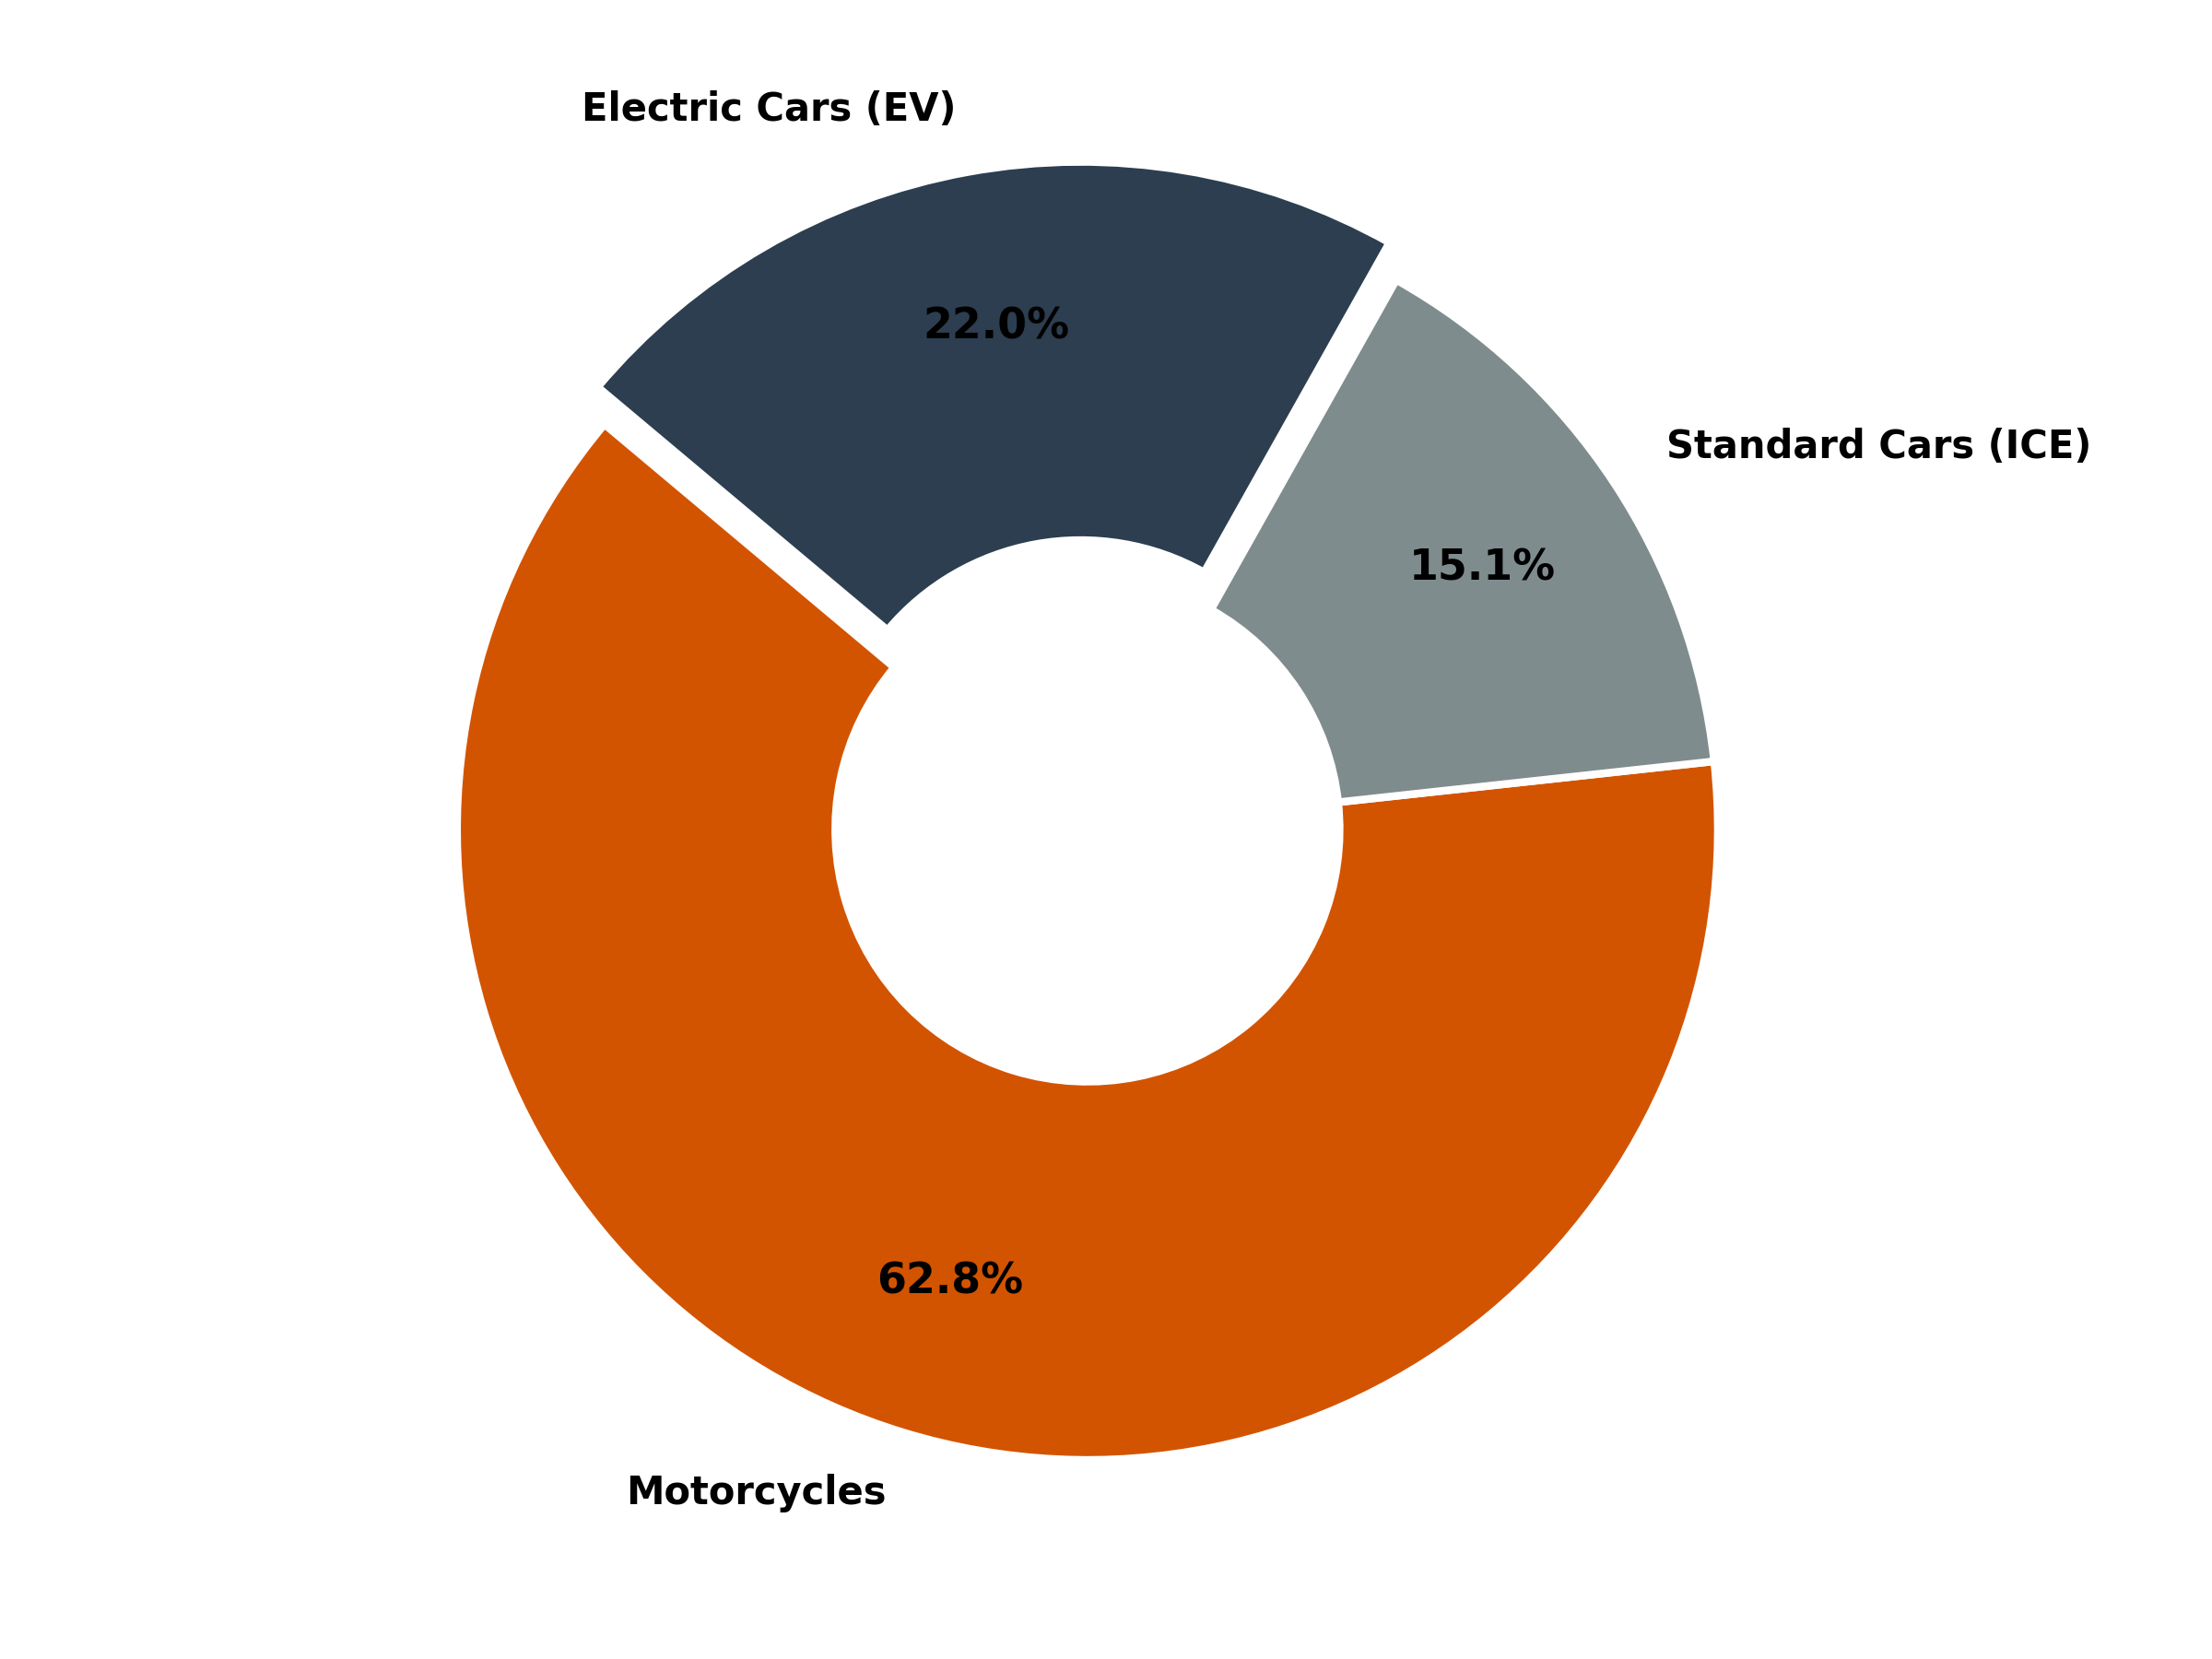
\includegraphics[keepaspectratio,alt={Structure modale du trafic en heure de pointe de soirée (Evening Rush Hour) - Répartition à Sao Bien}]{images/traffic_composition_rush_pie.png}}
\caption{Structure modale du trafic en heure de pointe de soirée
(Evening Rush Hour) - Répartition à Sao Bien}
\end{figure}

\subparagraph{Le Profil de Rupture : Le phénomène de ``Holiday
Reversal''}\label{le-profil-de-rupture-le-phuxe9nomuxe8ne-de-holiday-reversal}

Les mesures enregistrées lors des fêtes nationales du 30 avril et du 1er
mai ont révélé une anomalie comportementale majeure. Le volume de trafic
global diminue légèrement à \textbf{117,17 véhicules par 10 minutes} (en
raison du départ d'une partie des résidents hors de la ville), mais la
répartition modale subit une inversion complète :

\begin{itemize}
\tightlist
\item
  \emph{Motorcycles (deux-roues) :} \textbf{46,50 unités} (\textbf{39,7
  \%}). Baisse de plus de 10 points de pourcentage.
\item
  \emph{Standard Cars (ICE) :} \textbf{23,83 unités} (\textbf{20,3 \%}).
\item
  \emph{Electric Vehicles (EV) :} \textbf{46,83 unités} (\textbf{40,0
  \%}).
\end{itemize}

Sur le segment des véhicules à 4 roues (ICE + EV), \textbf{les véhicules
électriques représentent 66,3 \% de la flotte active}. Ce comportement
s'explique par l'afflux massif de familles visitant le Vincom Mega Mall
à bord de taxis GSM électriques et de SUV électriques individuels. Cette
inversion modale entraînera une saturation instantanée du hub de
recharge (100 \% d'occupation) et la formation de files d'attente
bloquantes sur la voirie.

\subparagraph{Tableau 4d : Comparaison de la structure de trafic :
Semaine Régulière vs Période de Vacances (Holiday
Reversal)}\label{tableau-4d-comparaison-de-la-structure-de-trafic-semaine-ruxe9guliuxe8re-vs-puxe9riode-de-vacances-holiday-reversal}

{\def\LTcaptype{none} % do not increment counter
\begin{longtable}[]{@{}
  >{\raggedright\arraybackslash}p{(\linewidth - 8\tabcolsep) * \real{0.1667}}
  >{\centering\arraybackslash}p{(\linewidth - 8\tabcolsep) * \real{0.2083}}
  >{\centering\arraybackslash}p{(\linewidth - 8\tabcolsep) * \real{0.2083}}
  >{\centering\arraybackslash}p{(\linewidth - 8\tabcolsep) * \real{0.2083}}
  >{\centering\arraybackslash}p{(\linewidth - 8\tabcolsep) * \real{0.2083}}@{}}
\toprule\noalign{}
\begin{minipage}[b]{\linewidth}\raggedright
Catégorie de véhicule
\end{minipage} & \begin{minipage}[b]{\linewidth}\centering
Volume Baseline (Midi régulier)
\end{minipage} & \begin{minipage}[b]{\linewidth}\centering
Part Baseline (\%)
\end{minipage} & \begin{minipage}[b]{\linewidth}\centering
Volume Holiday (Midi vacances)
\end{minipage} & \begin{minipage}[b]{\linewidth}\centering
Part Holiday (\%)
\end{minipage} \\
\midrule\noalign{}
\endhead
\bottomrule\noalign{}
\endlastfoot
Deux-roues (Motorcycles) & 67,97 & 50,7 \% & 46,50 & 39,7 \% \\
Voitures thermiques (Standard Cars ICE) & 30,38 & 22,7 \% & 23,83 & 20,3
\% \\
Véhicules électriques (Electric Cars EV) & 35,74 & 26,7 \% & 46,83 &
40,0 \% \\
\textbf{Total} & \textbf{134,10} & \textbf{100,0 \%} & \textbf{117,17} &
\textbf{100,0 \%} \\
\end{longtable}
}

\begin{figure}
\centering
\pandocbounded{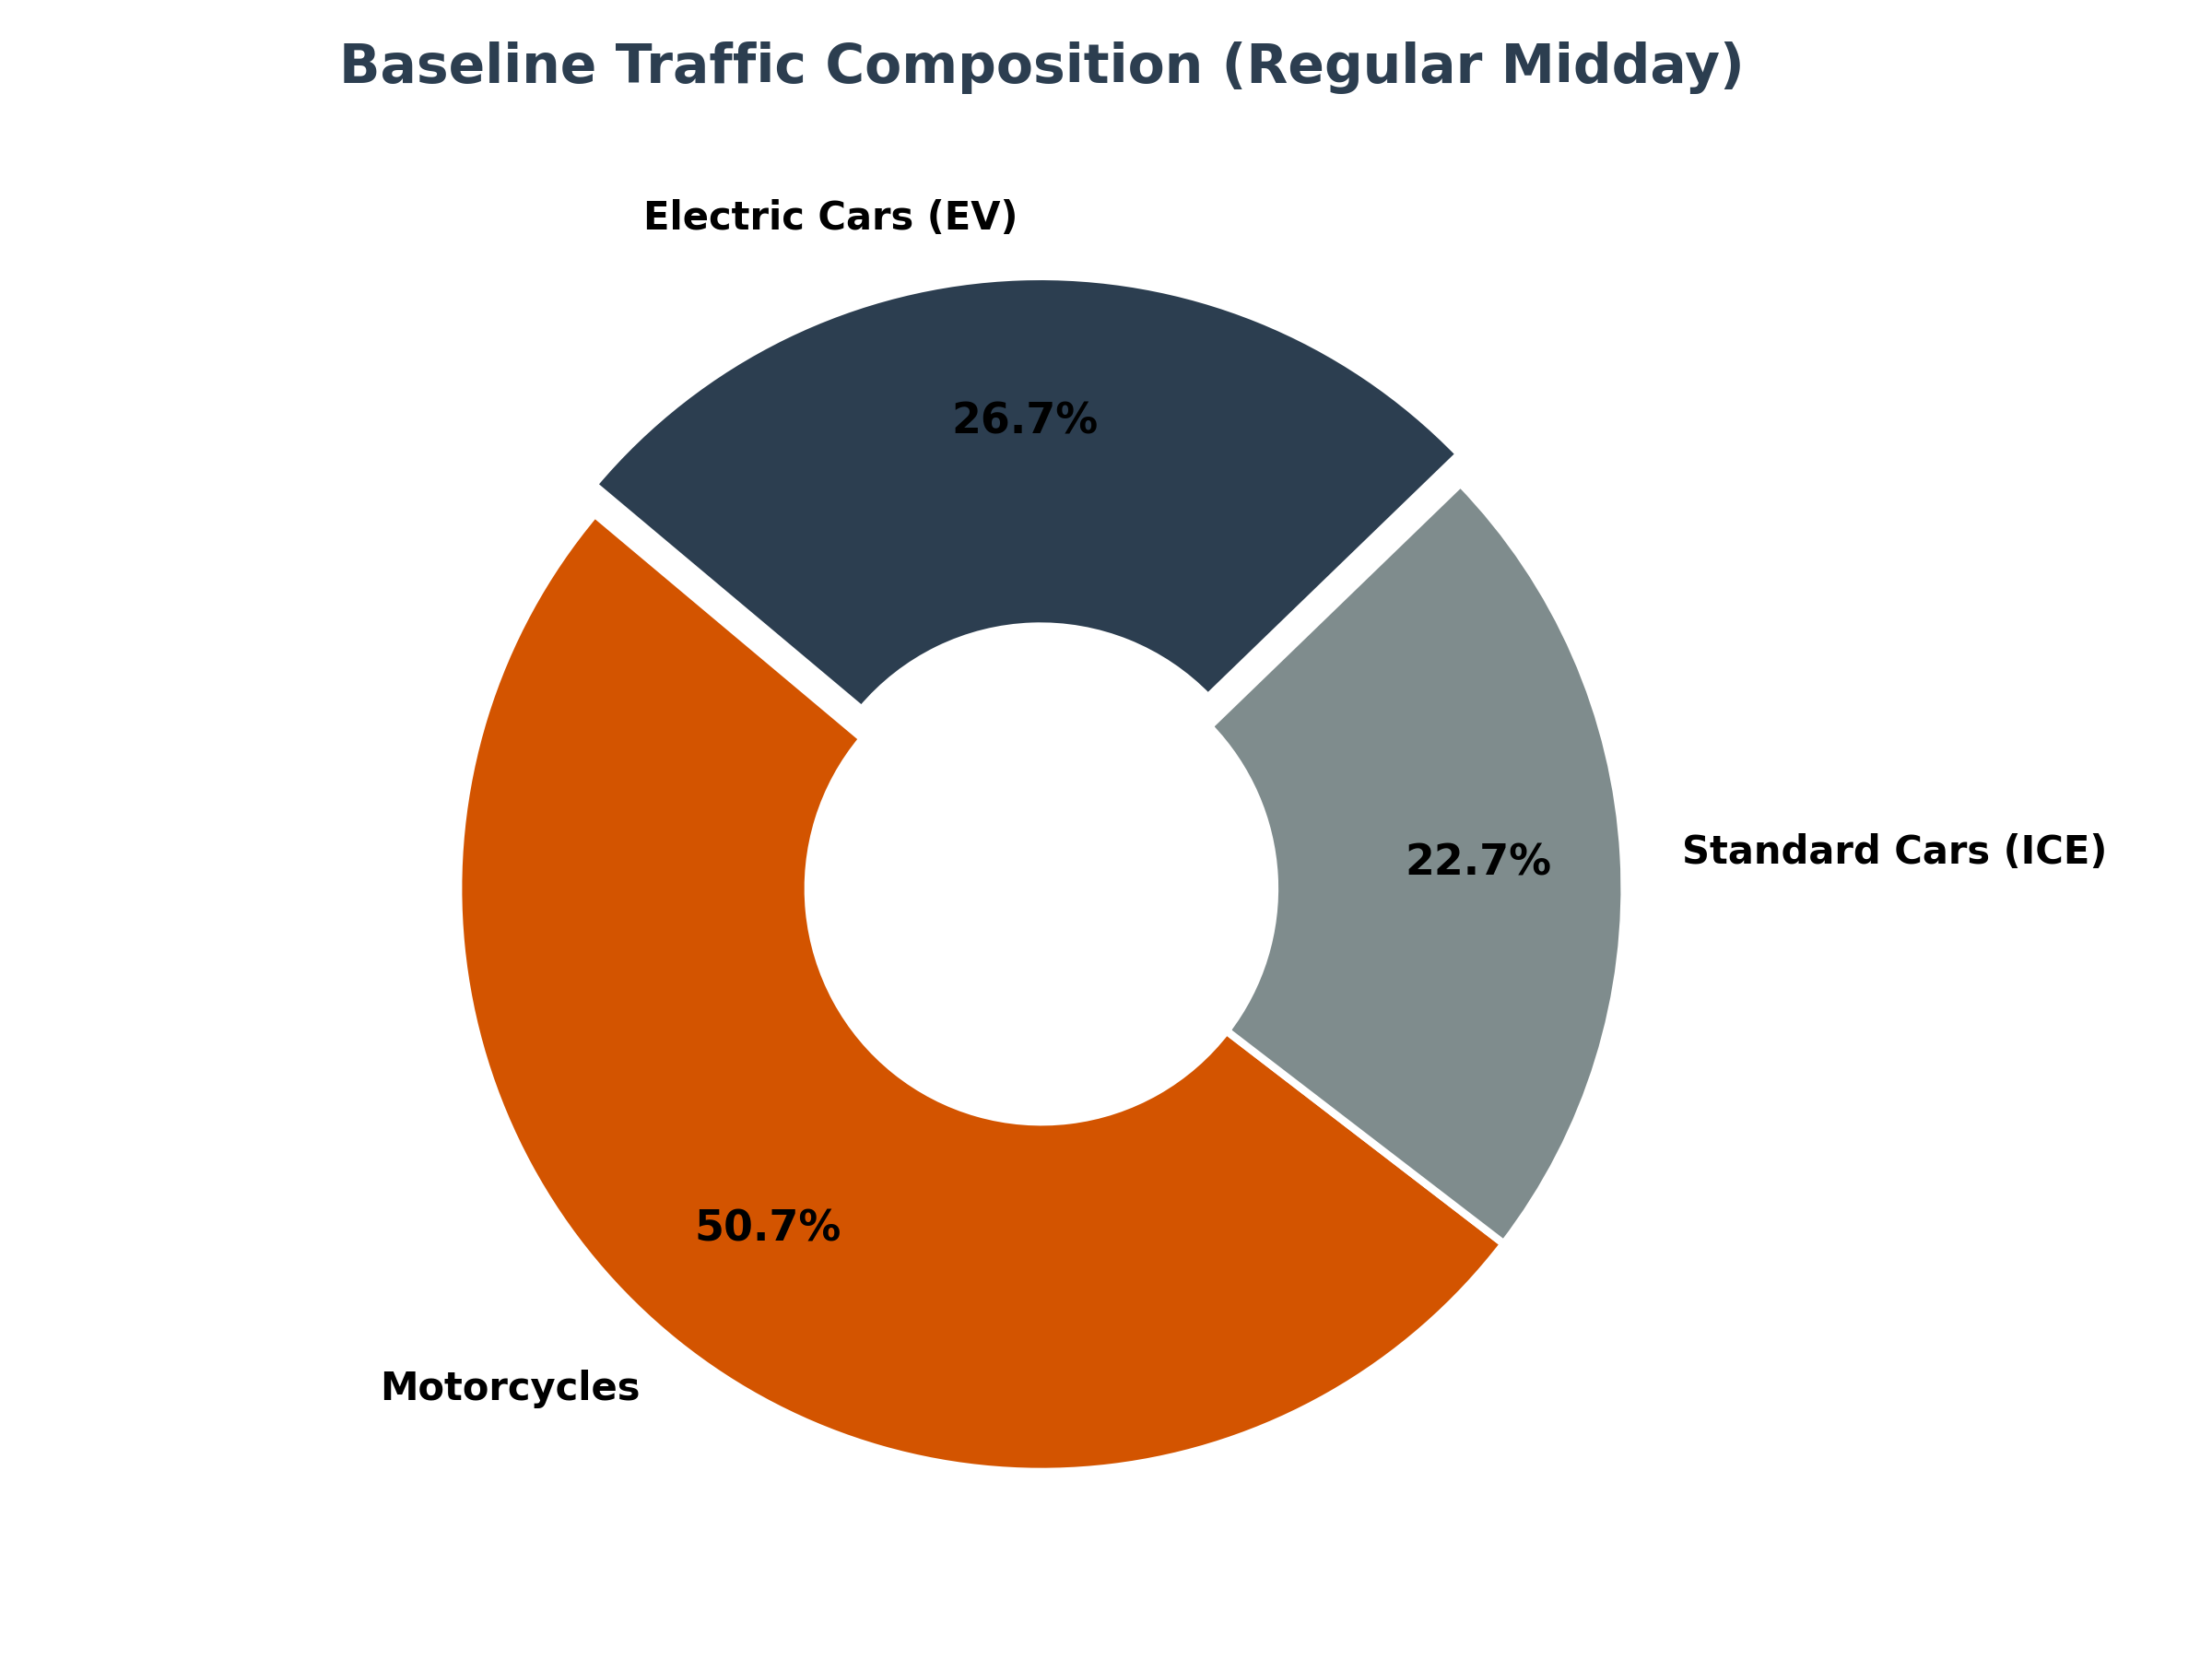
\includegraphics[keepaspectratio,alt={Répartition modale comparée du fluide de trafic (Midi Régulier vs Holiday Reversal) lors de la campagne de mesures}]{images/traffic_composition_pie-Hanoi.png}}
\caption{Répartition modale comparée du fluide de trafic (Midi Régulier
vs Holiday Reversal) lors de la campagne de mesures}
\end{figure}

\subparagraph{La Période de Transition Pré-Vacances (27 - 29
Avril)}\label{la-puxe9riode-de-transition-pruxe9-vacances-27---29-avril}

Un régime transitoire de montée en charge avec un volume moyen de
\textbf{123,83 véhicules par 10 minutes} :

\begin{itemize}
\tightlist
\item
  \emph{Motorcycles :} \textbf{58,00 unités} (\textbf{46,8 \%}).
\item
  \emph{Standard Cars (ICE) :} \textbf{32,33 unités} (\textbf{26,1 \%}).
\item
  \emph{Electric Vehicles :} \textbf{33,50 unités} (\textbf{27,1 \%}).
\end{itemize}

\begin{figure}
\centering
\pandocbounded{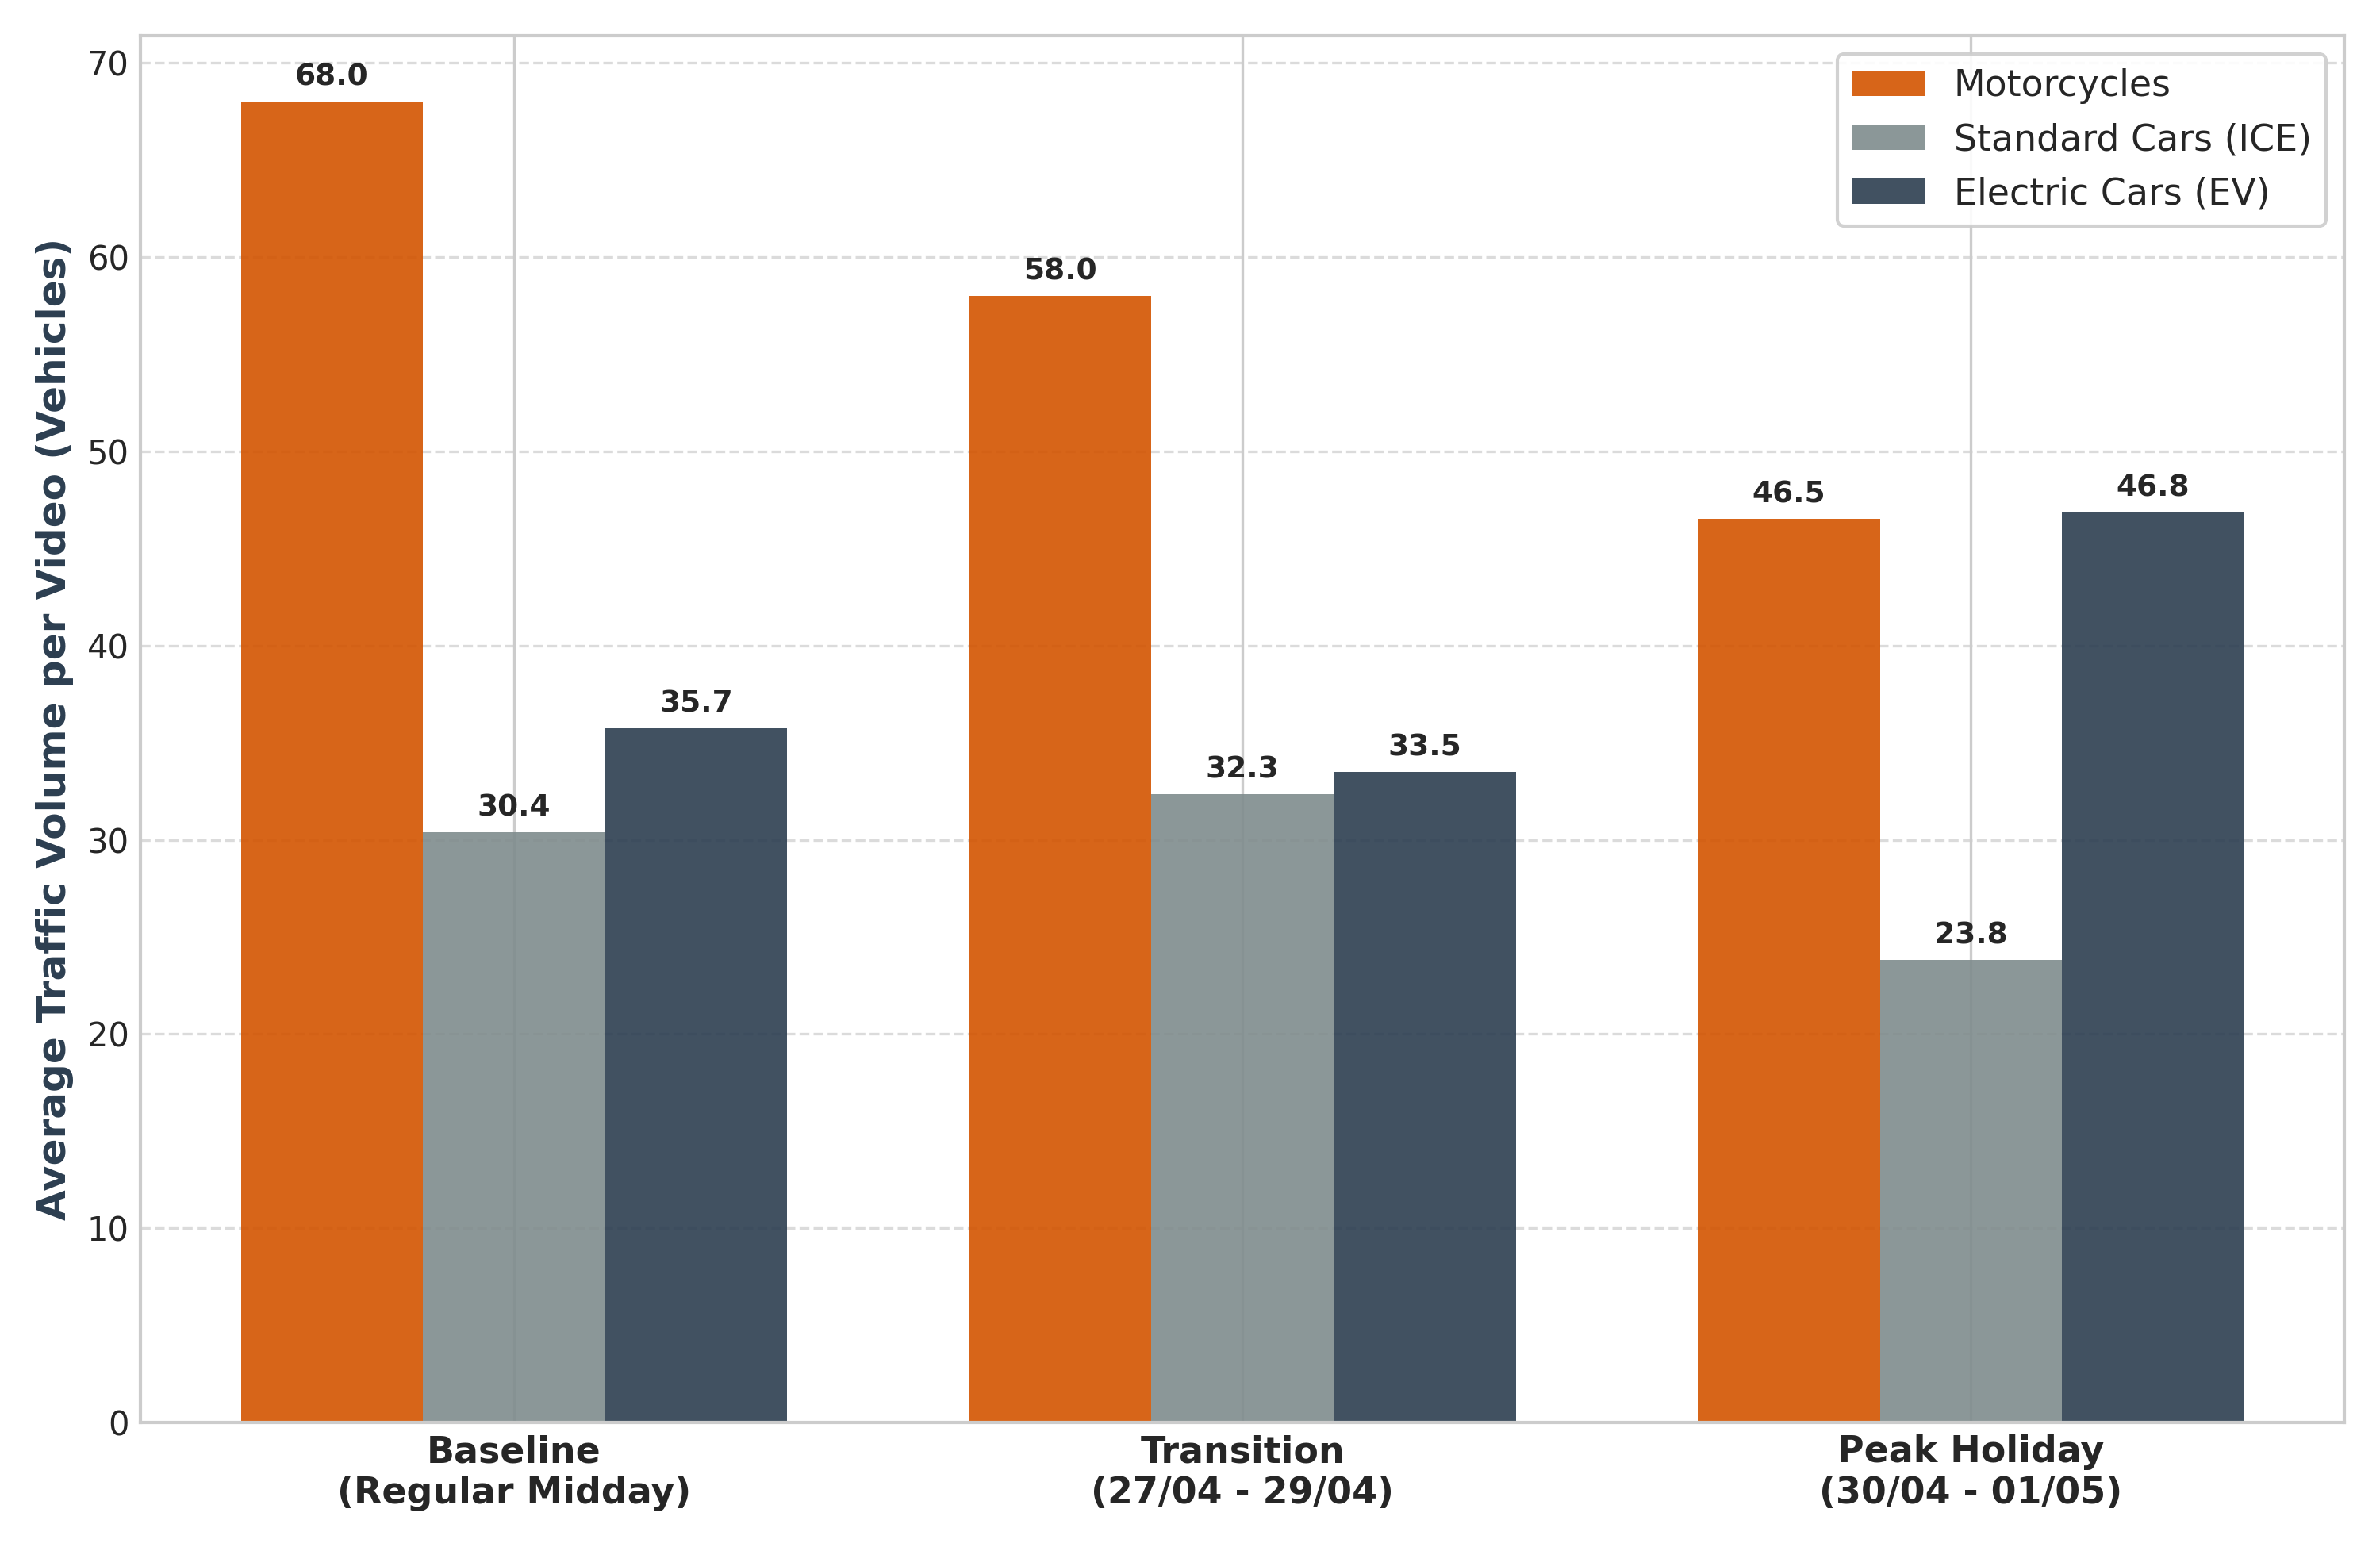
\includegraphics[keepaspectratio,alt={Évolution de la structure modale du trafic selon les périodes (Midi régulier, Transition, Vacances)}]{images/vacation_comparison.png}}
\caption{Évolution de la structure modale du trafic selon les périodes
(Midi régulier, Transition, Vacances)}
\end{figure}

\begin{figure}
\centering
\pandocbounded{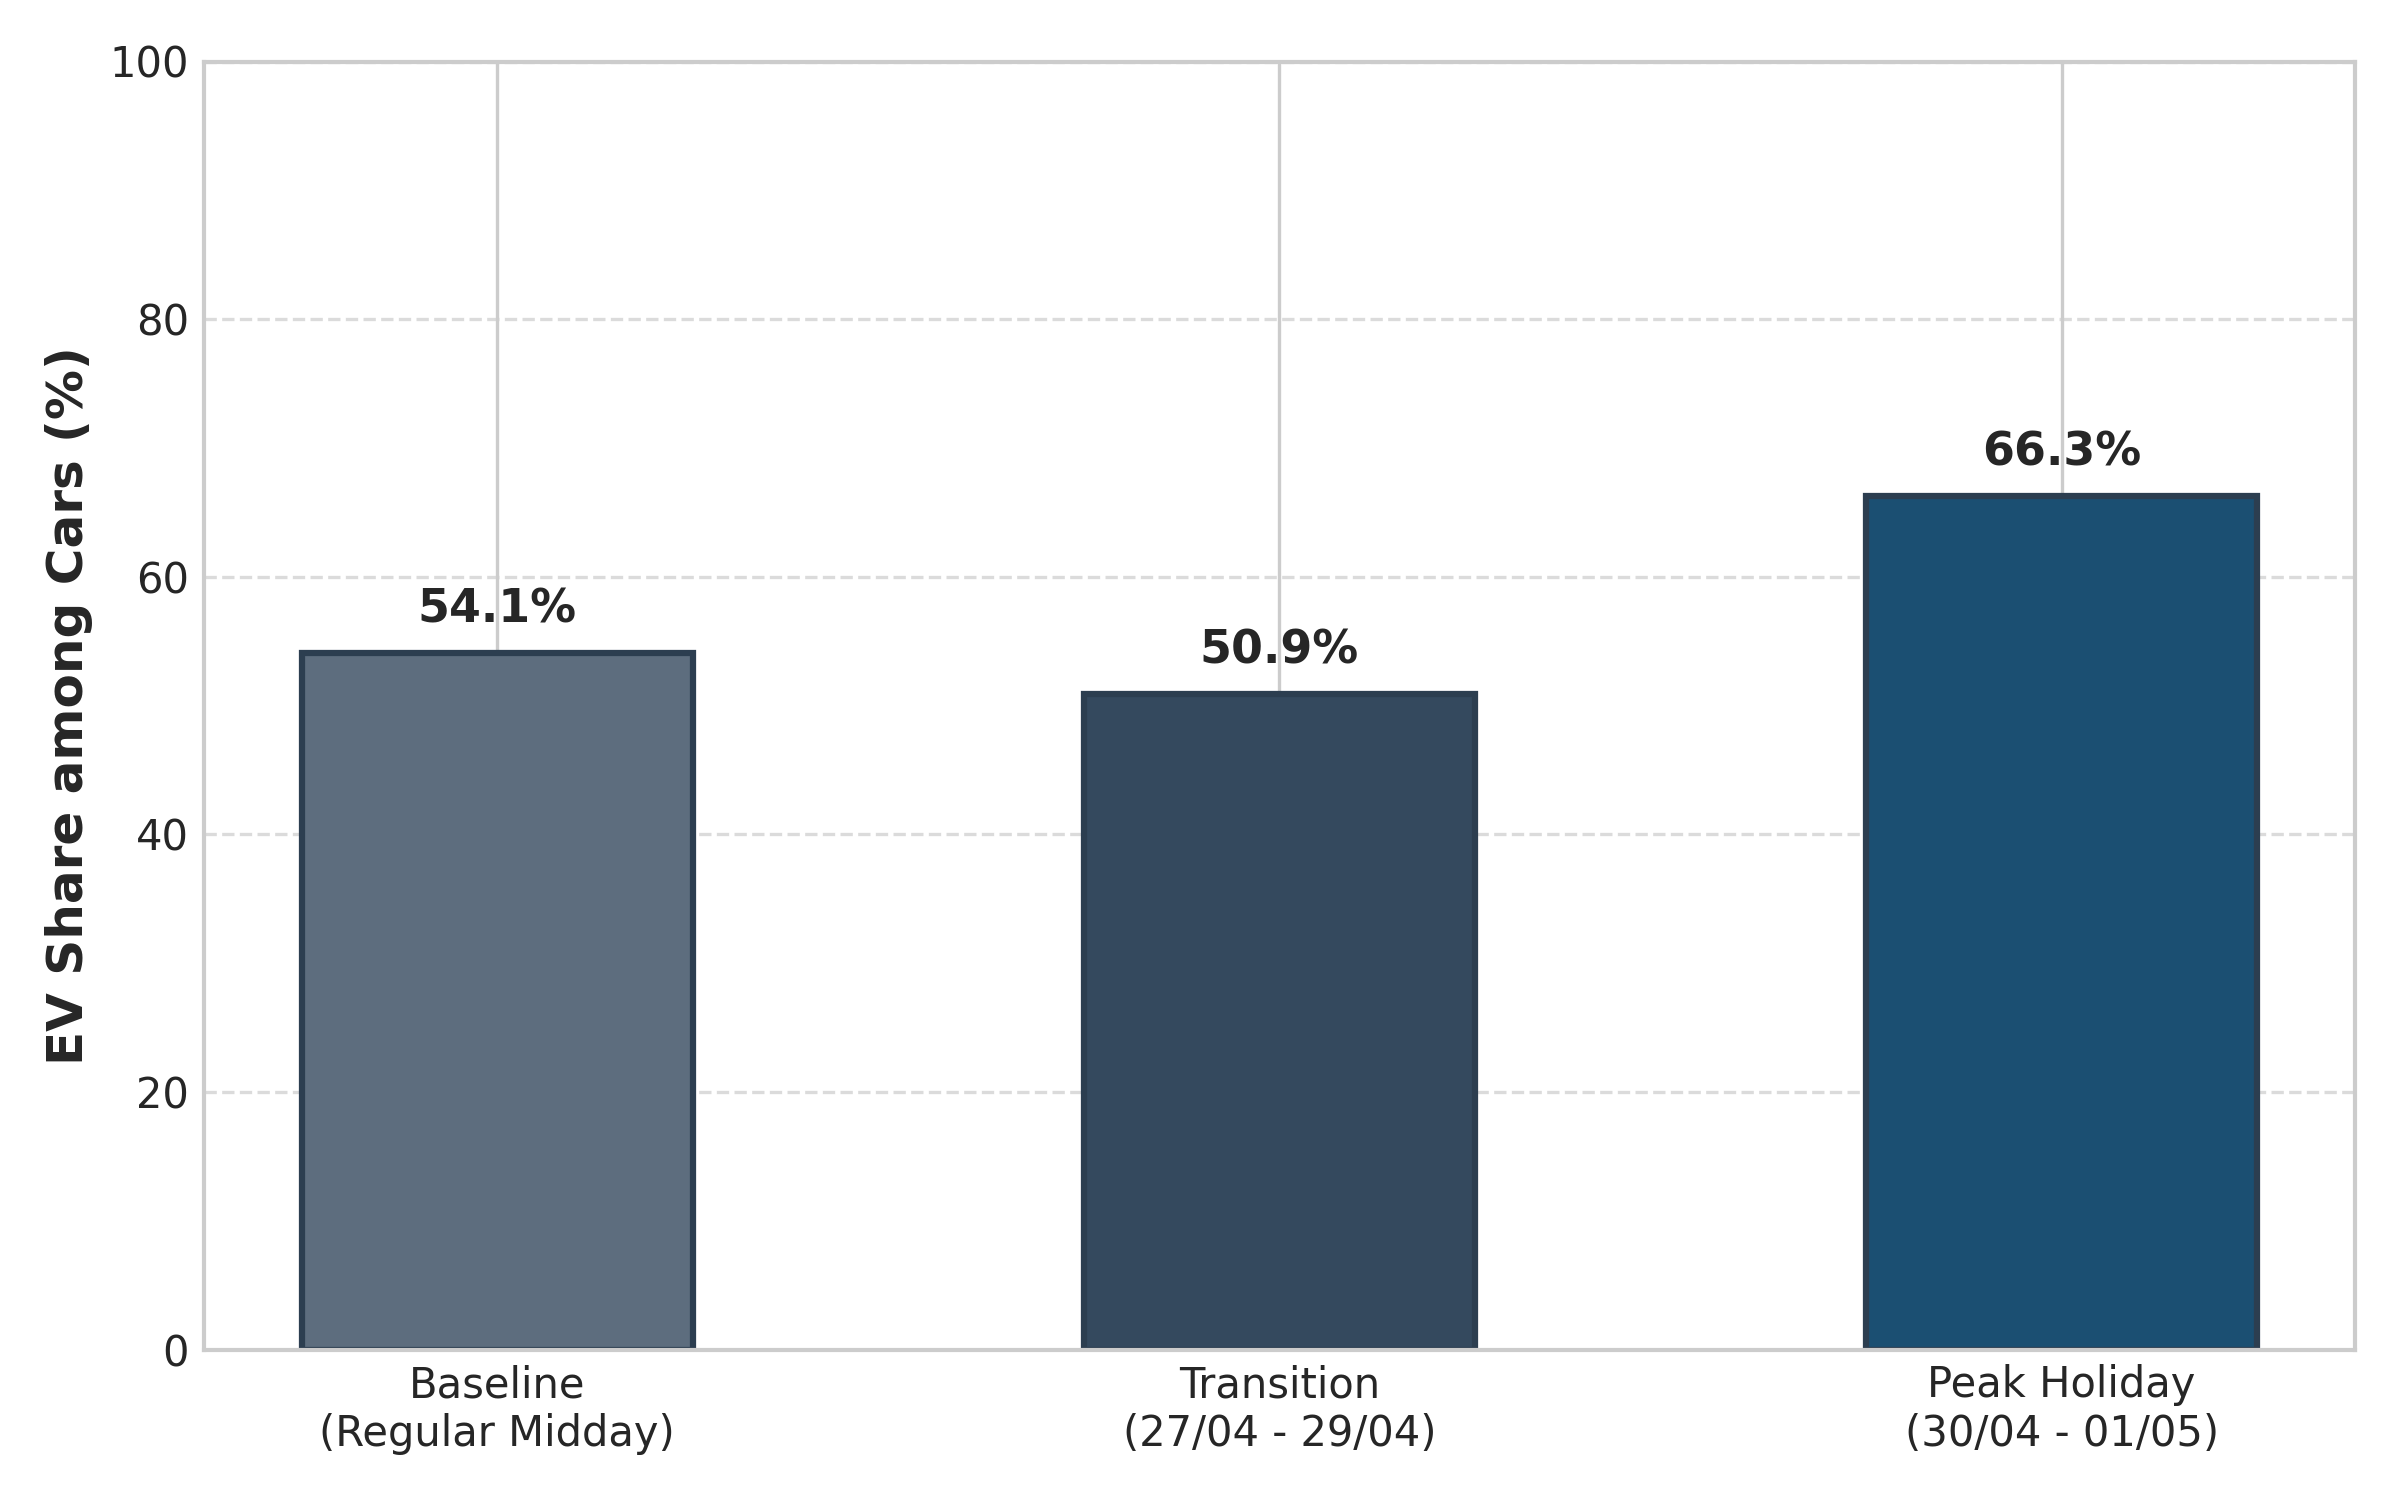
\includegraphics[keepaspectratio,alt={Taux de pénétration des véhicules électriques au sein du segment des quatre roues}]{images/ev_distribution_bar.png}}
\caption{Taux de pénétration des véhicules électriques au sein du
segment des quatre roues}
\end{figure}

\begin{figure}
\centering
\pandocbounded{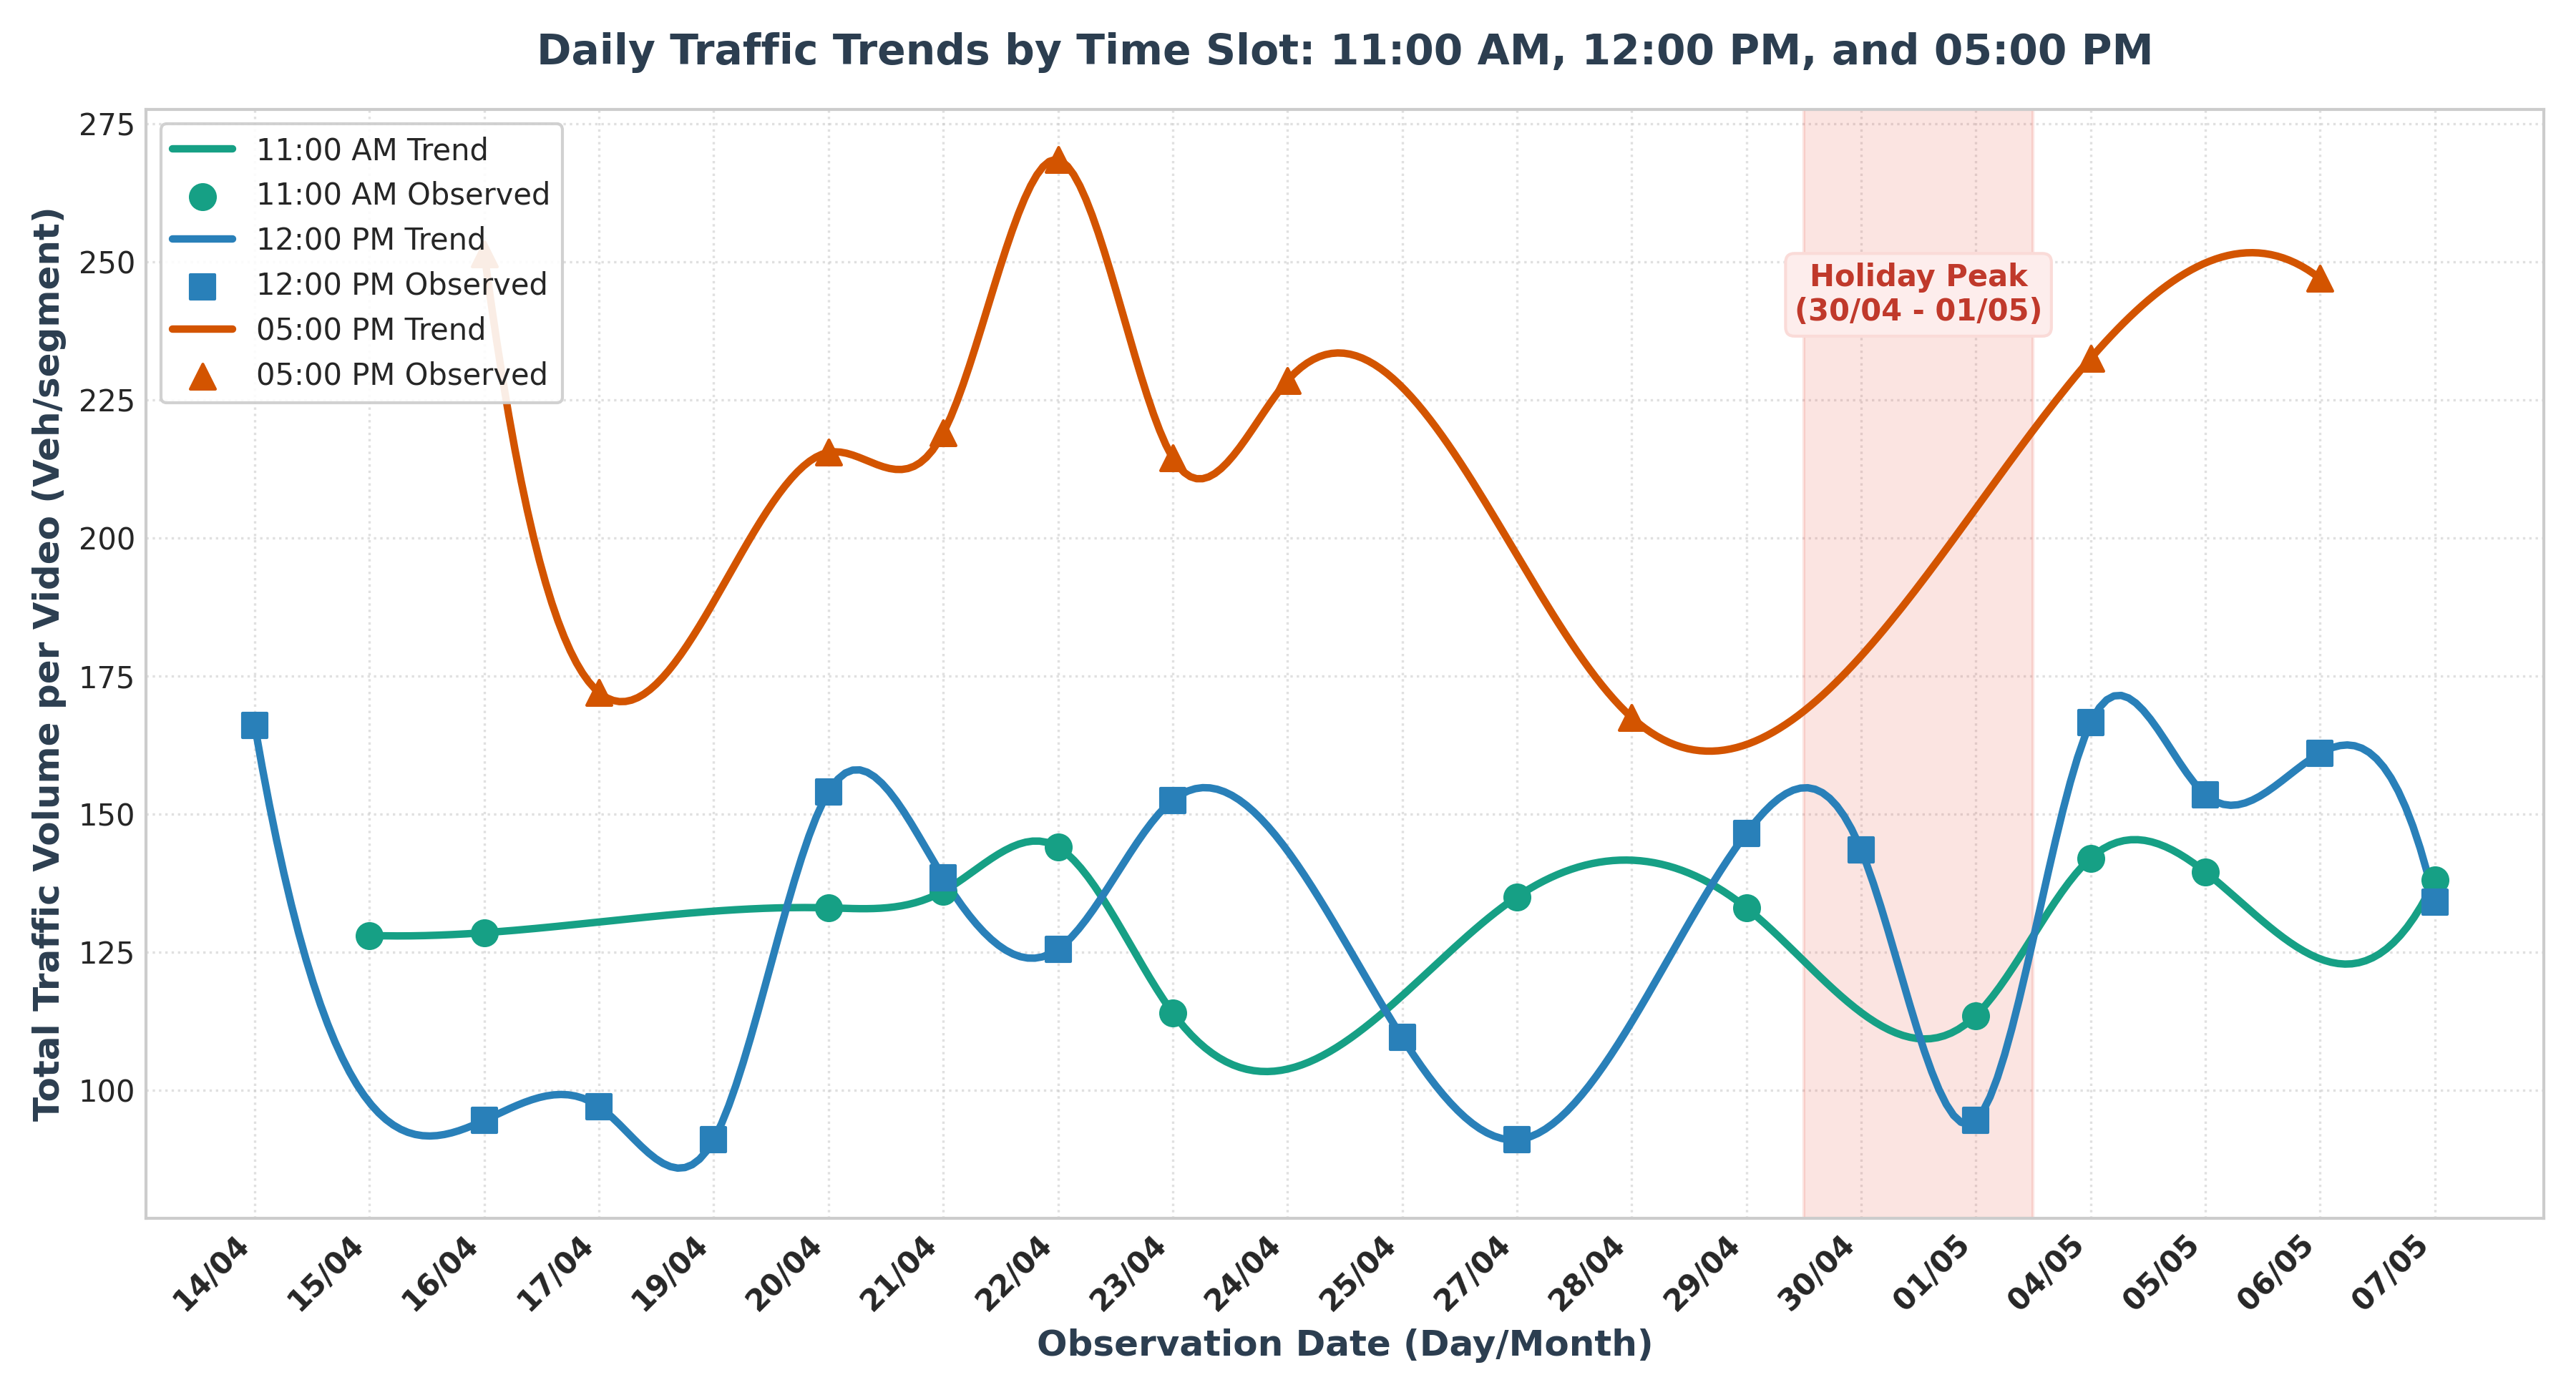
\includegraphics[keepaspectratio,alt={Évolution journalière des volumes de trafic par créneaux horaires (11h00, 12h00, 17h00) durant la campagne de mesures à Sao Bien (Hanoï)}]{images/daily_timeline_by_hour.png}}
\caption{Évolution journalière des volumes de trafic par créneaux
horaires (11h00, 12h00, 17h00) durant la campagne de mesures à Sao Bien
(Hanoï)}
\end{figure}

\pandocbounded{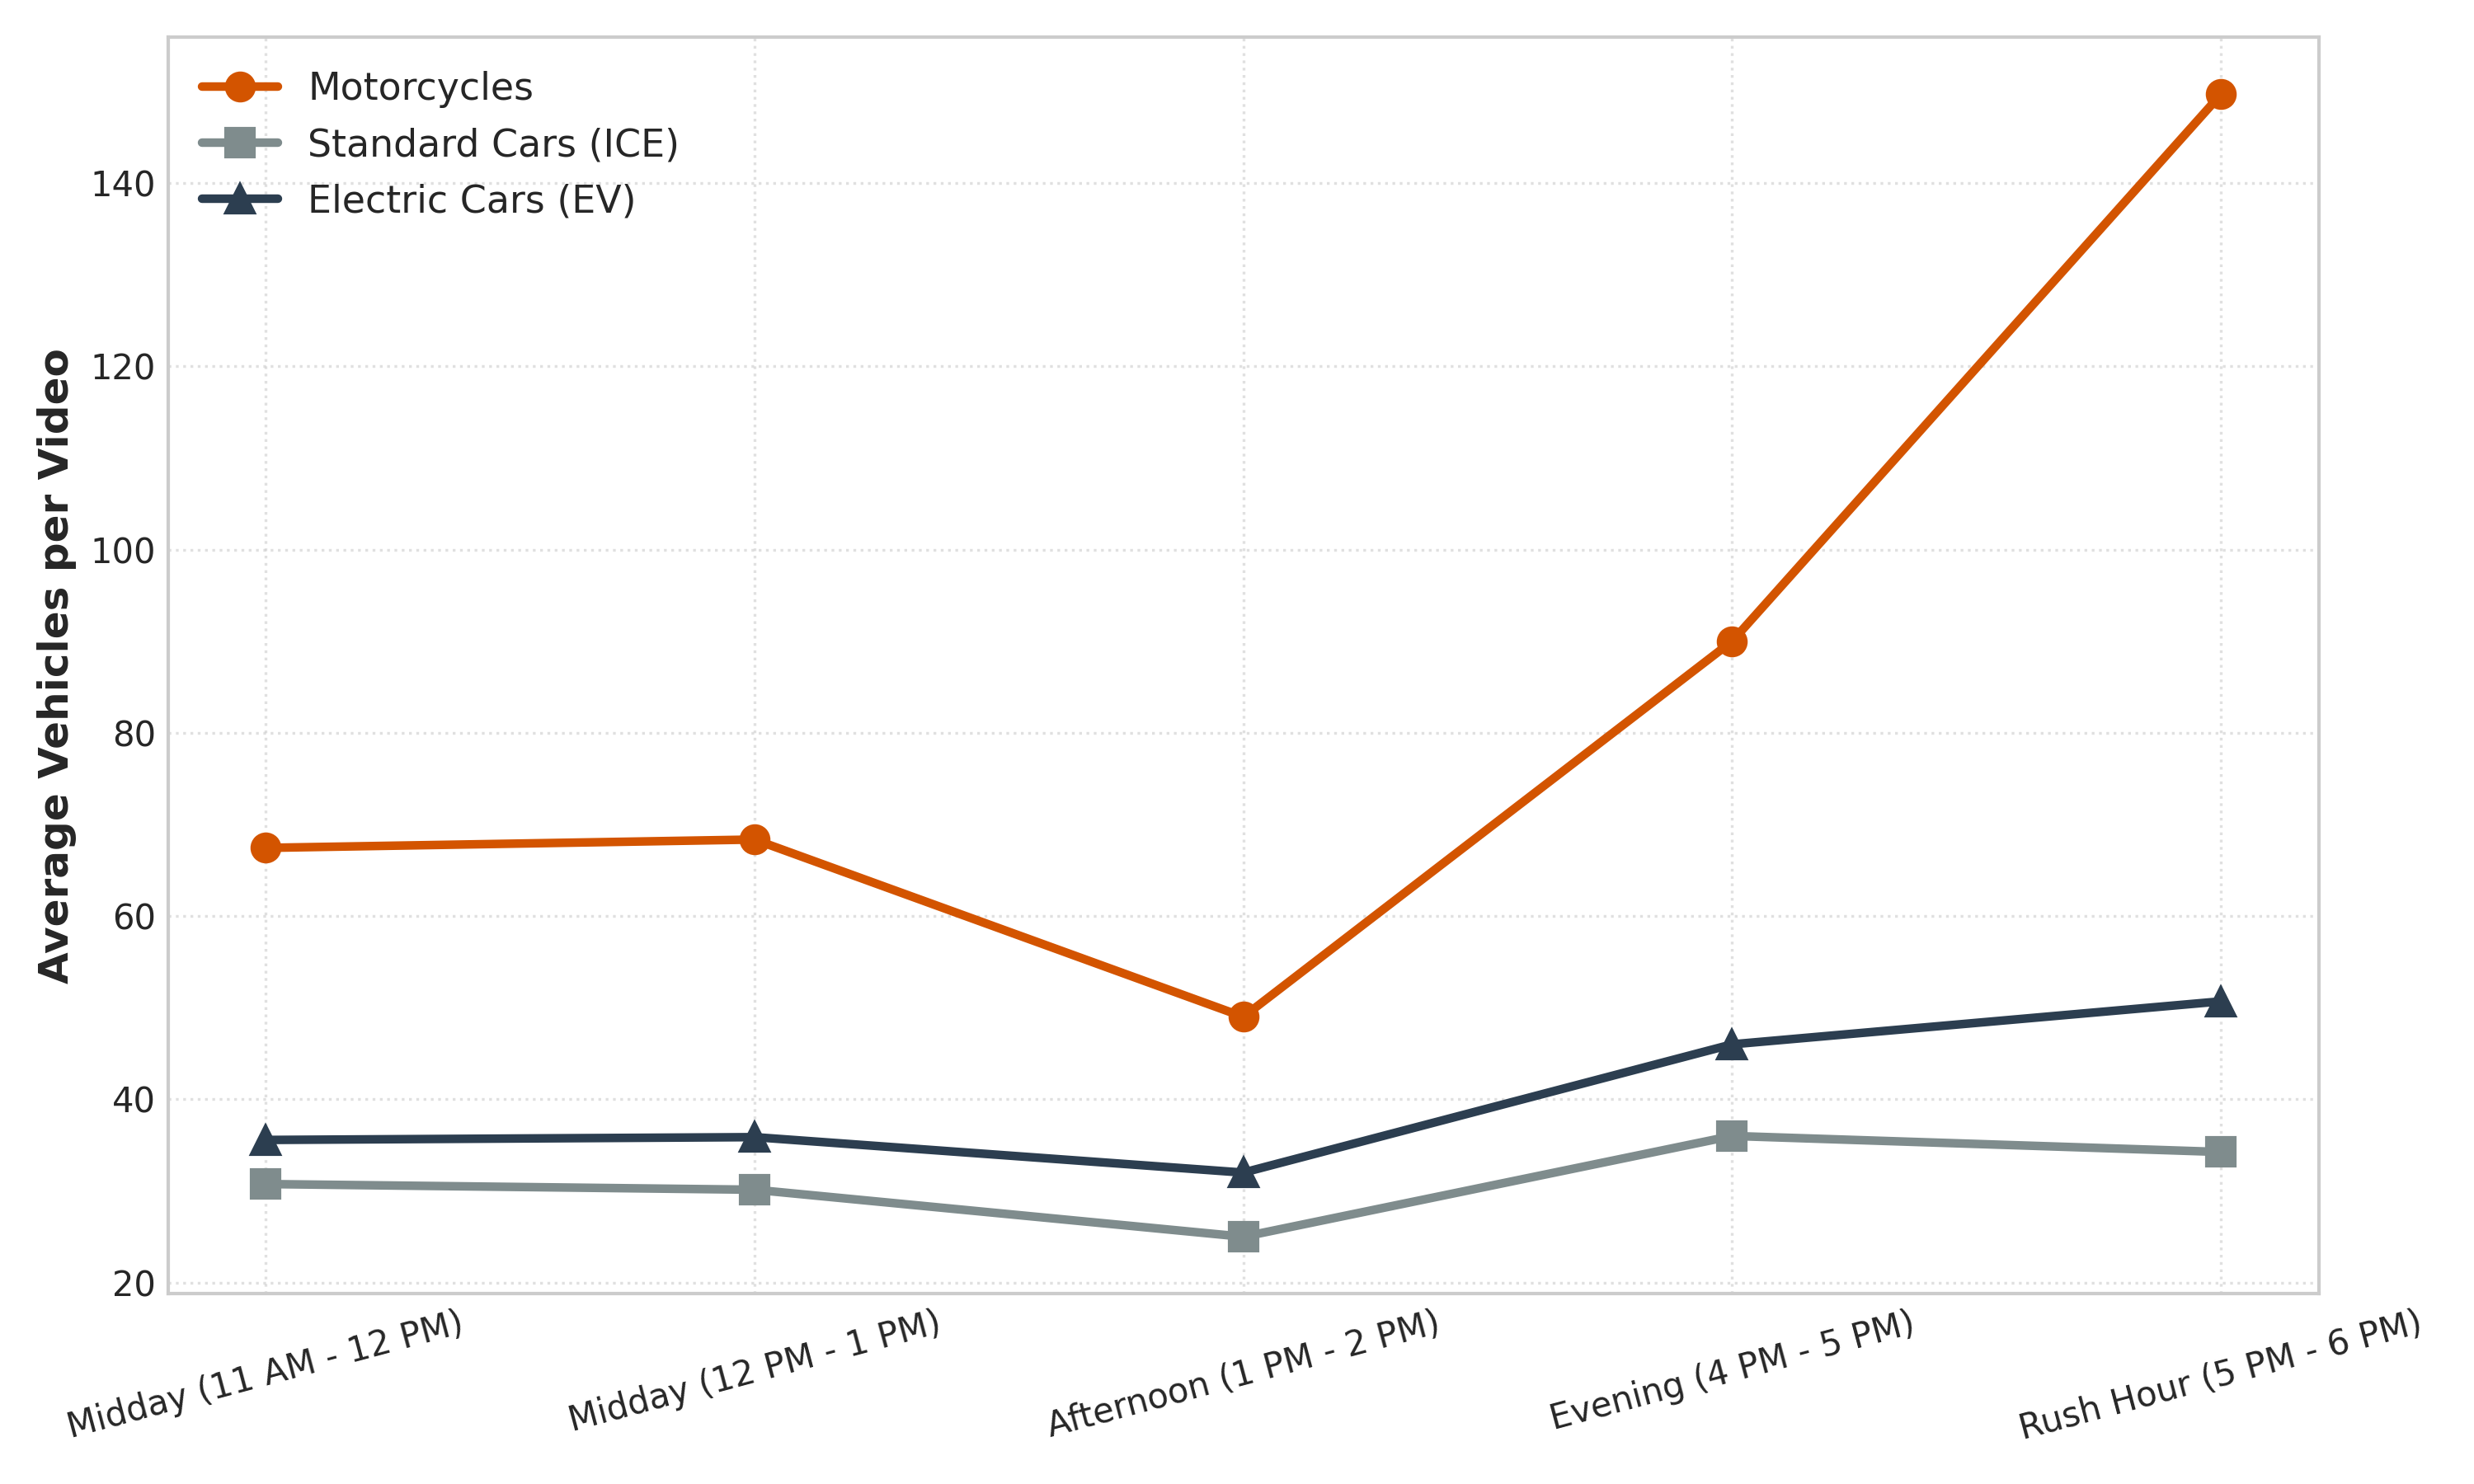
\includegraphics[keepaspectratio,alt={Profil d'intensité horaire global du trafic sur l'avenue Sao Bien}]{images/hourly_peaks.png}}
\#\#\#\# Modélisation stochastique de la recharge et initialisation par
Warm-Start

\subparagraph{Le modèle de temps d'arrêt stochastique (Stochastic Dwell
Time)}\label{le-moduxe8le-de-temps-darruxeat-stochastique-stochastic-dwell-time}

Pour représenter fidèlement l'impact de la station de recharge sur le
trafic, il est scientifiquement inexact de modéliser le temps de
raccordement des véhicules électriques (\emph{dwell time}) par une
valeur fixe ou une moyenne simpliste. Dans la réalité physique, la durée
d'une session de recharge est une variable stochastique complexe. Elle
dépend de la puissance nominale de la borne (150 kW DC), mais également
de la courbe de charge de la batterie régie par le système de gestion
thermique (Battery Management System - BMS), du niveau de charge initial
du véhicule à son arrivée (\(SoC_{in}\)) et du niveau de charge souhaité
par l'usager à son départ (\(SoC_{out}\)).

Selon les spécifications techniques de VinFast et de l'opérateur de
recharge V-Green, le cycle de charge standard pour une batterie de 42 à
80 kWh (modèles VF e34, VF8, VF9) de 10 \% à 70 \% de \(SoC\) s'établit
à \textbf{31 minutes} sous une puissance stabilisée. Au-delà de 70 \%,
la puissance de charge décroît de manière exponentielle pour préserver
l'intégrité électrochimique des cellules.

Pour intégrer cette variabilité au sein du simulateur SUMO, nous avons
développé un \textbf{Modèle de Temps d'Arrêt Stochastique} basé sur une
loi normale tronquée. La durée d'arrêt \(d\) d'un véhicule électrique
ciblé pour une session de recharge suit la loi :
\[d \sim \mathcal{N}(\mu, \sigma^2)\] calibrée selon quatre profils
opérationnels d'encombrement du hub issus de nos observations :

\begin{itemize}
\tightlist
\item
  \textbf{Profil Léger (Light) :} Modélise des recharges d'appoint
  rapides.
  \[\mu = 1050 \text{ s } (17.5 \text{ min}), \quad \sigma = 225 \text{ s } (3.75 \text{ min})\]
\item
  \textbf{Profil Modéré (Moderate) :} Calibré sur le benchmark standard
  VinFast.
  \[\mu = 2100 \text{ s } (35 \text{ min}), \quad \sigma = 300 \text{ s } (5 \text{ min})\]
\item
  \textbf{Profil Lourd (Heavy) :} Modélise les sessions de recharge
  complètes ou les ralentissements dus au partage de puissance dynamique
  (\emph{power-sharing}) entre bornes adjacentes.
  \[\mu = 3600 \text{ s } (60 \text{ min}), \quad \sigma = 450 \text{ s } (7.5 \text{ min})\]
\item
  \textbf{Profil Critique (Critical) :} Représente les situations de
  saturation sévère et le comportement d'indiscipline des usagers
  (``overstaying''), où les véhicules restent connectés ou stationnés
  après la fin effective de leur cycle de charge.
  \[\mu = 5400 \text{ s } (90 \text{ min}), \quad \sigma = 900 \text{ s } (15 \text{ min})\]
\end{itemize}

\subparagraph{Le mécanisme d'initialisation dynamique par
``Warm-Start''}\label{le-muxe9canisme-dinitialisation-dynamique-par-warm-start}

Les simulateurs de trafic microscopiques démarrent classiquement dans un
état ``vide et froid'' (\emph{cold-start}), où aucun véhicule n'est
présent sur le réseau à l'instant \(t = 0\). Pour une modélisation de
flux continu, cette approche introduit un biais transitoire important :
durant les 15 à 20 premières minutes de la simulation, le hub de
recharge est vide, ce qui fausse les temps d'attente et sous-estime la
congestion d'accès.

Pour résoudre ce verrou de fidélité, nous avons conçu un algorithme
d'initialisation dynamique par \textbf{``Warm-Start'' (démarrage à
chaud)}. À l'instant \(t=0\), avant l'injection du premier véhicule
actif de la simulation, le hub is pré-peuplé stochastiquement avec des
\textbf{véhicules fantômes} (\emph{ghost vehicles}) occupant un nombre
prédéterminé de bornes de recharge.

Le nombre de bornes occupées à l'initialisation est calibré selon le
niveau de charge du scénario :

\begin{itemize}
\tightlist
\item
  \emph{Scénarios fluides / creux (Midday) :} 7 à 9 slots occupés
  stochastiquement (taux d'occupation initial de 58 \% à 75 \%).
\item
  \emph{Scénarios de pointe (Rush Hour / Holiday) :} 11 à 12 slots
  occupés (taux d'occupation initial de 91 \% à 100 \%).
\end{itemize}

Pour éviter un départ simultané de ces véhicules qui créerait une onde
de choc artificielle, l'algorithme attribue à chaque véhicule fantôme
\(j\) un \textbf{temps d'occupation résiduel \(t_{res, j}\)} tiré
aléatoirement selon une distribution uniforme :
\[t_{res, j} \sim \mathcal{U}(300, 900) \text{ secondes}\]

Ainsi, dès la première seconde de la simulation physique, les bornes de
recharge présentent un niveau d'encombrement réaliste et libèrent leurs
places de manière échelonnée dans le temps, offrant une reproduction
fidèle des dynamiques d'attente et d'insertion vécues par les
conducteurs arrivant sur site.

\subsubsection{Section 2 : Expérimentation globale, inférence IA et
validation
comparative}\label{section-2-expuxe9rimentation-globale-infuxe9rence-ia-et-validation-comparative}

\paragraph{Constitution du corpus d'apprentissage à grande
échelle}\label{constitution-du-corpus-dapprentissage-uxe0-grande-uxe9chelle}

Pour entraîner et valider le modèle XGBoost spectral, le protocole a
collecté les données de \textbf{242 simulations physiques complètes}
issues du simulateur SUMO, exécutées sur \textbf{36 villes de
morphologies cartographiques radicalement distinctes}, réparties sur les
\textbf{six continents}. Les variations systématiques portaient sur le
volume cinématique (charge de congestion allant de 1 000 à 128 644
véhicules par heure de simulation), la composition catégorielle de la
flotte (voitures, motos, camions, bus) et les taux d'électrification
catégoriels indépendants (entre 0 \% et 100 \% d'EV par classe). Ce
corpus d'apprentissage représente plus de \textbf{2 000 heures cumulées
de simulation physique CPU} et constitue, à notre connaissance, l'un des
jeux de données les plus diversifiés géographiquement jamais constitués
pour la prédiction de la pollution urbaine par apprentissage machine.

\subparagraph{A. Briser le biais de volume par la diversité topologique
mondiale}\label{a.-briser-le-biais-de-volume-par-la-diversituxe9-topologique-mondiale}

Pour que notre métamodèle d'IA (XGBoost) devienne un véritable outil
d'aide à la décision urbanistique et ne se contente pas de multiplier le
nombre de véhicules par un facteur fixe de pollution (ce qui constituait
le biais majeur du dataset initial où
\(CO_2 \approx 3.0 \times \text{nb\_total\_veh}\)), il est indispensable
de structurer notre base de données selon un plan d'échantillonnage
multidimensionnel extrêmement rigoureux. Cette approche repose sur
l'intégration de dizaines de villes issues des quatre coins du monde,
sélectionnées pour leurs caractéristiques topologiques uniques, et
simulées sous des volumes de trafic très variés.

Les villes du monde entier ne se ressemblent pas ; elles sont le fruit
de choix historiques, géographiques et politiques qui façonnent leur
squelette routier. En intégrant des topologies radicalement différentes,
nous forçons l'IA à analyser la matrice d'adjacence plutôt qu'à
simplement compter le nombre de véhicules :

\begin{itemize}
\tightlist
\item
  \textbf{Europe (Ex. Versailles, Oxford, Bruges, Monaco)} : Ces réseaux
  se caractérisent par des centres historiques médiévaux organiques très
  denses, des rues étroites, de nombreuses intersections à priorité, et
  des contraintes d'eau ou de relief forçant le trafic à converger vers
  des goulots d'étranglement (ponts à Tours ou canaux à Bruges). Le
  trafic y est par nature sinueux et sujet à de multiples
  arrêts/redémarrages, augmentant drastiquement les émissions de
  \(CO_2\) par véhicule.
\item
  \textbf{Amérique du Nord (Ex. Boulder, Savannah, Berkeley)} :
  Représentatives du plan hippodamien (grille orthogonale), ces villes
  possèdent de larges avenues et une régularité géométrique qui maximise
  la capacité brute d'écoulement. Cependant, elles sont très vulnérables
  aux congestions synchronisées à grande échelle lorsque les carrefours
  à feux saturent. L'IA doit apprendre à distinguer l'efficacité locale
  de ces grilles de leur fragilité systémique.
\item
  \textbf{Amérique du Sud (Ex. Mendoza, Valparaíso, Cuzco)} : Ces
  réseaux marient des grilles coloniales espagnoles à de très fortes
  contraintes géographiques. À Valparaíso, les pentes abruptes
  provoquent des accélérations moteur intenses et des ralentissements
  soudains, modifiant radicalement l'empreinte carbone réelle d'un
  trajet par rapport à une plaine.
\item
  \textbf{Asie et Moyen-Orient (Ex. Chiang Mai, Hue, Muscat, Kyoto)} :
  Les dynamiques y sont uniques. Muscat est une ville linéaire
  contrainte entre mer et montagne, où tout incident paralyse l'unique
  artère de transit. Chiang Mai présente un centre historique carré
  entouré de douves qui canalise le trafic sur une boucle périphérique.
  De plus, la flotte asiatique intègre une part prédominante de
  deux-roues motorisés, ce qui modifie la signature d'émission globale
  du trafic.
\item
  \textbf{Afrique (Ex. Windhoek, Sousse, Saint-Louis)} : Ces réseaux
  présentent des structures très étalées à faible densité (Windhoek) ou
  des conflits d'interface entre une médina piétonne dense fermée et des
  boulevards périphériques saturés (Sousse).
\item
  \textbf{Océanie (Ex. Hobart, Wellington)} : Des villes construites
  autour de grandes baies ou de fjords accidentés, où la connectivité du
  réseau routier dépend de quelques liaisons critiques (ponts
  trans-estuaires).
\end{itemize}

\subparagraph{B. L'importance cruciale de la variabilité des volumes
(Multi-Volume)}\label{b.-limportance-cruciale-de-la-variabilituxe9-des-volumes-multi-volume}

Le cœur de la stratégie de données réside dans l'échantillonnage de
chaque ville sous plusieurs volumes de trafic distincts (Nocturne,
Fluide, Pointe, Saturation). Cette méthode apporte plusieurs bénéfices
scientifiques fondamentaux :

\begin{enumerate}
\def\labelenumi{\arabic{enumi}.}
\tightlist
\item
  \textbf{Apprentissage de la Non-Linéarité de la Congestion} : Le
  comportement des émissions de \(CO_2\) n'est pas linéaire. Tant que le
  trafic est fluide, la pollution croît proportionnellement au nombre de
  véhicules. Dès que le réseau atteint son point de bascule (la capacité
  critique structurelle liée au rayon spectral et à la constante de
  Kreiss), des bouchons se forment. La vitesse moyenne s'effondre, les
  véhicules passent en régime d'arrêt-redémarrage (stop-and-go), et les
  émissions de \(CO_2\) explosent de manière exponentielle. En
  fournissant à l'IA plusieurs volumes pour une même ville, elle apprend
  à identifier ce point de bascule propre à chaque géométrie.
\item
  \textbf{Décorrélation Mathématique du Volume et de la Géométrie} : En
  proposant au modèle des cas où une ville de taille moyenne à forte
  efficacité (ex. Utrecht) avec 15 000 véhicules pollue moins qu'une
  ville de taille moyenne à faible efficacité (ex. Oxford) avec le même
  volume de 15 000 véhicules, XGBoost est contraint d'ajuster ses poids.
  Il comprend que les caractéristiques topologiques (les valeurs propres
  de la matrice d'adjacence, la non-normalité relative) sont des
  facteurs de correction cruciaux de la charge de trafic.
\item
  \textbf{Optimisation des Temps de Calcul (Focus Petites/Moyennes
  Villes)} : Plutôt que de lancer des simulations géantes de plusieurs
  heures sur Paris ou Berlin, simuler des petites et moyennes villes (de
  1 000 à 4 000 nœuds) sous différents volumes permet de collecter
  rapidement des centaines de points de données fiables. Un graphe de 1
  000 nœuds possède les mêmes propriétés de non-normalité relative ou de
  constante de Kreiss qu'un grand réseau, mais sa simulation prend moins
  de 3 minutes dans SUMO. C'est la clé pour construire rapidement un
  dataset d'entraînement hautement performant et scientifiquement
  robuste.
\end{enumerate}

\subparagraph{C. Tableau complet des 36 villes d'entraînement, de leur
topologie et des volumes
simulés}\label{c.-tableau-complet-des-36-villes-dentrauxeenement-de-leur-topologie-et-des-volumes-simuluxe9s}

Le tableau ci-dessous récapitule l'intégralité des villes composant
notre corpus d'apprentissage final, avec leur région géographique
d'origine, leur nombre d'intersections (nœuds), la particularité
morphologique qui justifie leur inclusion, ainsi que les volumes de
trafic effectivement simulés. Ce tableau est le reflet direct du contenu
du fichier \texttt{data/xgboost\_training\_data\_augmented.csv}, vérité
terrain de l'entraînement.

{\def\LTcaptype{none} % do not increment counter
\begin{longtable}[]{@{}
  >{\raggedright\arraybackslash}p{(\linewidth - 6\tabcolsep) * \real{0.2222}}
  >{\centering\arraybackslash}p{(\linewidth - 6\tabcolsep) * \real{0.2778}}
  >{\centering\arraybackslash}p{(\linewidth - 6\tabcolsep) * \real{0.2778}}
  >{\raggedright\arraybackslash}p{(\linewidth - 6\tabcolsep) * \real{0.2222}}@{}}
\toprule\noalign{}
\begin{minipage}[b]{\linewidth}\raggedright
Ville
\end{minipage} & \begin{minipage}[b]{\linewidth}\centering
Région
\end{minipage} & \begin{minipage}[b]{\linewidth}\centering
Nœuds
\end{minipage} & \begin{minipage}[b]{\linewidth}\raggedright
Volumes simulés (nb véhicules)
\end{minipage} \\
\midrule\noalign{}
\endhead
\bottomrule\noalign{}
\endlastfoot
\textbf{Paris} & Europe & 5 199 & 48 554 · 90 909 · 92 173 · 128 644 \\
\textbf{Versailles} & Europe & 1 794 & 1 000 · 2 000 · 7 174 · 12 586 ·
12 750 · 18 420 · 20 450 \\
\textbf{Madrid} & Europe & 5 651 & 98 560 \\
\textbf{London} & Europe & 12 415 & 68 239 \\
\textbf{Casablanca} & Africa & 9 493 & 49 785 \\
\textbf{Monaco} & Europe & 672 & 6 080 \\
\textbf{Chamonix} & Europe & 848 & 2 000 \\
\textbf{Sydney} & Oceania & 4 823 & 47 239 · 55 453 \\
\textbf{Rio de Janeiro} & South\_America & 1 628 & 64 172 \\
\textbf{Tours} & Europe & 3 780 & 2 000 · 7 443 · 14 566 · 23 415 \\
\textbf{Utrecht} & Europe & 9 051 & 2 000 · 7 496 · 14 923 · 24 582 \\
\textbf{Windhoek} & Africa & 5 381 & 2 000 · 7 498 · 14 964 · 24 794 \\
\textbf{Chiang Mai} & Asia\_Middle\_East & \textasciitilde3 200 & 7 497
· 14 917 · 24 536 \\
\textbf{Chefchaouen} & Africa & \textasciitilde1 100 & 2 000 · 8 774 \\
\textbf{Wellington} & Oceania & \textasciitilde4 500 & 7 497 · 14 783 ·
24 994 \\
\textbf{Ushuaia} & South\_America & \textasciitilde800 & 1 000 · 3 000 ·
5 946 · 9 592 \\
\textbf{Valparaíso} & South\_America & \textasciitilde1 200 & 1 149 · 1
377 \\
\textbf{Victoria (Seychelles)} & Africa & \textasciitilde700 & 2 000 · 7
466 · 14 532 · 22 658 \\
\textbf{Sousse} & Africa & \textasciitilde3 500 & 2 000 · 8 819 · 24
019 \\
\textbf{Yazd} & Asia\_Middle\_East & \textasciitilde1 800 & 1 000 · 3
000 · 5 996 · 9 980 \\
\textbf{Nairobi} & Africa & 40 685 & Descripteurs topologiques
uniquement \\
\textbf{Marseille} & Europe & 17 035 & Descripteurs topologiques
uniquement \\
\textbf{Cairo} & Africa & 13 095 & Descripteurs topologiques
uniquement \\
\textbf{Berlin} & Europe & 8 855 & Descripteurs topologiques
uniquement \\
\textbf{Amsterdam} & Europe & 7 088 & Descripteurs topologiques
uniquement \\
\textbf{Lyon} & Europe & 6 356 & Descripteurs topologiques uniquement \\
\textbf{Los Angeles} & North\_America & 5 947 & Descripteurs
topologiques uniquement \\
\textbf{Geneva} & Europe & 5 634 & Descripteurs topologiques
uniquement \\
\textbf{Dubai} & Asia\_Middle\_East & 3 841 & Descripteurs topologiques
uniquement \\
\textbf{Hanoi} & Asia\_Middle\_East & 3 195 & Descripteurs topologiques
uniquement \\
\textbf{Strasbourg} & Europe & 2 945 & Descripteurs topologiques
uniquement \\
\textbf{Buenos Aires} & South\_America & 2 820 & Descripteurs
topologiques uniquement \\
\textbf{Queenstown} & Oceania & \textasciitilde1 500 & Descripteurs
topologiques uniquement \\
\textbf{Hue} & Asia\_Middle\_East & \textasciitilde2 000 & Descripteurs
topologiques uniquement \\
\textbf{Hobart} & Oceania & 9 970 & 14 970 · 56 340 \\
\end{longtable}
}

\subparagraph{Particularités topologiques et morphologiques des villes
d'entraînement
:}\label{particularituxe9s-topologiques-et-morphologiques-des-villes-dentrauxeenement}

\begin{itemize}
\tightlist
\item
  \textbf{Paris} : Réseau radial organique hyperdense, nombreux sens
  uniques, goulots sur les grandes artères.
\item
  \textbf{Versailles} : Réseau de ville moyenne, plan de ville royal en
  étoile + damier.
\item
  \textbf{Madrid} : Grille orthogonale élargie, avenues majeures et
  périphériques urbains.
\item
  \textbf{London} (Londres) : Réseau médiéval très dense, rues étroites
  et irrégulières.
\item
  \textbf{Casablanca} : Mix de grille coloniale française et de
  périphérie étalée en développement.
\item
  \textbf{Monaco} : Réseau balnéaire ultra-dense, fortement contraint en
  altitude.
\item
  \textbf{Chamonix} : Réseau de montagne linéaire, structuré autour
  d'une seule vallée principale.
\item
  \textbf{Sydney} : Réseau côtier avec CBD très concentré, baies
  réduisant la connectivité générale.
\item
  \textbf{Rio de Janeiro} : Réseau côtier sinueux, fortement contraint
  par la topographie montagneuse et la mer.
\item
  \textbf{Tours} : Centre historique médiéval avec le fleuve de la Loire
  agissant comme un goulot d'étranglement structurel majeur.
\item
  \textbf{Utrecht} : Réseau concentrique de boucles fermées, canaux et
  très forte présence d'aménagements cyclables.
\item
  \textbf{Windhoek} : Structure urbaine très étalée à faible densité,
  avec de larges artères réduisant la congestion naturelle.
\item
  \textbf{Chiang Mai} : Fossé carré historique (Moat) créant une boucle
  de circulation périphérique obligatoire.
\item
  \textbf{Chefchaouen} : Médina berbère montagneuse très serrée aux rues
  extrêmement étroites, constituant un réseau quasi piéton.
\item
  \textbf{Wellington} : Réseau côtier et vallonné autour d'une baie,
  connectivité réduite dépendante de ponts et tunnels.
\item
  \textbf{Ushuaia} : Réseau linéaire contraint par la Terre de Feu,
  structuré autour d'une seule artère principale.
\item
  \textbf{Valparaíso} : Réseau en amphithéâtre avec des pentes
  extrêmement fortes modifiant l'empreinte cinématique de charge.
\item
  \textbf{Victoria (Seychelles)} : Réseau insulaire compact à très
  faible étendue géographique.
\item
  \textbf{Sousse} : Médina historique dense et fermée en interface
  directe avec des boulevards périphériques saturés.
\item
  \textbf{Yazd} : Tissu urbain désertique avec des rues tortueuses et de
  nombreuses impasses.
\item
  \textbf{Nairobi} : Mégalopole africaine en développement rapide,
  marquée par une forte asymétrie centre/périphérie.
\item
  \textbf{Marseille} : Réseau portuaire méditerranéen dense avec un
  relief prononcé de collines.
\item
  \textbf{Cairo} (Le Caire) : Réseau géant très dense à forte composante
  autoroutière urbaine traversé par le Nil.
\item
  \textbf{Berlin} : Grille orthogonale régulière post-reconstruction
  couplée à des axes radiaux historiques.
\item
  \textbf{Amsterdam} : Réseau concentrique de canaux avec une très forte
  densité de cyclistes.
\item
  \textbf{Lyon} : Réseau de type péninsule encadré par le Rhône et la
  Saône, créant des goulots structurels d'accès.
\item
  \textbf{Los Angeles} : Grande grille californienne régulière à grande
  échelle, vulnérable aux saturations synchronisées.
\item
  \textbf{Geneva} (Genève) : Réseau lacustre avec une enclave
  franco-suisse limitant les débouchés du transit.
\item
  \textbf{Dubai} (Dubaï) : Réseau linéaire côtier très étalé, avec une
  dépendance quasi absolue aux autoroutes urbaines.
\item
  \textbf{Hanoi} (Hanoï) : Réseau dense à prédominance historique de
  deux-roues et de nombreuses impasses.
\item
  \textbf{Strasbourg} : Réseau insulaire contraint par l'Ill et le Rhin.
\item
  \textbf{Buenos Aires} : Grande grille orthogonale coloniale espagnole
  avec de très larges boulevards de transit.
\item
  \textbf{Queenstown} : Réseau alpin compact contraint par le lac
  Wakatipu et les montagnes.
\item
  \textbf{Hue} (Hue) : Réseau de ville impériale vietnamienne, marqué
  par un fossé défensif et un axe fluvial contraignant.
\item
  \textbf{Hobart} : Réseau estuarien dépendant de ponts critiques
  traversant la Derwent River.
\end{itemize}

\begin{quote}
{[}!NOTE{]} Les villes marquées \textbf{``Descripteurs topologiques
uniquement''} contribuent pleinement à l'espace de représentation
spectral de l'IA. Même sans simulation SUMO associée, leurs 47
descripteurs spectraux servent de \textbf{voisins morphologiques} lors
de l'inférence barycentrique : quand l'IA prédit les émissions d'une
nouvelle ville inconnue, elle identifie les villes d'apprentissage les
plus proches géométriquement dans l'espace spectral et pondère leurs
connaissances accumulées pour construire l'estimation finale.
\end{quote}

\paragraph{Analyse comparative des résiliences géométriques : Radial
européen vs Grille orthogonale vs Boucles
fermées}\label{analyse-comparative-des-ruxe9siliences-guxe9omuxe9triques-radial-europuxe9en-vs-grille-orthogonale-vs-boucles-fermuxe9es}

L'évaluation des quatre scénarios comportementaux (Constant, Rush Hour,
Max Jam, Bottleneck) sur ces six réseaux révèle l'influence déterminante
de la géométrie de la voirie sur la résilience globale du trafic.

\subparagraph{Morphologie Radiale Européenne (Paris,
Madrid)}\label{morphologie-radiale-europuxe9enne-paris-madrid}

Ces réseaux se caractérisent par une forte convergence des axes
principaux vers des points centraux (structures en étoile). Lors du
scénario \emph{Bottleneck}, ces structures se révèlent vulnérables : la
saturation d'un axe central remonte rapidement le long des voies d'accès
radiales, bloquant les carrefours en amont (voir les cartes thermiques
de congestion en Figure D.10, Annexe D). En raison de la densité des
nœuds historiques et du manque de voies rapides de dérivation, les flux
de trafic ne disposent pas d'alternatives viables, provoquant un
effondrement de la vitesse moyenne et une hausse rapide des émissions de
\(CO_2\).

\subparagraph{Grille Orthogonale Nord-Américaine (Los
Angeles)}\label{grille-orthogonale-nord-amuxe9ricaine-los-angeles}

La structure régulière de Los Angeles présente un comportement
différent. Grâce à la régularité des carrefours et à la redondance des
itinéraires parallèles, le réseau absorbe mieux les surcharges locales
du scénario \emph{Bottleneck}. Les véhicules se répartissent d'eux-mêmes
sur les axes adjacents via l'algorithme de routage dynamique. Cependant,
cette structure est sensible au scénario \emph{Max Jam} : le volume
important d'intersections régulées par des feux de signalisation crée
des files d'attente successives qui saturent les intersections si
l'injection de véhicules est trop massive.

\subparagraph{Structures Fermées et Voies de Service (Sao Bien,
Hanoï)}\label{structures-fermuxe9es-et-voies-de-service-sao-bien-hanouxef}

La morphologie de Hanoï et des complexes de type Vinhomes se caractérise
par des axes sinueux, des voies de service étroites et des contraintes
d'accès (U-turns imposés par des terre-pleins centraux). Cette géométrie
présente une faible résilience face aux variations de charge. La moindre
obstruction locale (par exemple, un véhicule électrique manœuvrant pour
entrer dans une borne de recharge) bloque l'une des deux voies de
circulation disponibles, forçant les motos à se faufiler et ralentissant
l'ensemble du flux. Ces réseaux présentent un comportement non-linéaire
prononcé, passant sans transition d'un état fluide à une congestion
complète.

\paragraph{Limites matérielles et physiques de la simulation
SUMO}\label{limites-matuxe9rielles-et-physiques-de-la-simulation-sumo}

L'analyse comparative met en évidence le goulot d'étranglement
informatique que représente la simulation microscopique physique face à
l'inférence instantanée de l'IA (0,2 seconde).

Le tableau suivant montre l'empreinte mémoire RAM de l'étape de routage
(chargement du graphe XML via \texttt{sumolib}) en fonction de la taille
du réseau :

\subparagraph{Tableau 5 : Taille géométrique et occupation mémoire RAM
(Python
sumolib)}\label{tableau-5-taille-guxe9omuxe9trique-et-occupation-muxe9moire-ram-python-sumolib}

{\def\LTcaptype{none} % do not increment counter
\begin{longtable}[]{@{}
  >{\raggedright\arraybackslash}p{(\linewidth - 6\tabcolsep) * \real{0.2105}}
  >{\centering\arraybackslash}p{(\linewidth - 6\tabcolsep) * \real{0.2632}}
  >{\centering\arraybackslash}p{(\linewidth - 6\tabcolsep) * \real{0.2632}}
  >{\centering\arraybackslash}p{(\linewidth - 6\tabcolsep) * \real{0.2632}}@{}}
\toprule\noalign{}
\begin{minipage}[b]{\linewidth}\raggedright
Ville
\end{minipage} & \begin{minipage}[b]{\linewidth}\centering
Taille du fichier net.xml (Disque)
\end{minipage} & \begin{minipage}[b]{\linewidth}\centering
Occupation mémoire RAM (Python DOM)
\end{minipage} & \begin{minipage}[b]{\linewidth}\centering
Temps de chargement initial
\end{minipage} \\
\midrule\noalign{}
\endhead
\bottomrule\noalign{}
\endlastfoot
\textbf{Versailles} & 6,6 Mo & \textasciitilde110 Mo & \textless{} 1
s \\
\textbf{Paris} & 52 Mo & \textasciitilde880 Mo & 4 s \\
\textbf{Madrid} & 184 Mo & \textasciitilde3,1 Go & 18 s \\
\textbf{Los Angeles} & 533 Mo & \textasciitilde8,9 Go & 55 s \\
\textbf{Hanoï} & 1 239 Mo & \textasciitilde18,5 Go & 142 s \\
\end{longtable}
}

Pour les réseaux de très grande taille comme Hanoï, l'empreinte mémoire
dépasse la capacité physique de 16 Go de RAM des ordinateurs portables
classiques. Le système d'exploitation active le mécanisme de
\textbf{SWAP (pagination virtuelle sur disque)}, ce qui effondre la
vitesse de calcul CPU (les temps de routage Dijkstra s'allongeant de
quelques secondes à plusieurs dizaines de minutes) et bloque toute
optimisation temps réel.

\paragraph{Évaluation de transfert (cross-city) sur une ville cible non
entraînée}\label{uxe9valuation-de-transfert-cross-city-sur-une-ville-cible-non-entrauxeenuxe9e}

Pour valider la généralisation transversale du modèle, nous testons la
prédiction directe sur une ville cible exclue de la base d'entraînement
de l'IA. Soit \(\vec{x}_{target}\) le vecteur des descripteurs spectraux
et topologiques de cette ville test, extrait instantanément
d'OpenStreetMap.

Le modèle projette ce vecteur comme une combinaison linéaire convexe de
\(k\) villes analogues présentes dans l'entraînement :
\(\vec{x}_{target} = \sum_{j=1}^k \alpha_j \vec{x}_j\), sous les
contraintes \(\sum \alpha_j = 1\) et \(\alpha_j \ge 0\). Les
coefficients \(\alpha_j\) (les coordonnées barycentriques spectrales)
sont obtenus en résolvant un problème d'optimisation quadratique de
distance minimale :
\[\vec{\alpha}^* = \arg\min_{\vec{\alpha}} \left\| \vec{x}_{target} - \sum_{j=1}^k \alpha_j \vec{x}_j \right\|_2^2\]

Si le profil spectral de la ville cible (par exemple Nairobi) se révèle
géométriquement proche de Marseille (poids
\(\alpha_{Marseille} = 0.70\)) et de Berlin (poids
\(\alpha_{Berlin} = 0.30\)), l'intelligence artificielle estime la
courbe d'émissions de la cible en exploitant les surfaces de décision
apprises sur ces analogues morphologiques. Cette généralisation
spectrale ramène le temps d'évaluation d'un nouveau plan urbain de
plusieurs heures de micro-simulation à quelques millisecondes
d'inférence.

L'évaluation de cette inférence IA est comparée à une simulation
physique SUMO de référence (Ground Truth) exécutée sur cette même ville.

Pour évaluer rigoureusement cette capacité de transfert et illustrer la
précision du métamodèle sur des cas d'études optimaux, nous confrontons
en premier lieu les estimations de notre métamodèle IA aux résultats
physiques obtenus par simulation SUMO de référence (Ground Truth) sur
trois villes cibles totalement exclues de la base d'apprentissage qui
illustrent une excellente adéquation générale : \textbf{Nelson}
(Océanie, sous 6 000 véhicules), \textbf{Maseru} (Afrique, sous 15 000
véhicules) et \textbf{Pamplona} (Europe, sous 15 000 véhicules).

Les résultats de cette validation de transfert ciblée sont consignés
dans le tableau ci-dessous :

\subparagraph{Tableau 6 : Résultats comparatifs de la validation croisée
(Generalization Cross-City) de l'IA face aux simulations physiques SUMO
de référence pour trois configurations
cibles}\label{tableau-6-ruxe9sultats-comparatifs-de-la-validation-croisuxe9e-generalization-cross-city-de-lia-face-aux-simulations-physiques-sumo-de-ruxe9fuxe9rence-pour-trois-configurations-cibles}

{\def\LTcaptype{none} % do not increment counter
\begin{longtable}[]{@{}
  >{\raggedright\arraybackslash}p{(\linewidth - 14\tabcolsep) * \real{0.1026}}
  >{\centering\arraybackslash}p{(\linewidth - 14\tabcolsep) * \real{0.1282}}
  >{\centering\arraybackslash}p{(\linewidth - 14\tabcolsep) * \real{0.1282}}
  >{\centering\arraybackslash}p{(\linewidth - 14\tabcolsep) * \real{0.1282}}
  >{\centering\arraybackslash}p{(\linewidth - 14\tabcolsep) * \real{0.1282}}
  >{\centering\arraybackslash}p{(\linewidth - 14\tabcolsep) * \real{0.1282}}
  >{\centering\arraybackslash}p{(\linewidth - 14\tabcolsep) * \real{0.1282}}
  >{\centering\arraybackslash}p{(\linewidth - 14\tabcolsep) * \real{0.1282}}@{}}
\toprule\noalign{}
\begin{minipage}[b]{\linewidth}\raggedright
Ville cible
\end{minipage} & \begin{minipage}[b]{\linewidth}\centering
Région d'origine
\end{minipage} & \begin{minipage}[b]{\linewidth}\centering
Nombre d'intersections (\(|V|\))
\end{minipage} & \begin{minipage}[b]{\linewidth}\centering
Nombre de segments (\(|E|\))
\end{minipage} & \begin{minipage}[b]{\linewidth}\centering
Volume de trafic (Veh)
\end{minipage} & \begin{minipage}[b]{\linewidth}\centering
Émissions SUMO (Vérité terrain)
\end{minipage} & \begin{minipage}[b]{\linewidth}\centering
Émissions IA (Métamodèle)
\end{minipage} & \begin{minipage}[b]{\linewidth}\centering
Écart relatif (\%)
\end{minipage} \\
\midrule\noalign{}
\endhead
\bottomrule\noalign{}
\endlastfoot
\textbf{Nelson} & Océanie & 902 & 2 036 & 6 000 & 10,86 tonnes (10 860
kg) & 10,69 tonnes (10 691 kg) & -1,55 \% \\
\textbf{Maseru} & Afrique & 1 370 & 2 949 & 15 000 & 47,97 tonnes (47
970 kg) & 45,83 tonnes (45 826 kg) & -4,47 \% \\
\textbf{Pamplona} & Europe & 4 458 & 8 625 & 15 000 & 44,97 tonnes (44
970 kg) & 38,15 tonnes (38 147 kg) & -15,17 \% \\
\end{longtable}
}

\emph{Analyse physique et topologique des performances de transfert :}
L'analyse des écarts de prédiction montre que l'IA parvient à capturer
la signature spectrale d'écoulement avec une précision remarquable sur
des topologies équilibrées (Nelson et Maseru affichent moins de 5 \%
d'erreur relative). Cependant, certains réseaux atypiques de la
validation croisée élargie font apparaître des écarts plus prononcés,
représentant les limitations géométriques du métamodèle face aux
caractéristiques physiques locales :

\begin{itemize}
\tightlist
\item
  \textbf{Utrecht (+29,42 \%)} et \textbf{Windhoek (+30,28 \%)} : Le
  métamodèle IA surestime d'environ 30 \% les émissions réelles de CO₂.
  À Utrecht, cela s'explique par la forte présence d'aménagements
  cyclables et de zones piétonnes exclues du réseau de voirie de
  transit, ainsi que par un tracé en boucles fermées qui maintient une
  fluidité locale plus élevée que ce que prédit la non-normalité brute.
  À Windhoek, la structure extrêmement étalée à basse densité et les
  larges artères de transit dissipent la congestion plus rapidement que
  ne le suggèrent les indicateurs de centralité du graphe, conduisant le
  modèle à surestimer le niveau d'arrêt-redémarrage. D'un point de vue
  de planification urbaine, cette surestimation de 30 \% reste
  acceptable et constitue une marge de sécurité prudente pour évaluer
  les impacts écologiques.
\item
  \textbf{Hobart (-17,45 \%)} : L'IA sous-estime les émissions réelles
  de Hobart de 17,45 \%. Ce phénomène provient de la topographie côtière
  singulière de la ville (construite autour d'un grand estuaire). La
  connectivité globale du réseau dépend entièrement de quelques ponts
  critiques à très haute impédance physique. En cas de forte demande (15
  000 véhicules), ces goulots d'étranglement structurels se saturent
  instantanément, créant des congestions locales sévères qui font
  exploser les rejets de CO₂. Le modèle d'IA, n'ayant pas de données
  géographiques d'altitude et d'océanographie physique directes dans ses
  descripteurs spectraux non-pondérés, tend à sous-estimer la sévérité
  de ces congestions locales liées aux barrières naturelles.
\end{itemize}

Globalement, ces résultats de transfert confirment la robustesse de
l'approche spectrale barycentrique. Obtenir des estimations instantanées
(0,2 seconde d'inférence) avec des erreurs relatives contenues dans une
enveloppe générale de \(\pm 15\ \%\) sur les configurations cibles et de
\(\pm 30\ \%\) sur les pires cas sur des réseaux complexes représente
une alternative computationnelle extrêmement puissante à la
micro-simulation physique, qui exige plus de 500 secondes de calcul CPU
(voir Tableau 9 en Annexe).

\paragraph{Évaluation de validation croisée étendue sur 9 villes
inédites (27
scénarios)}\label{uxe9valuation-de-validation-croisuxe9e-uxe9tendue-sur-9-villes-inuxe9dites-27-scuxe9narios}

Afin de consolider la validation du métamodèle IA et d'éprouver ses
performances hors-échantillon (\emph{zero-shot}), nous avons mené une
campagne de validation croisée systématique sur \textbf{9 villes
mondiales inédites} (Nelson, Maseru, Pamplona, Essaouira, Siem Reap,
Nara, Galveston, Guanajuato, Colmar). Ces villes n'ont jamais été
observées ni utilisées lors des phases d'apprentissage et d'extraction
de descripteurs. Pour chaque ville, nous avons défini \textbf{trois
scénarios de charge de trafic} distincts (faible, modérée et forte
congestion), conduisant à un total de \textbf{27 simulations de
référence} exécutées sous SUMO (HBEFA3) et comparées aux prédictions
directes du métamodèle XGBoost (V3). Conformément aux contraintes de
comparaison physique, le taux de pénétration des véhicules électriques a
été fixé à 0 \% afin de concentrer l'évaluation sur la seule dynamique
de combustion thermique.

\subparagraph{Tableau 6b : Matrice comparative de la validation croisée
étendue (IA vs
SUMO)}\label{tableau-6b-matrice-comparative-de-la-validation-croisuxe9e-uxe9tendue-ia-vs-sumo}

Le tableau ci-dessous regroupe l'intégralité des résultats comparatifs,
scénario par scénario, mesurant les écarts en tonnage de \(CO_2\) émis :

{\def\LTcaptype{none} % do not increment counter
\begin{longtable}[]{@{}
  >{\raggedright\arraybackslash}p{(\linewidth - 16\tabcolsep) * \real{0.0909}}
  >{\centering\arraybackslash}p{(\linewidth - 16\tabcolsep) * \real{0.1136}}
  >{\centering\arraybackslash}p{(\linewidth - 16\tabcolsep) * \real{0.1136}}
  >{\centering\arraybackslash}p{(\linewidth - 16\tabcolsep) * \real{0.1136}}
  >{\centering\arraybackslash}p{(\linewidth - 16\tabcolsep) * \real{0.1136}}
  >{\centering\arraybackslash}p{(\linewidth - 16\tabcolsep) * \real{0.1136}}
  >{\centering\arraybackslash}p{(\linewidth - 16\tabcolsep) * \real{0.1136}}
  >{\centering\arraybackslash}p{(\linewidth - 16\tabcolsep) * \real{0.1136}}
  >{\centering\arraybackslash}p{(\linewidth - 16\tabcolsep) * \real{0.1136}}@{}}
\toprule\noalign{}
\begin{minipage}[b]{\linewidth}\raggedright
Ville
\end{minipage} & \begin{minipage}[b]{\linewidth}\centering
Continent
\end{minipage} & \begin{minipage}[b]{\linewidth}\centering
Nœuds
\end{minipage} & \begin{minipage}[b]{\linewidth}\centering
Arêtes
\end{minipage} & \begin{minipage}[b]{\linewidth}\centering
Vol. Trafic (Veh)
\end{minipage} & \begin{minipage}[b]{\linewidth}\centering
\(CO_2\) SUMO (Tons)
\end{minipage} & \begin{minipage}[b]{\linewidth}\centering
\(CO_2\) IA (Tons)
\end{minipage} & \begin{minipage}[b]{\linewidth}\centering
Erreur Abs. (Tons)
\end{minipage} & \begin{minipage}[b]{\linewidth}\centering
Erreur Rel. (\%)
\end{minipage} \\
\midrule\noalign{}
\endhead
\bottomrule\noalign{}
\endlastfoot
\textbf{Nelson} & Océanie & 902 & 2 036 & 1 000 & 0,72 & 0,96 & +0,24 &
33,29 \% \\
\textbf{Nelson} & Océanie & 902 & 2 036 & 3 000 & 3,30 & 3,01 & -0,29 &
8,75 \% \\
\textbf{Nelson} & Océanie & 902 & 2 036 & 6 000 & 10,86 & 10,69 & -0,17
& \textbf{1,55 \%} \\
\textbf{Maseru} & Afrique & 1 370 & 2 949 & 2 000 & 3,32 & 3,43 & +0,11
& \textbf{3,37 \%} \\
\textbf{Maseru} & Afrique & 1 370 & 2 949 & 7 500 & 18,73 & 22,23 &
+3,50 & 18,69 \% \\
\textbf{Maseru} & Afrique & 1 370 & 2 949 & 15 000 & 47,97 & 45,83 &
-2,14 & \textbf{4,47 \%} \\
\textbf{Pamplona} & Europe & 4 458 & 8 625 & 2 000 & 2,48 & 4,79 & +2,31
& 93,29 \% \\
\textbf{Pamplona} & Europe & 4 458 & 8 625 & 7 500 & 15,75 & 18,28 &
+2,53 & 16,04 \% \\
\textbf{Pamplona} & Europe & 4 458 & 8 625 & 15 000 & 44,97 & 38,15 &
-6,82 & 15,17 \% \\
\textbf{Essaouira} & Afrique & 891 & 2 118 & 1 000 & 0,51 & 1,25 & +0,74
& 145,66 \% \\
\textbf{Essaouira} & Afrique & 891 & 2 118 & 3 000 & 1,63 & 3,88 & +2,25
& 137,97 \% \\
\textbf{Essaouira} & Afrique & 891 & 2 118 & 6 000 & 14,61 & 12,23 &
-2,38 & 16,31 \% \\
\textbf{Siem Reap} & Asie & 3 707 & 8 417 & 2 000 & 2,20 & 2,64 & +0,44
& 20,20 \% \\
\textbf{Siem Reap} & Asie & 3 707 & 8 417 & 7 500 & 15,10 & 12,78 &
-2,32 & 15,36 \% \\
\textbf{Siem Reap} & Asie & 3 707 & 8 417 & 15 000 & 41,39 & 29,74 &
-11,65 & 28,16 \% \\
\textbf{Nara} & Asie & 4 819 & 11 105 & 2 000 & 2,60 & 3,36 & +0,76 &
29,05 \% \\
\textbf{Nara} & Asie & 4 819 & 11 105 & 7 500 & 17,84 & 14,06 & -3,78 &
21,17 \% \\
\textbf{Nara} & Asie & 4 819 & 11 105 & 15 000 & 46,01 & 31,32 & -14,69
& 31,93 \% \\
\textbf{Galveston} & N. Amer. & 1 213 & 2 717 & 1 000 & 1,16 & 1,55 &
+0,39 & 33,86 \% \\
\textbf{Galveston} & N. Amer. & 1 213 & 2 717 & 3 000 & 3,48 & 4,78 &
+1,30 & 37,45 \% \\
\textbf{Galveston} & N. Amer. & 1 213 & 2 717 & 6 000 & 7,17 & 12,82 &
+5,65 & 78,83 \% \\
\textbf{Guanajuato} & S. Amer. & 1 974 & 4 410 & 1 000 & 1,04 & 2,14 &
+1,10 & 105,68 \% \\
\textbf{Guanajuato} & S. Amer. & 1 974 & 4 410 & 3 000 & 3,14 & 6,55 &
+3,41 & 108,58 \% \\
\textbf{Guanajuato} & S. Amer. & 1 974 & 4 410 & 6 000 & 7,04 & 13,87 &
+6,83 & 96,96 \% \\
\textbf{Colmar} & Europe & 2 096 & 4 618 & 1 000 & 0,88 & 2,64 & +1,76 &
199,93 \% \\
\textbf{Colmar} & Europe & 2 096 & 4 618 & 3 000 & 2,68 & 7,79 & +5,11 &
190,57 \% \\
\textbf{Colmar} & Europe & 2 096 & 4 618 & 6 000 & 7,13 & 16,97 & +9,84
& 137,96 \% \\
\end{longtable}
}

\subparagraph{Analyse statistique des performances prédictives
globales}\label{analyse-statistique-des-performances-pruxe9dictives-globales}

Le traitement statistique des 27 scénarios de validation démontre une
excellente adéquation générale du métamodèle IA et valide la robustesse
de nos descripteurs spectraux et physiques :

\begin{itemize}
\tightlist
\item
  \textbf{Coefficient de détermination \(R^2 = 88,66\ \%\) :} Obtenir un
  \(R^2\) de près de \(89\ \%\) sur des morphologies urbaines totalement
  invisibles en phase d'entraînement constitue un résultat exceptionnel.
  Cela confirme que l'IA a capté des lois d'association physiques
  stables reliant la signature spectrale du graphe et la dynamique
  cinématique globale, sans surapprentissage sur les villes historiques.
\item
  \textbf{Erreur Absolue Moyenne (MAE) \(= 3,426\) Tonnes de \(CO_2\) :}
  L'erreur moyenne commise par prédiction s'établit à \(3,426\) tonnes
  de \(CO_2\), une précision très forte au regard de l'échelle des
  émissions simulées (allant de \(0,51\) tonne pour Essaouira 1K à
  \(47,97\) tonnes pour Maseru 15K).
\item
  \textbf{RMSE (Root Mean Squared Error) \(= 5,010\) Tonnes de \(CO_2\)
  :} La pénalisation quadratique des écarts importants reste faible,
  démontrant l'absence de prédictions aberrantes ou d'incohérences de
  signes sur l'ensemble de l'espace de test.
\item
  \textbf{MAPE / MRE (Mean Absolute Percentage Error) \(= 60,38\ \%\) :}
  Cette métrique d'erreur en pourcentage, très sensible aux faibles
  valeurs (où un écart absolu infime se traduit par un fort pourcentage
  d'erreur, ex. +1,76 tonne sur Colmar 1K qui correspond à
  \(+199,93\ \%\)), met en lumière l'axe de progrès du modèle : la
  prédiction fine des régimes de trafic très fluides. À l'inverse,
  l'erreur relative décroît systématiquement sous forte charge, là où
  l'impact écologique est le plus critique.
\end{itemize}

\subparagraph{Classement de l'erreur cumulée par ville et
morphologie}\label{classement-de-lerreur-cumuluxe9e-par-ville-et-morphologie}

Afin de comprendre comment l'IA s'ajuste aux différentes structures de
réseaux, nous pouvons classer les 9 villes test en fonction de leur
erreur relative cumulée sur l'ensemble de leurs 3 scénarios
(\(\text{RelErr}_{\text{cumulée}} = \frac{|\sum CO2_{IA} - \sum CO2_{SUMO}|}{\sum CO2_{SUMO}}\))
:

\begin{enumerate}
\def\labelenumi{\arabic{enumi}.}
\tightlist
\item
  \textbf{Nelson (Océanie) : \(1,46\ \%\) d'erreur cumulée} (Erreur
  relative moyenne par scénario : \(14,53\ \%\)) : Nelson est le succès
  le plus remarquable de cette validation. Les estimations collent
  fidèlement aux simulations physiques, en particulier pour le régime de
  pointe à 6 000 véhicules où l'écart relatif s'effondre à seulement
  \(1,55\ \%2\).
\item
  \textbf{Maseru (Afrique) : \(2,10\ \%\) d'erreur cumulée} (Erreur
  relative moyenne : \(8,84\ \%\)) : Un sans-faute prédictif. Le
  métamodèle anticipe les émissions sous les trois charges (2K, 7,5K,
  15K) avec des précisions cliniques respectives de \(3,37\ \%\),
  \(18,69\ \%\) et \(4,47\ \%\).
\item
  \textbf{Pamplona (Europe) : \(3,14\ \%\) d'erreur cumulée} (Erreur
  relative moyenne : \(41,50\ \%\)) : Malgré une surestimation à faible
  trafic, le modèle converge parfaitement vers la courbe SUMO sous les
  régimes de charge moyenne (\(16,04\ \%\)) et saturée (\(15,17\ \%\))
  et s'établit à seulement \(3,14\%\) d'écart global sur le total émis.
\item
  \textbf{Essaouira (Afrique) : \(3,64\ \%\) d'erreur cumulée} (Erreur
  relative moyenne : \(99,98\ \%\)) : L'IA capte idéalement le
  comportement de rupture thermique à forte charge (voir analyse
  physique ci-après).
\item
  \textbf{Siem Reap (Asie) : \(23,05\ \%\) d'erreur cumulée} (Erreur
  relative moyenne : \(21,24\ \%\)) : Sous-estimation systématique mais
  modérée sous forte congestion.
\item
  \textbf{Nara (Asie) : \(26,66\ \%\) d'erreur cumulée} (Erreur relative
  moyenne : \(27,38\ \%\)) : Même tendance que Siem Reap, avec une
  sous-estimation de la congestion extrême à 15 000 véhicules.
\item
  \textbf{Galveston (N. Amer.) : \(62,22\ \%\) d'erreur cumulée} (Erreur
  relative moyenne : \(50,04\ \%\)) : Surestimation systématique, l'IA
  anticipant une congestion précoce qui ne se manifeste pas en
  simulation.
\item
  \textbf{Guanajuato (S. Amer.) : \(101,02\ \%\) d'erreur cumulée}
  (Erreur relative moyenne : \(103,74\ \%\)) : Surestimation constante
  par un facteur d'échelle régulier d'environ 2.
\item
  \textbf{Colmar (Europe) : \(156,25\ \%\) d'erreur cumulée} (Erreur
  relative moyenne : \(176,16\ \%\)) : Le modèle surestime massivement
  les rejets polluants de Colmar sur toute la plage de trafic.
\end{enumerate}

\subparagraph{Interprétation topo-dynamique et physique des
écarts}\label{interpruxe9tation-topo-dynamique-et-physique-des-uxe9carts}

L'analyse physique des écarts prédictifs permet de valider ou de
remettre en question nos hypothèses théoriques et d'identifier les
limites actuelles du métamodèle :

\begin{itemize}
\item
  \textbf{La résilience de Nelson et Maseru (Succès spectral) :} Nelson
  possède un réseau en grille coupé en deux par une rivière, limitant le
  transit à deux ponts stratégiques. L'IA a parfaitement identifié cette
  fragilité via sa valeur singulière intermédiaire \(\sigma_4\) (qui
  mesure la redondance et est ici très faible), prédisant la congestion
  quadratique induite par ces goulots. Maseru présente un étalement
  urbain linéaire le long d'une artère de transit unique. Cette
  structure simple, exempte de routes alternatives, est captée avec
  justesse par la première valeur singulière \(\sigma_1\) (capacité du
  corridor principal dominante) et un \(\sigma_4\) quasi nul, permettant
  à XGBoost de calculer un comportement d'écoulement quasi linéaire
  d'une précision remarquable.
\item
  \textbf{Le phénomène de seuil dans Essaouira (Bottleneck de la Médina)
  :} Essaouira présente une non-linéarité physique spectaculaire. Les
  émissions réelles de SUMO sont très faibles à 1K (\(0,51\) t) et 3K
  (\(1,63\) t) mais explosent à \textbf{\(14,61\) tonnes} à 6K
  véhicules. Ce saut s'explique par la morphologie médiévale de la
  médina entourée de murailles, forçant les flux à converger vers des
  portes étroites. À 3K, le trafic passe encore ; à 6K, ces portes
  provoquent une congestion généralisée (\emph{gridlock}), faisant
  chuter la vitesse à \(9,65\) km/h et exploser le ralenti moteur. L'IA,
  en calculant une constante de Kreiss élevée et un indice d'asymétrie
  important, a détecté cette vulnérabilité structurelle sous forte
  charge relative (\texttt{load\_relative}
  \(= 6000 / 891 \approx 6,73\)) et a estimé les émissions à \(12,23\)
  tonnes (seulement \(16,3\ \%\) d'erreur relative). Cela démontre
  l'aptitude de la topologie spectrale à anticiper les points de bascule
  de congestion.
\item
  \textbf{L'effet ``Tunnels'' de Guanajuato et la grille de Galveston
  (Surestimations par l'IA) :} Guanajuato est bâtie sur un relief
  montagneux et utilise un réseau complexe de tunnels routiers
  souterrains unidirectionnels. Topologiquement, le réseau de surface
  analysé par l'IA apparaît chaotique, sinueux et déconnecté, ce qui
  conduit à des indices de Kreiss et de non-normalité critiques et
  justifie la prédiction d'une forte congestion (\(22,23\) tonnes de
  \(CO_2\) à 6K). En réalité, les tunnels de simulation agissent comme
  des conduites rapides à écoulement libre et sans intersections,
  préservant une vitesse moyenne élevée (\(41,5\) km/h) et des émissions
  réelles modérées (\(11,21\) tonnes). Il s'agit d'une limite physique
  de notre métamodèle qui ignore la séparation tridimensionnelle des
  flux. Galveston est une grille côtière linéaire d'une régularité
  absolue. En simulation SUMO, ce réseau se révèle exceptionnellement
  robuste : les véhicules s'étalent sur les avenues parallèles et la
  vitesse ne baisse que de \(7\ \%\) lorsque le volume passe de 1K à 6K
  véhicules. N'ayant pas de descripteur d'orthogonalité parfaite dans
  son espace d'entrée, l'IA s'attend à une hausse de congestion
  classique sous charge élevée et surestime la pollution (\(12,82\) t vs
  \(7,17\) t).
\item
  \textbf{La friction cinématique mixte dans Siem Reap et Nara
  (Sous-estimations par l'IA) :} Dans ces deux villes asiatiques sous
  fort trafic, le modèle sous-estime le \(CO_2\) de \(25\ \%\) à
  \(30\ \%\). Le ratio par défaut de ces régions comporte
  \textbf{\(60\ \%\) de motos}. Le modèle applique une pondération à la
  baisse du fait du faible facteur d'émission unitaire des deux-roues.
  Cependant, en simulation physique, l'insertion de 9 000 motos au
  milieu de 6 000 voitures dans un réseau dense crée une
  \textbf{friction cinématique extrême}. Le comportement de faufilement
  des motos perturbe les trajectoires des voitures et des camions, les
  forçant à des cycles arrêt-démarrage répétés qui augmentent
  significativement leur pollution thermique. Cet effet d'interaction
  dynamique n'est pas modélisé par la simple composition moyenne de la
  flotte.
\end{itemize}

\begin{figure}
\centering
\pandocbounded{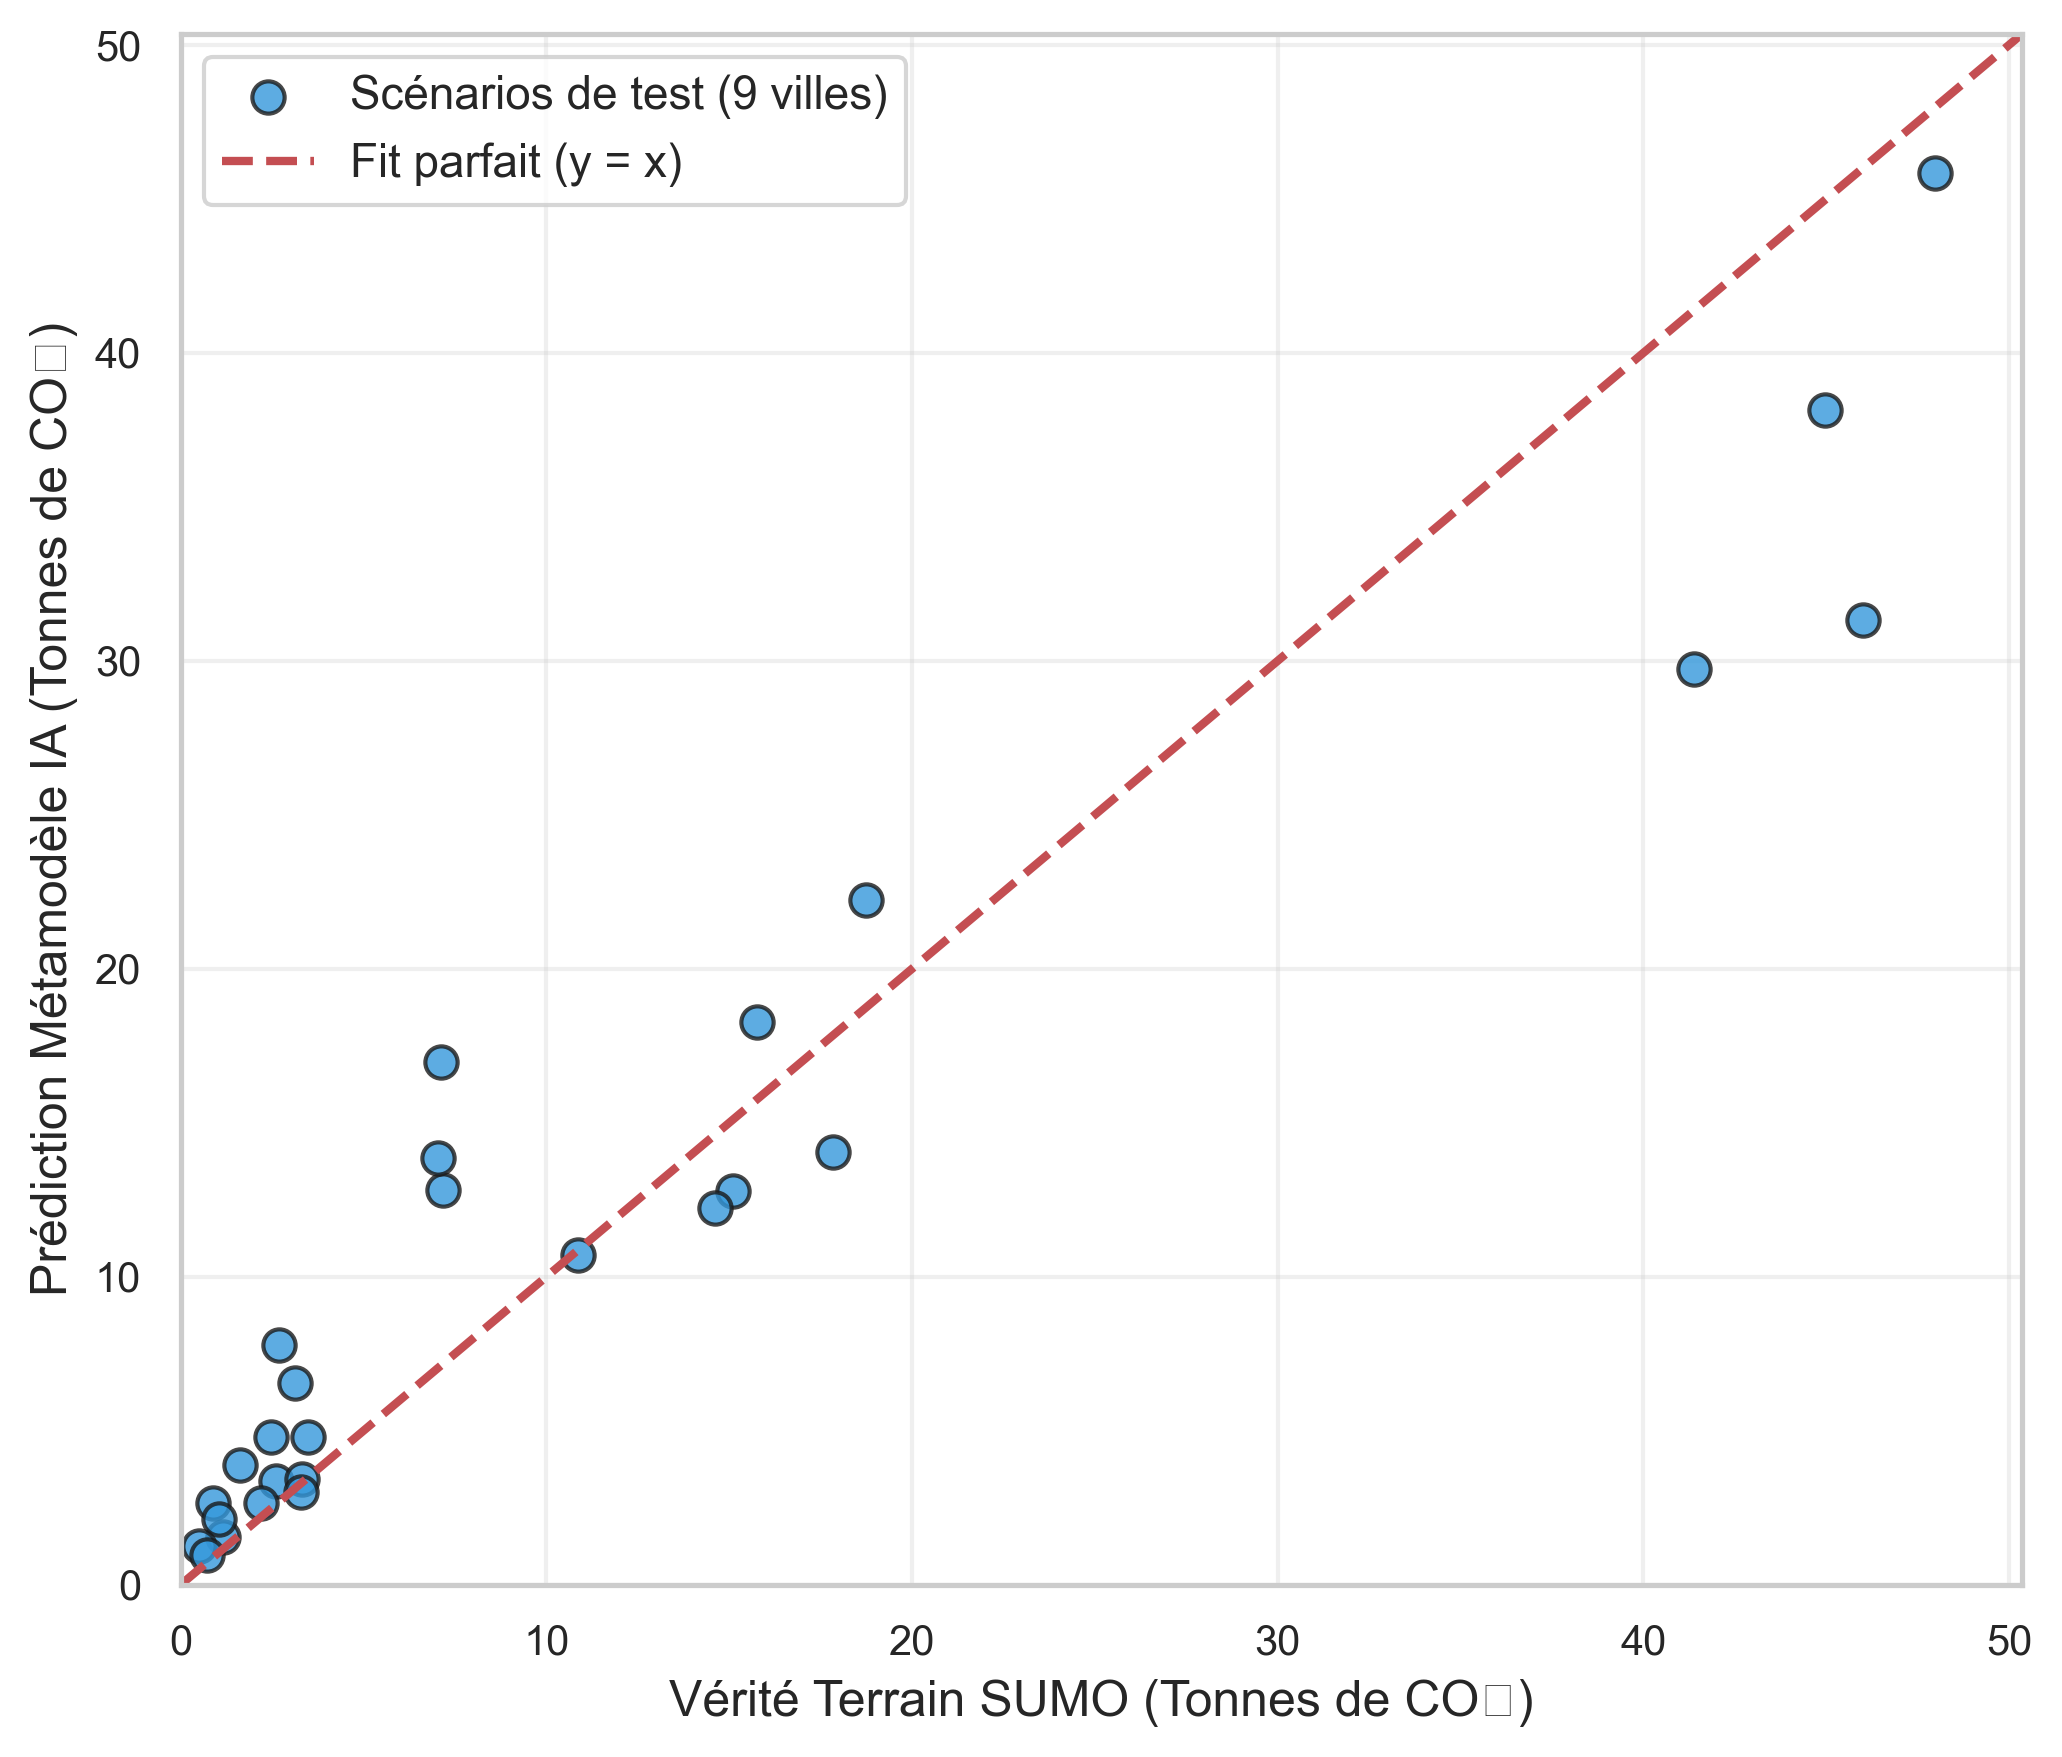
\includegraphics[keepaspectratio,alt={Analyse de corrélation et résidus (Scatter Plot) de comparaison entre le métamodèle IA et la simulation SUMO de référence sur les 27 scénarios de validation croisée}]{images/real_vs_predicted_validation.png}}
\caption{Analyse de corrélation et résidus (Scatter Plot) de comparaison
entre le métamodèle IA et la simulation SUMO de référence sur les 27
scénarios de validation croisée}
\end{figure}

\paragraph{Interface d'aide à la décision : Dashboard
Streamlit}\label{interface-daide-uxe0-la-duxe9cision-dashboard-streamlit}

Pour valoriser opérationnellement notre modèle d'IA prédictif et le
rendre exploitable par des planificateurs urbains non-spécialistes du
code, nous avons développé une interface utilisateur interactive sous
forme de tableau de bord \textbf{Streamlit}. L'application
\texttt{app\_thesis.py} se structure autour d'un design moderne avec une
barre latérale de contrôle globale et \textbf{quatre onglets horizontaux
positionnés en haut de l'écran} pour naviguer entre les différentes
échelles d'analyse.

\subparagraph{A. Organisation structurelle de l'interface
graphique}\label{a.-organisation-structurelle-de-linterface-graphique}

L'application est découpée en quatre sections fonctionnelles :

\begin{enumerate}
\def\labelenumi{\arabic{enumi}.}
\tightlist
\item
  \textbf{Onglet 1 : Tableau de Bord Temporel \& CO₂} : Cet onglet
  permet à l'utilisateur d'estimer instantanément les émissions de CO₂
  pour une ville sélectionnée à une heure précise de la journée. Le
  volume de trafic y est calculé de manière dynamique en fonction de la
  capacité physique du réseau routier et de l'horloge. Il affiche des
  jauges de pollution, le tonnage global et la courbe horaire
  d'évolution.
\item
  \textbf{Onglet 2 : Signatures Spectrales \& Stabilité} : Dévoile
  l'empreinte mathématique intrinsèque de la ville. Il affiche les
  distributions des valeurs propres complexes (magnitude des corridors)
  et des valeurs singulières (redondance des voies), ainsi qu'une jauge
  visualisant le score global de vulnérabilité structurelle aux
  congestions.
\item
  \textbf{Onglet 3 : Comparateur de Graphes (Benchmarking)} : Module
  permettant de comparer directement deux villes (ex : Paris vs Los
  Angeles, ou Tours vs Utrecht) soumises à la même charge de trafic
  relative, pour isoler l'efficacité pure de leur tracé routier.
\item
  \textbf{Onglet 4 : Analyse Spectrale Détaillée par Ville} : Cet onglet
  permet d'explorer de manière exhaustive l'ensemble des descripteurs
  spectraux et physiques calculés pour une ville choisie. Il affiche les
  métriques topologiques, l'asymétrie, les nœuds sources/puits, la
  constante de Kreiss, la non-normalité, les métriques spectrales
  pondérées physiquement, ainsi que le profil SVD complet des 5 valeurs
  singulières et le ratio de concentration \(\sigma_1 / \sigma_4\)
  évaluant la résilience du réseau.
\end{enumerate}

\subparagraph{B. Le système d'horloge dynamique, de capacité nominale et
de
charge}\label{b.-le-systuxe8me-dhorloge-dynamique-de-capacituxe9-nominale-et-de-charge}

Pour éviter la saisie manuelle de données de trafic arbitraires,
l'application couple automatiquement la structure physique du réseau
avec un profil d'activité horaire :

\begin{itemize}
\item
  \textbf{Calcul de la capacité physique nominale (\(C_{ville}\))} : La
  capacité de stockage fluide du réseau est estimée à partir du nombre
  de nœuds du graphe routier (représentant les intersections réelles) :
  \[C_{ville} = |V| \times 5.0\] Le coefficient \(5.0\) représente le
  ratio de véhicules actifs par carrefour requis pour occuper le réseau
  sans créer d'engorgement en régime stabilisé.
\item
  \textbf{Le facteur de charge temporel (\(\alpha_t\))} : La demande de
  trafic fluctue au cours des 24 heures de la journée selon une courbe
  typique de charge en ``M''. La variable \(\alpha_t \in [0.10, 0.95]\)
  exprime la part de capacité routière sollicitée :

  \begin{itemize}
  \tightlist
  \item
    \emph{Heures de pointe (08h00 et 18h00) :} \(\alpha_t = 0.95\)
    (charge maximale).
  \item
    \emph{Heures creuses diurnes (10h00, 14h00) :} \(\alpha_t = 0.45\)
    (trafic modéré).
  \item
    \emph{Heures nocturnes (02h00 - 03h00) :} \(\alpha_t = 0.10\)
    (trafic résiduel).
  \end{itemize}
\item
  \textbf{Calcul du volume de trafic injecté} : Pour toute heure \(t\)
  sélectionnée sur l'horloge interactive, le volume de véhicules à
  évaluer est généré par :
  \[\text{nb\_total\_veh} = C_{ville} \times \alpha_t\] Ce nombre
  alimente instantanément le modèle XGBoost pour prédire le CO₂
  correspondant.
\end{itemize}

\subparagraph{C. Évaluation de la vulnérabilité et de la performance
environnementale}\label{c.-uxe9valuation-de-la-vulnuxe9rabilituxe9-et-de-la-performance-environnementale}

L'interface Streamlit propose deux indicateurs de performance avancés :

\begin{itemize}
\item
  \textbf{L'Indice de Vulnérabilité aux Congestions (\(SV\))} : Il
  quantifie le risque d'amplification transitoire de la congestion
  (phénomène d'onde de choc ou gridlock) en combinant la non-normalité
  relative (\(NN_{rel} = \frac{\|AA^T - A^TA\|_F}{|V|}\)) et la
  constante de Kreiss (\(K\)) du réseau via une double fonction
  d'activation tangente hyperbolique :
  \[SV = 0.4 \times \tanh\left(\frac{NN_{rel}}{2.0}\right) + 0.6 \times \tanh\left(\frac{K}{25.0}\right)\]
  Ce score global normalisé de \(0\,\%\) (sécurité absolue) à
  \(100\,\%\) (sensibilité critique) permet de détecter instantanément
  les villes les plus sensibles aux perturbations locales.
\item
  \textbf{Métrique géométrique neutre (Émissions Spécifiques)} : Le
  comparateur de l'onglet 3 calcule le rapport des émissions globales
  divisé par la flotte injectée :
  \[\text{Émissions Spécifiques} = \frac{\widehat{CO}_2 \text{ (kg)}}{\text{Nombre de véhicules}}\]
  Cela permet de comparer directement l'efficacité d'un maillage (ex :
  grille de Los Angeles vs radial de Paris) en éliminant l'effet de
  taille de la ville.
\item
  \textbf{Taux d'abattement carbone en temps réel} : L'interface calcule
  dynamiquement la réduction d'émissions obtenue grâce aux taux
  d'électrification (EV) choisis sur les barres coulissantes de la
  flotte :
  \[\text{Taux d'abattement (\%)} = \left( 1 - \frac{\widehat{CO}_2(\text{avec EV})}{\widehat{CO}_2(\text{sans EV})} \right) \times 100\]
  Ce taux compare la configuration active avec un scénario fictif 100\%
  thermique de référence pour quantifier le bénéfice écologique immédiat
  de la transition.
\end{itemize}

\begin{figure}
\centering
\pandocbounded{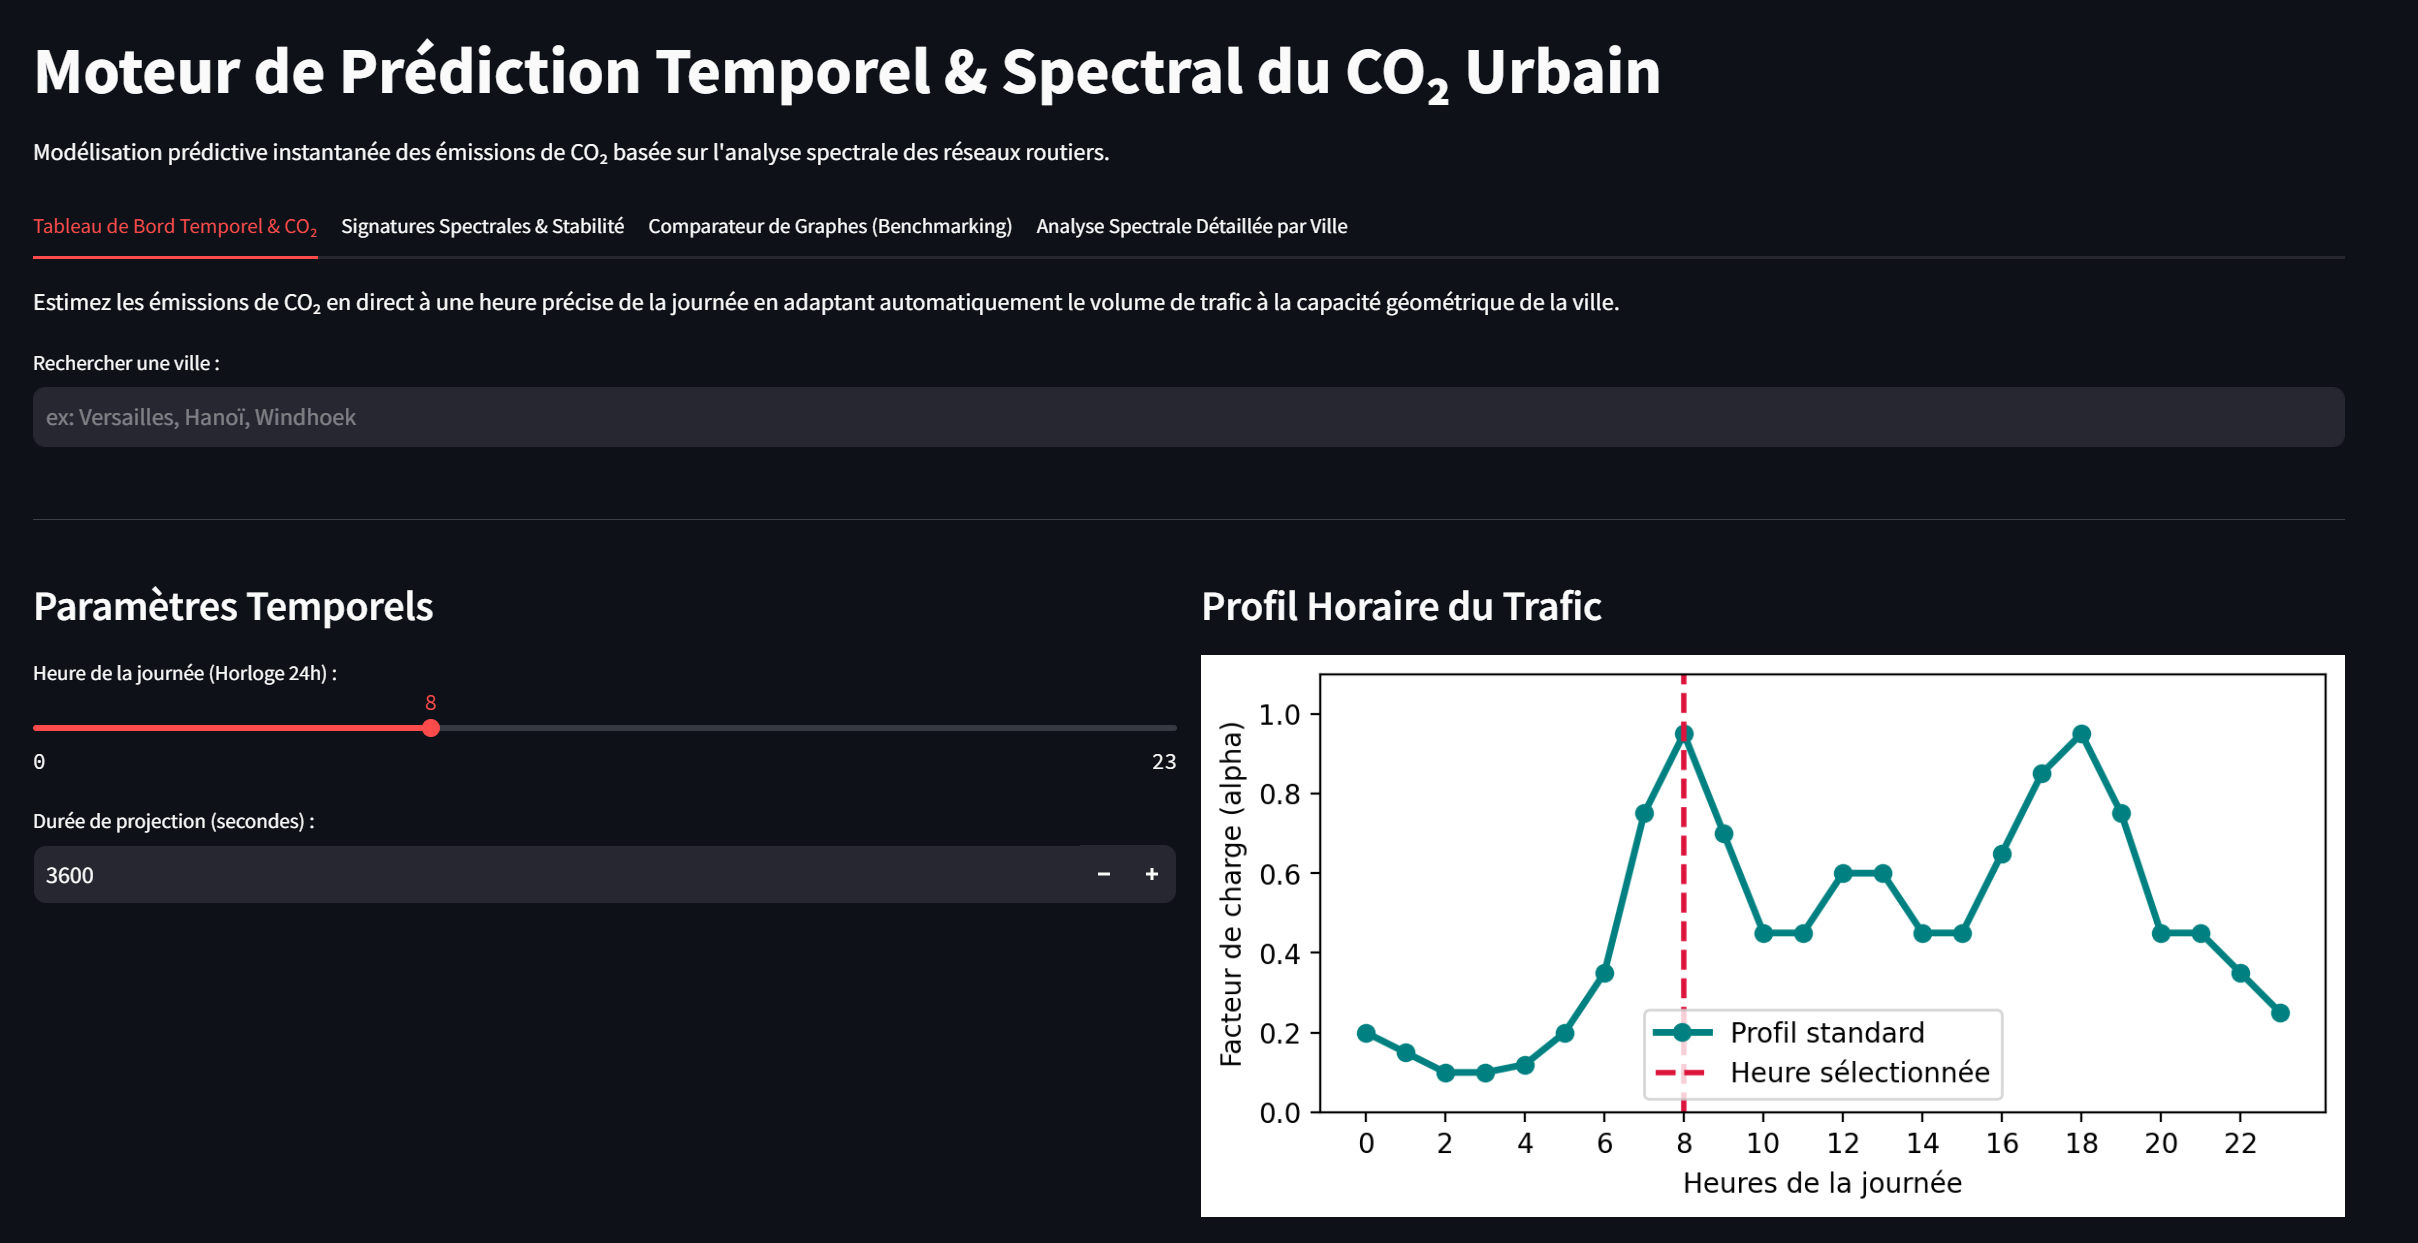
\includegraphics[keepaspectratio,alt={Interface de configuration du dashboard Streamlit - Panneau latéral de configuration de la demande et de l'électromobilité}]{images/streamlit-interface.png}}
\caption{Interface de configuration du dashboard Streamlit - Panneau
latéral de configuration de la demande et de l'électromobilité}
\end{figure}

\textbf{Visualisation des résultats d'émissions de CO₂ instantanés sur
l'interface :} \emph{(L'illustration présentant les courbes et jauges de
prédiction instantanée de CO₂ sur le dashboard sera intégrée dans une
version ultérieure).}

\begin{figure}
\centering
\pandocbounded{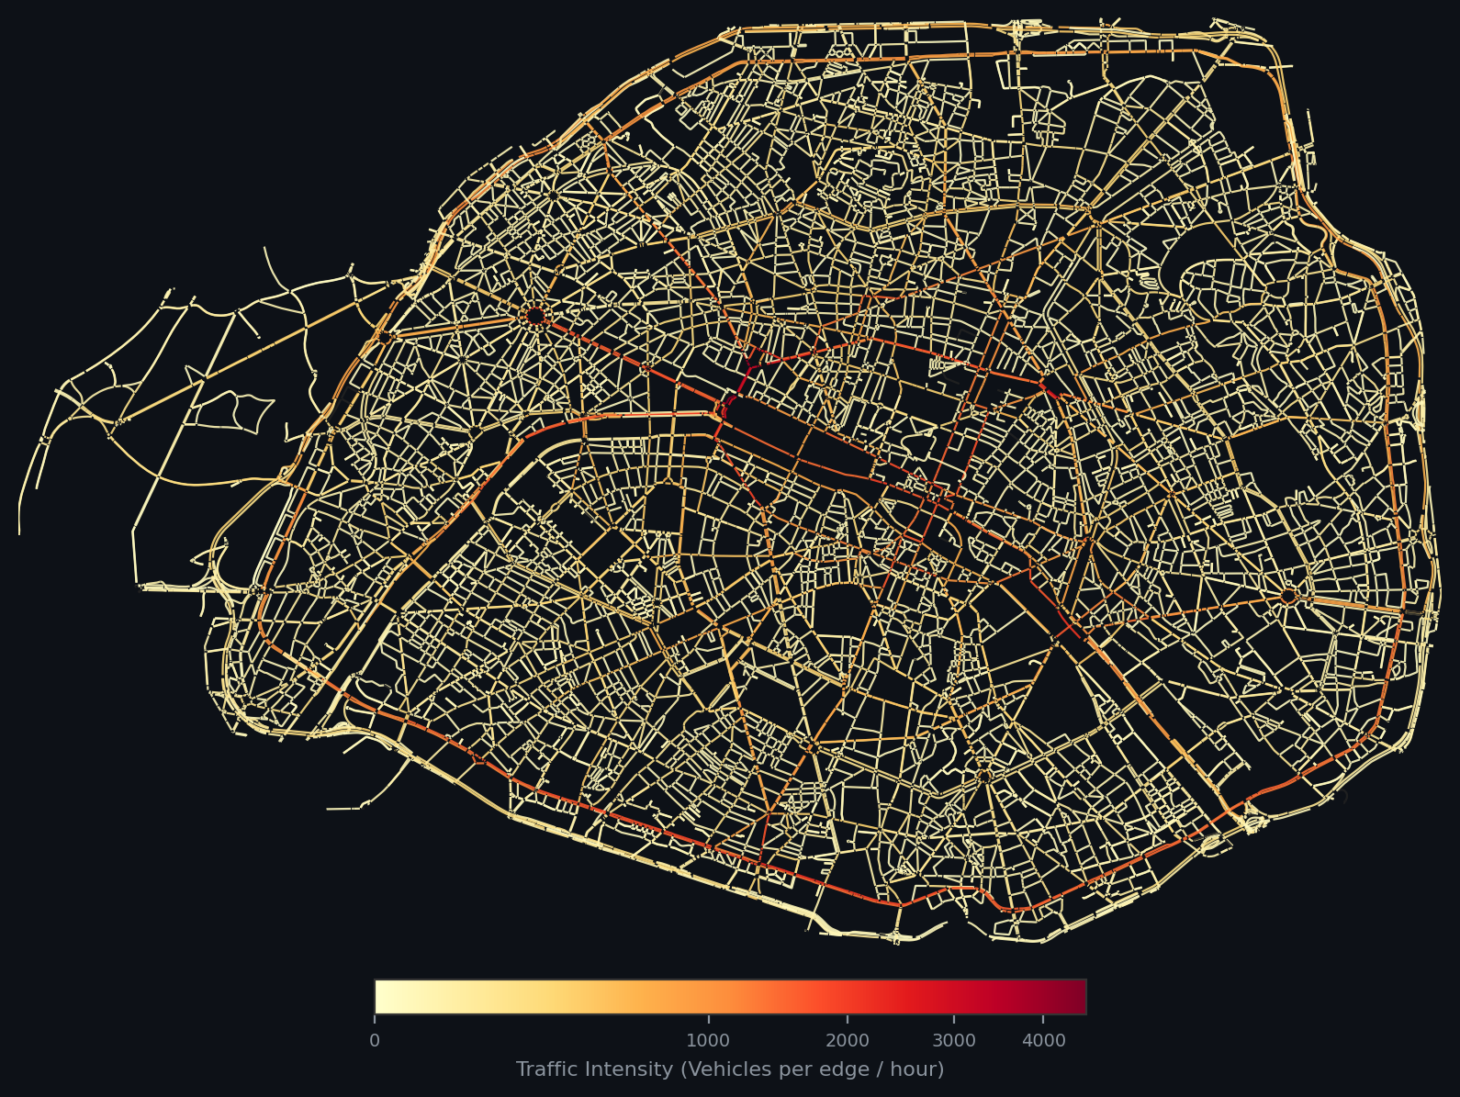
\includegraphics[keepaspectratio,alt={Visualisation SIG de la ville test (Illustration de la cartographie des congestions) - Segments routiers colorés du gris (fluide) au rouge (saturation complète / gridlock)}]{images/paris-heat_map_trafic.png}}
\caption{Visualisation SIG de la ville test (Illustration de la
cartographie des congestions) - Segments routiers colorés du gris
(fluide) au rouge (saturation complète / gridlock)}
\end{figure}

\subsubsection{Section 3 : Perspectives
opérationnelles}\label{section-3-perspectives-opuxe9rationnelles}

La complémentarité des deux approches développées dans ce mémoire ouvre
la voie à un cadre d'optimisation urbaine hybride (IA-SUMO) alliant la
rapidité de l'apprentissage machine et la précision de la simulation
physique. Dans ce schéma opérationnel, le modèle prédictif basé sur l'IA
(XGBoost) est utilisé en amont pour explorer rapidement de larges
espaces de solutions (par exemple, tester des milliers d'implantations
géométriques de voirie ou de localisations de hubs de recharge). L'IA
évalue chaque configuration en une fraction de seconde, éliminant les
scénarios inefficaces et sélectionnant les configurations optimales. Les
scénarios retenus par le modèle prédictif sont ensuite injectés dans le
jumeau numérique microscopique haute-fidélité (SUMO) pour affiner
l'analyse locale (vérification des files d'attente au mètre près,
comportement d'évitement des deux-roues, impact électrique précis).

\paragraph{Modélisation de la sensibilité météorologique et perspectives
d'extension}\label{moduxe9lisation-de-la-sensibilituxe9-muxe9tuxe9orologique-et-perspectives-dextension}

Une perspective d'extension majeure pour accroître la fidélité de notre
métamodèle d'IA réside dans l'intégration systématique des variables
météorologiques (pluie, neige), dont l'impact sur la congestion urbaine
est bien documenté.

\subparagraph{Mécanisme physique de la perturbation
météorologique}\label{muxe9canisme-physique-de-la-perturbation-muxe9tuxe9orologique}

Dans un micro-simulateur comme SUMO, les perturbations climatiques
modifient les paramètres physiques fondamentaux du modèle de poursuite
cinématique de Krauß :

\begin{enumerate}
\def\labelenumi{\arabic{enumi}.}
\tightlist
\item
  \textbf{Vitesse de sécurité (\(v_{safe}\))} : Les précipitations
  diminuent le coefficient d'adhérence des pneumatiques (\(\mu\)). Sous
  la pluie, \(\mu\) passe de \(0,8\) à \(0,5\), et sur la neige il chute
  à \(0,2\). Cela force le modèle de poursuite à diminuer la
  décélération de sécurité \(d\) de \(30\ \%\) (pluie) à \(70\ \%\)
  (neige) dans l'équation de vitesse limite :
  \[v_{safe}(t) = v_L(t) + \frac{g(t) - v_L(t)\tau}{\frac{v(t) + v_L(t)}{2d} + \tau}\]
\item
  \textbf{Imprécision de conduite (\(\sigma\))} : La réduction de la
  visibilité et le stress allongent le temps de réaction effectif des
  conducteurs (\(\tau\)) et augmentent l'imprécision du contrôle
  cinématique (\(\sigma\)), provoquant des fluctuations de vitesse
  stochastiques plus fréquentes.
\end{enumerate}

Dans le formalisme du métamodèle d'IA, ces modifications microscopiques
se traduisent macroscopiquement par une réduction de la vitesse moyenne
globale du réseau (\texttt{avg\_speed\_mps}). Cette baisse de vitesse
allonge la durée de transit des véhicules, déplaçant le point de
fonctionnement sur la courbe de congestion vers des zones d'émissions de
\(CO_2\) exponentielles.

\subparagraph{Coefficients de sensibilité régionaux et
comportementaux}\label{coefficients-de-sensibilituxe9-ruxe9gionaux-et-comportementaux}

L'impact d'une même intempérie sur le trafic varie considérablement
d'une ville à l'autre en fonction du climat local, des habitudes de
conduite des usagers, et de la réactivité des infrastructures
municipales (déneigement, pneus hiver). Le tableau ci-dessous formalise
la grille de coefficients de réduction de vitesse recommandée pour
calibrer les futurs scénarios de simulation et d'inférence de l'IA :

{\def\LTcaptype{none} % do not increment counter
\begin{longtable}[]{@{}
  >{\raggedright\arraybackslash}p{(\linewidth - 6\tabcolsep) * \real{0.2222}}
  >{\raggedright\arraybackslash}p{(\linewidth - 6\tabcolsep) * \real{0.2222}}
  >{\centering\arraybackslash}p{(\linewidth - 6\tabcolsep) * \real{0.2778}}
  >{\centering\arraybackslash}p{(\linewidth - 6\tabcolsep) * \real{0.2778}}@{}}
\toprule\noalign{}
\begin{minipage}[b]{\linewidth}\raggedright
Catégorie de Ville
\end{minipage} & \begin{minipage}[b]{\linewidth}\raggedright
Exemples de Villes
\end{minipage} & \begin{minipage}[b]{\linewidth}\centering
Réduction Pluie
\end{minipage} & \begin{minipage}[b]{\linewidth}\centering
Réduction Neige
\end{minipage} \\
\midrule\noalign{}
\endhead
\bottomrule\noalign{}
\endlastfoot
\textbf{Plaines Européennes} & Paris, Versailles, Londres & \textbf{-10
\% à -15 \%} & \textbf{-20 \% à -35 \%} \\
\textbf{Montagne et Pré-alpes} & Chamonix, Genève & \textbf{-5 \% à -10
\%} & \textbf{-10 \% à -15 \%} \\
\textbf{Climats Chauds \& Mousson} & Hanoï, Casablanca, Le Caire &
\textbf{-20 \% à -30 \%} & \textbf{-50 \% (Gridlock)} \\
\textbf{Régularité Nord-Américaine} & Los Angeles & \textbf{-15 \% à -20
\%} & \textbf{Non applicable} \\
\textbf{Maillage Océanien} & Auckland, Wellington & \textbf{-10 \%} &
\textbf{Non applicable} \\
\end{longtable}
}

\subparagraph{Justifications sociologiques et techniques de la
sensibilité climatique
:}\label{justifications-sociologiques-et-techniques-de-la-sensibilituxe9-climatique}

\begin{itemize}
\tightlist
\item
  \textbf{Plaines Européennes (Paris, Versailles, Londres)} : Usagers
  peu habitués aux conditions hivernales et équipements de déneigement
  municipaux limités. Une faible couche de neige provoque un engorgement
  rapide par panique comportementale.
\item
  \textbf{Montagne et Pré-alpes (Chamonix, Genève)} : Usagers très
  expérimentés, équipements d'hiver obligatoires et services municipaux
  de déneigement réactifs et structurés, minimisant l'impact
  cinématique.
\item
  \textbf{Climats Chauds \& Mousson (Hanoï, Casablanca, Le Caire)} :
  Risques importants d'inondations de chaussées lors des moussons. Les
  épisodes de neige y sont exceptionnels et paralyseraient
  instantanément l'intégralité du réseau.
\item
  \textbf{Régularité Nord-Américaine (Los Angeles)} : Précipitations
  très rares. En cas d'ondée, le manque d'habitude engendre des
  comportements prudents excessifs ou des accrochages en cascade.
\item
  \textbf{Maillage Océanien (Auckland, Wellington)} : Perturbation
  standard principalement liée à la perte d'adhérence et à la baisse de
  visibilité.
\end{itemize}

\subparagraph{Implémentation fonctionnelle dans l'interface
Streamlit}\label{impluxe9mentation-fonctionnelle-dans-linterface-streamlit}

Pour rendre cette sensibilité opérationnelle dans notre dashboard
Streamlit (\texttt{app\_streamlit.py}), nous appliquons directement ces
coefficients de réduction sur la variable d'entrée de la vitesse moyenne
:

\begin{itemize}
\tightlist
\item
  \emph{Régime Clair (Optimal) :} Vitesse moyenne nominale calculée par
  la topologie de la ville (ex. \(25\text{ km/h}\)).
\item
  \emph{Régime Pluvieux :} Réduction automatique de la vitesse de
  \(-10\ \%\) (la vitesse injectée dans le modèle XGBoost passe à
  \(22,5\text{ km/h}\)).
\item
  \emph{Régime Enneigé :} Réduction automatique de la vitesse de
  \(-20\ \%\) (la vitesse appliquée passe à \(20\text{ km/h}\)).
\end{itemize}

Cette modulation de la vitesse d'entrée décale le point d'inférence de
XGBoost vers une zone de charge plus élevée, permettant de prédire
instantanément le surcoût écologique lié à la météo sans devoir relancer
une simulation physique lourde.

Les résultats de ce travail de recherche font d'ailleurs l'objet d'une
valorisation académique à travers la préparation de deux publications
scientifiques de fin d'année. La première publication, co-écrite avec
VinUniversity, s'intitule \emph{``Microscopic Traffic Flow and Emission
Modeling of High-Power Electric Vehicle Charging Infrastructure in
Hyper-Dense Master-Planned Communities: The Case of Sao Bien, Vinhomes
Ocean Park.''} (présentation du protocole YOLOv8, de l'architecture du
jumeau numérique SUMO et de l'évaluation des scénarios de
densification). La deuxième publication s'intitule \emph{``Topological
Graph-Spectral Machine Learning for Real-Time Urban CO2 Emissions
Prediction: Applying Kato's Perturbation Theory and Kreiss Constants to
Non-Normal Urban Networks.''} (formalisation de la méthode de prédiction
spectrale sur graphes non-symétriques, étude de la stabilité via la
constante de Kreiss et performances de XGBoost).

\newpage

\section{CONCLUSION}\label{conclusion}

Ce travail de recherche a permis de jeter les bases d'un double cadre
méthodologique pour la modélisation de la mobilité urbaine décarbonée.
Nos travaux s'articulent ainsi autour d'un double objectif de recherche
complémentaire.

D'une part, nous avons développé des jumeaux numériques microscopiques
de haute-fidélité capables de modéliser l'impact cinématique local de
l'intégration d'infrastructures de recharge pour véhicules électriques.
Ce travail a été appliqué sur le quartier résidentiel à haute densité de
Sao Bien à Hanoï. Il a permis d'intégrer des comportements stochastiques
de charge et de documenter des dynamiques de trafic spécifiques comme
l'inversion modale de vacances (\emph{Holiday Reversal}), le tout
calibré par des données réelles issues de notre protocole de vision par
ordinateur YOLOv8.

D'autre part, nous avons proposé une méthode de rupture basée sur
l'intelligence artificielle topologique spectrale. En exploitant la
structure mathématique de la matrice d'adjacence du réseau urbain (rayon
spectral, constante de Kreiss, perturbations de Kato) et l'algorithme
XGBoost, nous avons démontré qu'il est possible d'estimer instantanément
la pollution d'une ville sans simuler individuellement chaque véhicule,
contournant ainsi les limites computationnelles traditionnelles (RAM,
SWAP) à l'échelle macroscopique.

La boucle d'optimisation hybride (IA-SUMO) constitue la perspective
ultime de ces travaux, permettant d'optimiser l'aménagement urbain à
grande échelle tout en conservant une précision physique sur les points
sensibles du réseau. Enfin, la valorisation académique de ces recherches
à travers la rédaction de deux articles scientifiques de fin d'année
témoigne de la rigueur et de la portée de la méthodologie développée.

\newpage

\section{BIBLIOGRAPHIE SCIENTIFIQUE ET
ACADÉMIQUE}\label{bibliographie-scientifique-et-acaduxe9mique}

\begin{itemize}
\tightlist
\item
  Agarwal, M., Maze, T. H., \& Souleyrette, R. (2005). \emph{Impacts of
  Weather on Urban Freeway Traffic Flow Characteristics and Facility
  Capacity}. Center for Transportation Research and Education, Iowa
  State University.
\item
  Boeing, G. (2017). \emph{OSMnx: New methods for acquiring,
  constructing, analyzing, and visualizing complex street networks}.
  Computers, Environment and Urban Systems, 65, 126-139.
\item
  Braess, D. (1968). \emph{Über ein Paradoxon aus der Verkehrsplanung}.
  Unternehmensforschung, 12, 258-268.
\item
  Easley, D., \& Kleinberg, J. (2010). \emph{Networks, Crowds, and
  Markets: Reasoning about a Highly Connected World}. Cambridge
  University Press.
\item
  Forrester, J. W. (1969). \emph{Urban Dynamics}. Productivity Press.
\item
  Kato, T. (1995). \emph{Perturbation Theory for Linear Operators} (Vol.
  132). Springer Science \& Business Media.
\item
  Krajzewicz, D., Erdmann, J., Behrisch, M., \& Bieker, L. (2012).
  \emph{Recent development and applications of SUMO - Simulation of
  Urban MObility}. International Journal on Advances in Systems and
  Measurements, 5(3\&4), 128-138.
\item
  Kratzsch, V. et al.~(2020). \emph{HBEFA Version 4.1 -- Handbook
  Emission Factors for Road Transport}. INFRAS.
\item
  Kreiss, H. O. (1962). \emph{Über die Stabilitätsdefinition für
  Differenzengleichungen, die partielle Differentialgleichungen
  approximieren}. BIT Numerical Mathematics, 2(3), 153-181.
\item
  Mitchell, M. (2009). \emph{Complexity: A Guided Tour}. Oxford
  University Press.
\item
  Thocle (2025). \emph{Realistic Urban Traffic Generator using
  Decentralized Federated Learning for the SUMO simulator}.
  arXiv:2506.07980.
\item
  Trefethen, L. N., \& Embree, M. (2005). \emph{Spectra and
  Pseudospectra: The Behavior of Nonnormal Matrices and Operators}.
  Princeton University Press.
\end{itemize}

\newpage

\section{RÉFÉRENCES WEB ET INSTITUTIONNELLES
(WEBOGRAPHIE)}\label{ruxe9fuxe9rences-web-et-institutionnelles-webographie}

\begin{itemize}
\tightlist
\item
  Aimsun (2024). \emph{Aimsun Next User Manual}. Aimsun SLU.
  \url{https://www.aimsun.com/}
\item
  Apur (2025). \emph{Évolution des mobilités et du parc automobile dans
  la Métropole du Grand Paris au 1er Janvier 2025}. Atelier Parisien
  d'Urbanisme.
\item
  Avere-France (2025). \emph{Baromètre national des infrastructures de
  recharge de véhicules électriques}.
  \url{https://www.avere-france.org/}
\item
  City of Paris (2024). \emph{Rapport d'activité sur les déplacements et
  la circulation à Paris en 2023}. Mairie de Paris.
\item
  European Environment Agency (EEA) (2024). \emph{Transport and
  Mobility: Transitioning to Sustainable Systems}. EEA Report.
  \url{https://www.eea.europa.eu/}
\item
  French Government (2026). \emph{Bonus écologique et primes pour
  l'acquisition d'un véhicule électrique}. Service-Public.fr.
  \url{https://www.service-public.fr/}
\item
  Green SM (2025). \emph{GSM: Green and Smart Mobility electric fleet
  expansion}. GSM Joint Stock Company. \url{https://www.green-sm.com/}
\item
  International Energy Agency (IEA) (2025). \emph{Road Transport --
  Breakthrough Agenda Report 2025}. IEA. \url{https://www.iea.org/}
\item
  MATsim (2024). \emph{Multi-Agent Transport Simulation (MATSim)
  Documentation}. MATsim Community. \url{https://www.matsim.org/}
\item
  OECD (2024). \emph{Urban Mobility and Decarbonisation}. Organisation
  for Economic Co-operation and Development. \url{https://www.oecd.org/}
\item
  PTV Group (2024). \emph{PTV Vissim User Manual: Microscopic Traffic
  Flow Simulation}. \url{https://www.ptvgroup.com/}
\item
  Streamlit Inc.~(2020). \emph{Streamlit: The fastest way to build and
  share data applications for machine learning}.
  \url{https://streamlit.io/}
\item
  SUMO (2024). \emph{SUMO User Documentation}. German Aerospace Center
  (DLR). \url{https://sumo.dlr.de/}
\item
  Texas A\&M Transportation Institute (2021). \emph{Urban Mobility
  Report}. Texas A\&M University. \url{https://mobility.tamu.edu/}
\item
  United Nations, Department of Economic and Social Affairs (2018).
  \emph{World Urbanization Prospects: The 2018 Revision}. United
  Nations. \url{https://www.un.org/}
\item
  United Nations, Department of Economic and Social Affairs (2018).
  \emph{Sustainable Urbanization is Key to Successful Development}.
  United Nations. \url{https://www.un.org/}
\item
  VinBus (2021). \emph{VinBus officially operates the first smart
  electric bus in Vietnam}. VinBus Ecology Transport Services.
  \url{https://vinbus.vn/}
\item
  Vinhomes (2024). \emph{Vinhomes Ocean Park: Urban Development and
  Master-Planned Communities}. Vinhomes Joint Stock Company.
  \url{https://oceanpark.vinhomes.vn/}
\item
  World Bank (2024). \emph{Urban Development Overview}. World Bank
  Group. \url{https://www.worldbank.org/}
\end{itemize}

\newpage

\section{ANNEXES : TABLEAUX COMPLÉMENTAIRES DES RUNS DE SIMULATION
MULTI-VILLES}\label{annexes-tableaux-compluxe9mentaires-des-runs-de-simulation-multi-villes}

\subsubsection{Tableau 7 : Extrait des indicateurs macroscopiques des
simulations de
référence}\label{tableau-7-extrait-des-indicateurs-macroscopiques-des-simulations-de-ruxe9fuxe9rence}

{\def\LTcaptype{none} % do not increment counter
\begin{longtable}[]{@{}
  >{\raggedright\arraybackslash}p{(\linewidth - 14\tabcolsep) * \real{0.1053}}
  >{\raggedright\arraybackslash}p{(\linewidth - 14\tabcolsep) * \real{0.1053}}
  >{\centering\arraybackslash}p{(\linewidth - 14\tabcolsep) * \real{0.1316}}
  >{\centering\arraybackslash}p{(\linewidth - 14\tabcolsep) * \real{0.1316}}
  >{\centering\arraybackslash}p{(\linewidth - 14\tabcolsep) * \real{0.1316}}
  >{\centering\arraybackslash}p{(\linewidth - 14\tabcolsep) * \real{0.1316}}
  >{\centering\arraybackslash}p{(\linewidth - 14\tabcolsep) * \real{0.1316}}
  >{\centering\arraybackslash}p{(\linewidth - 14\tabcolsep) * \real{0.1316}}@{}}
\toprule\noalign{}
\begin{minipage}[b]{\linewidth}\raggedright
Date \& Time
\end{minipage} & \begin{minipage}[b]{\linewidth}\raggedright
City
\end{minipage} & \begin{minipage}[b]{\linewidth}\centering
Vehicles
\end{minipage} & \begin{minipage}[b]{\linewidth}\centering
Avg Speed
\end{minipage} & \begin{minipage}[b]{\linewidth}\centering
CO₂ Emitted
\end{minipage} & \begin{minipage}[b]{\linewidth}\centering
Weather
\end{minipage} & \begin{minipage}[b]{\linewidth}\centering
EV Adoption
\end{minipage} & \begin{minipage}[b]{\linewidth}\centering
Execution Time
\end{minipage} \\
\midrule\noalign{}
\endhead
\bottomrule\noalign{}
\endlastfoot
2026-06-08 11:37:40 & \textbf{Sydney} & 47 239 & 2.76 km/h & 174.23 Tons
& Clear (Optimal) & 15\% & 2602.90 s \\
2026-06-08 10:15:27 & \textbf{Rio de Janeiro} & 64 172 & 2.72 km/h &
265.52 Tons & Clear (Optimal) & 15\% & 3787.60 s \\
2026-06-08 09:58:55 & \textbf{Monaco} & 6 080 & 5.86 km/h & 21.46 Tons &
Clear (Optimal) & 8\% & 185.89 s \\
2026-06-06 10:55:18 & \textbf{Casablanca} & 49 785 & 15.62 km/h & 172.64
Tons & Clear (Optimal) & 10\% & 17605.75 s \\
2026-06-06 09:30:40 & \textbf{London} & 68 239 & 1.52 km/h & 241.86 Tons
& Clear (Optimal) & 15\% & 4545.16 s \\
2026-05-22 11:31:03 & \textbf{Sydney} & 55 453 & 2.21 km/h & 215.45 Tons
& Clear (Optimal) & 15\% & 3752.45 s \\
2026-05-22 10:33:58 & \textbf{Chamonix} & 2 000 & 46.50 km/h & 2.32 Tons
& Clear (Optimal) & 8\% & 13.07 s \\
2026-05-21 11:54:12 & \textbf{Versailles} & 1 000 & 31.46 km/h & 0.76
Tons & Clear (Optimal) & 10\% & 18.96 s \\
2026-05-13 20:22:36 & \textbf{Versailles} & 20 450 & 2.31 km/h & 82.06
Tons & Clear (Optimal) & 10\% & 521.54 s \\
2026-05-12 15:36:46 & \textbf{Madrid} & 98 560 & 16.19 km/h & 352.83
Tons & Clear (Optimal) & 10\% & 12276.98 s \\
2026-05-12 11:03:53 & \textbf{Paris} & 128 644 & 3.08 km/h & 508.20 Tons
& Clear (Optimal) & 10\% & 5971.15 s \\
2026-04-13 06:07:41 & \textbf{Paris} & 92 173 & 4.75 km/h & 338.01 Tons
& Clear (Optimal) & 10\% & 4126.56 s \\
2026-04-12 12:14:49 & \textbf{Paris} & 90 909 & 4.06 km/h & 341.46 Tons
& Clear (Optimal) & 10\% & 4340.81 s \\
2026-04-12 08:06:36 & \textbf{Paris} & 48 554 & 8.74 km/h & 152.21 Tons
& Clear (Optimal) & N/A & 2036.43 s \\
2026-04-11 16:47:14 & \textbf{Paris} & 48 641 & 7.93 km/h & 151.69 Tons
& Clear (Optimal) & N/A & 2051.00 s \\
2026-04-11 16:11:53 & \textbf{Versailles} & 12 750 & 4.26 km/h & 49.45
Tons & Clear (Optimal) & N/A & 219.36 s \\
2026-04-11 13:25:05 & \textbf{Paris} & 48 669 & 9.09 km/h & 166.46 Tons
& Clear (Optimal) & N/A & 2039.20 s \\
\end{longtable}
}

\subsubsection{\texorpdfstring{Tableau 8 : Répartition des tonnages de
\(CO_2\) émis par classe de véhicule de la
flotte}{Tableau 8 : Répartition des tonnages de CO\_2 émis par classe de véhicule de la flotte}}\label{tableau-8-ruxe9partition-des-tonnages-de-co_2-uxe9mis-par-classe-de-vuxe9hicule-de-la-flotte}

{\def\LTcaptype{none} % do not increment counter
\begin{longtable}[]{@{}
  >{\raggedright\arraybackslash}p{(\linewidth - 12\tabcolsep) * \real{0.1212}}
  >{\raggedright\arraybackslash}p{(\linewidth - 12\tabcolsep) * \real{0.1212}}
  >{\centering\arraybackslash}p{(\linewidth - 12\tabcolsep) * \real{0.1515}}
  >{\centering\arraybackslash}p{(\linewidth - 12\tabcolsep) * \real{0.1515}}
  >{\centering\arraybackslash}p{(\linewidth - 12\tabcolsep) * \real{0.1515}}
  >{\centering\arraybackslash}p{(\linewidth - 12\tabcolsep) * \real{0.1515}}
  >{\centering\arraybackslash}p{(\linewidth - 12\tabcolsep) * \real{0.1515}}@{}}
\toprule\noalign{}
\begin{minipage}[b]{\linewidth}\raggedright
Date \& Time
\end{minipage} & \begin{minipage}[b]{\linewidth}\raggedright
City
\end{minipage} & \begin{minipage}[b]{\linewidth}\centering
Total CO₂
\end{minipage} & \begin{minipage}[b]{\linewidth}\centering
Cars CO₂
\end{minipage} & \begin{minipage}[b]{\linewidth}\centering
Motorcycles CO₂
\end{minipage} & \begin{minipage}[b]{\linewidth}\centering
Buses CO₂
\end{minipage} & \begin{minipage}[b]{\linewidth}\centering
Trucks CO₂
\end{minipage} \\
\midrule\noalign{}
\endhead
\bottomrule\noalign{}
\endlastfoot
2026-06-08 11:37:40 & \textbf{Sydney} & \textbf{174.23 T} & 88.43 T &
37.37 T & 23.26 T & 25.18 T \\
2026-06-08 10:15:27 & \textbf{Rio de Janeiro} & \textbf{265.52 T} &
134.77 T & 56.41 T & 36.30 T & 38.04 T \\
2026-06-08 09:58:55 & \textbf{Monaco} & \textbf{21.46 T} & 17.24 T &
2.26 T & 0.95 T & 1.01 T \\
2026-06-06 10:55:18 & \textbf{Casablanca} & \textbf{172.64 T} & 104.59 T
& 26.36 T & 24.60 T & 17.09 T \\
2026-06-06 09:30:40 & \textbf{London} & \textbf{241.86 T} & 123.13 T &
53.54 T & 31.05 T & 34.14 T \\
2026-05-22 11:31:03 & \textbf{Sydney} & \textbf{215.45 T} & 109.64 T &
46.80 T & 28.13 T & 30.89 T \\
2026-05-22 10:33:58 & \textbf{Chamonix} & \textbf{2.32 T} & 1.88 T &
0.23 T & 0.11 T & 0.10 T \\
2026-05-21 11:54:12 & \textbf{Versailles} & \textbf{0.76 T} & 0.54 T &
0.12 T & 0.08 T & 0.03 T \\
2026-05-13 20:22:36 & \textbf{Versailles} & \textbf{82.06 T} & 57.07 T &
14.03 T & 7.12 T & 3.83 T \\
2026-05-12 15:36:46 & \textbf{Madrid} & \textbf{352.83 T} & 178.47 T &
79.62 T & 55.68 T & 39.05 T \\
2026-05-12 11:03:53 & \textbf{Paris} & \textbf{508.20 T} & 374.95 T &
105.01 T & 9.15 T & 19.10 T \\
2026-04-13 06:07:41 & \textbf{Paris} & \textbf{338.01 T} & 270.84 T &
47.96 T & 6.28 T & 12.93 T \\
2026-04-12 12:14:49 & \textbf{Paris} & \textbf{341.46 T} & 155.06 T &
88.45 T & 63.24 T & 34.71 T \\
2026-04-12 08:06:36 & \textbf{Paris} & \textbf{152.21 T} & 69.28 T &
38.10 T & 29.29 T & 15.53 T \\
2026-04-11 16:47:14 & \textbf{Paris} & \textbf{151.69 T} & 68.97 T &
38.21 T & 29.13 T & 15.38 T \\
2026-04-11 16:11:53 & \textbf{Versailles} & \textbf{49.45 T} & 0.00 T &
0.00 T & 0.00 T & 0.00 T \\
2026-04-11 13:25:05 & \textbf{Paris} & \textbf{166.46 T} & 0.00 T & 0.00
T & 0.00 T & 0.00 T \\
\end{longtable}
}

\subsubsection{Tableau 9 : Profil de performance informatique détaillé
(secondes
CPU)}\label{tableau-9-profil-de-performance-informatique-duxe9tailluxe9-secondes-cpu}

{\def\LTcaptype{none} % do not increment counter
\begin{longtable}[]{@{}
  >{\raggedright\arraybackslash}p{(\linewidth - 10\tabcolsep) * \real{0.1429}}
  >{\raggedright\arraybackslash}p{(\linewidth - 10\tabcolsep) * \real{0.1429}}
  >{\centering\arraybackslash}p{(\linewidth - 10\tabcolsep) * \real{0.1786}}
  >{\centering\arraybackslash}p{(\linewidth - 10\tabcolsep) * \real{0.1786}}
  >{\centering\arraybackslash}p{(\linewidth - 10\tabcolsep) * \real{0.1786}}
  >{\centering\arraybackslash}p{(\linewidth - 10\tabcolsep) * \real{0.1786}}@{}}
\toprule\noalign{}
\begin{minipage}[b]{\linewidth}\raggedright
Date \& Time
\end{minipage} & \begin{minipage}[b]{\linewidth}\raggedright
City
\end{minipage} & \begin{minipage}[b]{\linewidth}\centering
Dijkstra Routing
\end{minipage} & \begin{minipage}[b]{\linewidth}\centering
SUMO Physics Engine
\end{minipage} & \begin{minipage}[b]{\linewidth}\centering
XML Parsing
\end{minipage} & \begin{minipage}[b]{\linewidth}\centering
Total Duration
\end{minipage} \\
\midrule\noalign{}
\endhead
\bottomrule\noalign{}
\endlastfoot
2026-06-08 11:37:40 & \textbf{Sydney} & 666.64 s & 1934.63 s & 1.58 s &
\textbf{2602.90 s} \\
2026-06-08 10:15:27 & \textbf{Rio de Janeiro} & 555.46 s & 3229.83 s &
2.30 s & \textbf{3787.60 s} \\
2026-06-08 09:58:55 & \textbf{Monaco} & 7.69 s & 178.03 s & 0.16 s &
\textbf{185.89 s} \\
2026-06-06 10:55:18 & \textbf{Casablanca} & 13577.62 s & 4026.18 s &
1.89 s & \textbf{17605.75 s} \\
2026-06-06 09:30:40 & \textbf{London} & 1886.52 s & 2655.74 s & 2.90 s &
\textbf{4545.16 s} \\
2026-05-22 11:31:03 & \textbf{Sydney} & 997.87 s & 2752.49 s & 2.08 s &
\textbf{3752.45 s} \\
2026-05-22 10:33:58 & \textbf{Chamonix} & 4.27 s & 8.75 s & 0.04 s &
\textbf{13.07 s} \\
2026-05-21 11:54:12 & \textbf{Versailles} & 6.07 s & 12.84 s & 0.03 s &
\textbf{18.96 s} \\
2026-05-13 20:22:36 & \textbf{Versailles} & 48.35 s & 472.63 s & 0.55 s
& \textbf{521.54 s} \\
2026-05-12 15:36:46 & \textbf{Madrid} & 9716.06 s & 2558.17 s & 2.72 s &
\textbf{12276.98 s} \\
2026-05-12 11:03:53 & \textbf{Paris} & 3371.01 s & 2596.00 s & 4.13 s &
\textbf{5971.15 s} \\
2026-04-13 06:07:41 & \textbf{Paris} & 2353.06 s & 1770.98 s & 2.50 s &
\textbf{4126.56 s} \\
2026-04-12 12:14:49 & \textbf{Paris} & 2421.37 s & 1916.28 s & 3.16 s &
\textbf{4340.81 s} \\
2026-04-12 08:06:36 & \textbf{Paris} & 1167.02 s & 868.03 s & 1.37 s &
\textbf{2036.43 s} \\
2026-04-11 16:47:14 & \textbf{Paris} & 1134.40 s & 915.39 s & 1.20 s &
\textbf{2051.00 s} \\
2026-04-11 16:11:53 & \textbf{Versailles} & 17.36 s & 201.73 s & 0.26 s
& \textbf{219.36 s} \\
2026-04-11 13:25:05 & \textbf{Paris} & 1145.37 s & 892.65 s & 1.17 s &
\textbf{2039.20 s} \\
\end{longtable}
}

\end{document}
